% Options for packages loaded elsewhere
\PassOptionsToPackage{unicode}{hyperref}
\PassOptionsToPackage{hyphens}{url}
\PassOptionsToPackage{dvipsnames,svgnames*,x11names*}{xcolor}
%
\documentclass[
]{krantz}
\usepackage{pdfpages}
\usepackage{lmodern}
\usepackage{amssymb,amsmath}
\usepackage{ifxetex,ifluatex}
\ifnum 0\ifxetex 1\fi\ifluatex 1\fi=0 % if pdftex
  \usepackage[T1]{fontenc}
  \usepackage[utf8]{inputenc}
  \usepackage{textcomp} % provide euro and other symbols
\else % if luatex or xetex
  \usepackage{unicode-math}
  \defaultfontfeatures{Scale=MatchLowercase}
  \defaultfontfeatures[\rmfamily]{Ligatures=TeX,Scale=1}
  \setmonofont[Scale=0.7]{Source Code Pro}
\fi
% Use upquote if available, for straight quotes in verbatim environments
\IfFileExists{upquote.sty}{\usepackage{upquote}}{}
\IfFileExists{microtype.sty}{% use microtype if available
  \usepackage[]{microtype}
  \UseMicrotypeSet[protrusion]{basicmath} % disable protrusion for tt fonts
}{}
\makeatletter
\@ifundefined{KOMAClassName}{% if non-KOMA class
  \IfFileExists{parskip.sty}{%
    \usepackage{parskip}
  }{% else
    \setlength{\parindent}{0pt}
    \setlength{\parskip}{6pt plus 2pt minus 1pt}}
}{% if KOMA class
  \KOMAoptions{parskip=half}}
\makeatother
\usepackage{xcolor}
\IfFileExists{xurl.sty}{\usepackage{xurl}}{} % add URL line breaks if available
\IfFileExists{bookmark.sty}{\usepackage{bookmark}}{\usepackage{hyperref}}
\hypersetup{
  pdftitle={Nova Scotia Atlee Perinatal Database},
  pdfauthor={Reproductive Care Program of Nova Scotia},
  colorlinks=true,
  linkcolor=Maroon,
  filecolor=Maroon,
  citecolor=Blue,
  urlcolor=Blue,
  pdfcreator={LaTeX via pandoc}}
\urlstyle{same} % disable monospaced font for URLs
\usepackage{longtable,booktabs}
% Correct order of tables after \paragraph or \subparagraph
\usepackage{etoolbox}
\makeatletter
\patchcmd\longtable{\par}{\if@noskipsec\mbox{}\fi\par}{}{}
\makeatother
% Allow footnotes in longtable head/foot
\IfFileExists{footnotehyper.sty}{\usepackage{footnotehyper}}{\usepackage{footnote}}
\makesavenoteenv{longtable}
\usepackage{graphicx}
\makeatletter
\def\maxwidth{\ifdim\Gin@nat@width>\linewidth\linewidth\else\Gin@nat@width\fi}
\def\maxheight{\ifdim\Gin@nat@height>\textheight\textheight\else\Gin@nat@height\fi}
\makeatother
% Scale images if necessary, so that they will not overflow the page
% margins by default, and it is still possible to overwrite the defaults
% using explicit options in \includegraphics[width, height, ...]{}
\setkeys{Gin}{width=\maxwidth,height=\maxheight,keepaspectratio}
% Set default figure placement to htbp
\makeatletter
\def\fps@figure{htbp}
\makeatother
\setlength{\emergencystretch}{3em} % prevent overfull lines
\providecommand{\tightlist}{%
  \setlength{\itemsep}{0pt}\setlength{\parskip}{0pt}}
\setcounter{secnumdepth}{5}
\usepackage{pdfpages}
\frontmatter
\usepackage{booktabs}
\usepackage{longtable}
\usepackage{array}
\usepackage{multirow}
\usepackage{wrapfig}
\usepackage{float}
\usepackage{colortbl}
\usepackage{pdflscape}
\usepackage{tabu}
\usepackage{threeparttable}
\usepackage{threeparttablex}
\usepackage[normalem]{ulem}
\usepackage{makecell}
\usepackage{xcolor}

\title{Nova Scotia Atlee Perinatal Database}
\usepackage{etoolbox}
\makeatletter
\providecommand{\subtitle}[1]{% add subtitle to \maketitle
  \apptocmd{\@title}{\par {\large #1 \par}}{}{}
}
\makeatother
\subtitle{Report of Indicators: 2011-2020}
\author{Reproductive Care Program of Nova Scotia}
\date{2023-08-29}

\begin{document}
\pagestyle{empty}
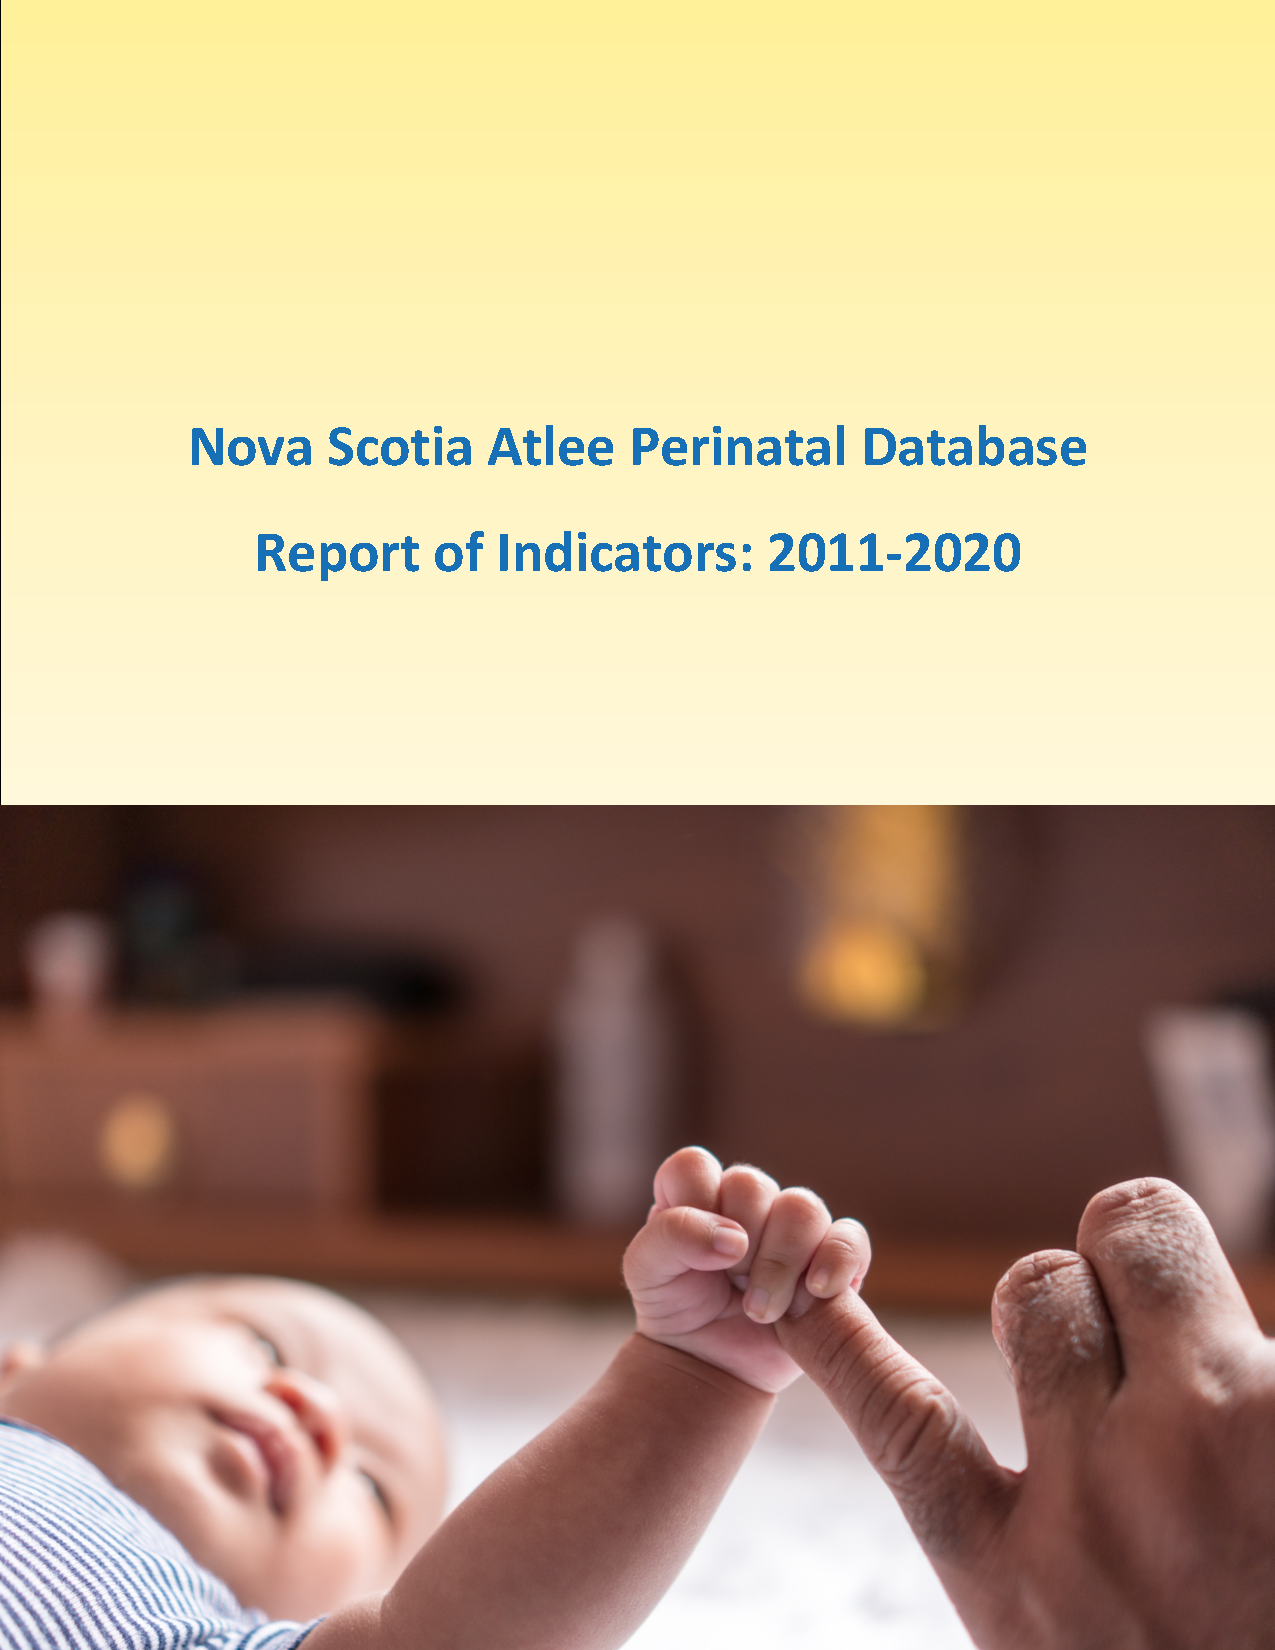
\includepdf{images/Cover2011-2020.pdf}
\setcounter{page}{1}
\maketitle
\thispagestyle{empty}
\newpage


{
\hypersetup{linkcolor=}
\setcounter{tocdepth}{3}
\tableofcontents
\newpage
}


\hypertarget{dedication}{%
\chapter*{Dedication}\label{dedication}}


We would like to dedicate this year's report to Becky Attenborough. The Nova Scotia Atlee Perinatal Database (NSAPD), upon which this report of perinatal indicator is based, has been managed since its inception in 1980 by the Reproductive Care Program (RCP) of Nova Scotia. Rebecca (Becky) Attenborough has managed RCP for the past 30 years. We say good-bye to Becky in this role with sadness but, on the other hand, with the greatest wishes for a well-earned and happy retirement.

Becky's tireless dedication to the role has contributed to the success of the NSAPD in immeasurable ways. On the technical side, Becky shepherded the transition from legacy software into a modern relational database. To do so required the utmost administrative skill to ensure facilities were willing and able to contribute uninterrupted data despite reorganizations and resource reallocation. At the heart of her success is Becky's decade of experience with vulnerable newborns from across the province as a neonatal intensive care nurse and later as head nurse. The knowledge and compassion that she accumulated was incorporated into the development of the NSAPD with substantial influence on the amount and relevance of clinical information captured and incorporating standardized reporting. Most importantly, Becky has been the single biggest user of the NSAPD to guide the planning and management of perinatal care provision, facilitate research, and support the invaluable quality review work that she
and her team of perinatal nurse consultants have undertaken across the province alongside RCP's medical advisors. Her encyclopedic knowledge of the perinatal care provided throughout the province, keen eye for detail, relentless work ethic, and indefatigable good humour have been essential in the survival and success of the NSAPD.

We sincerely thank Becky for her substantial contributions. They have and will continue to benefit all Nova Scotians by ensuring optimal health and well-being of mothers and their newborns.

\begin{center}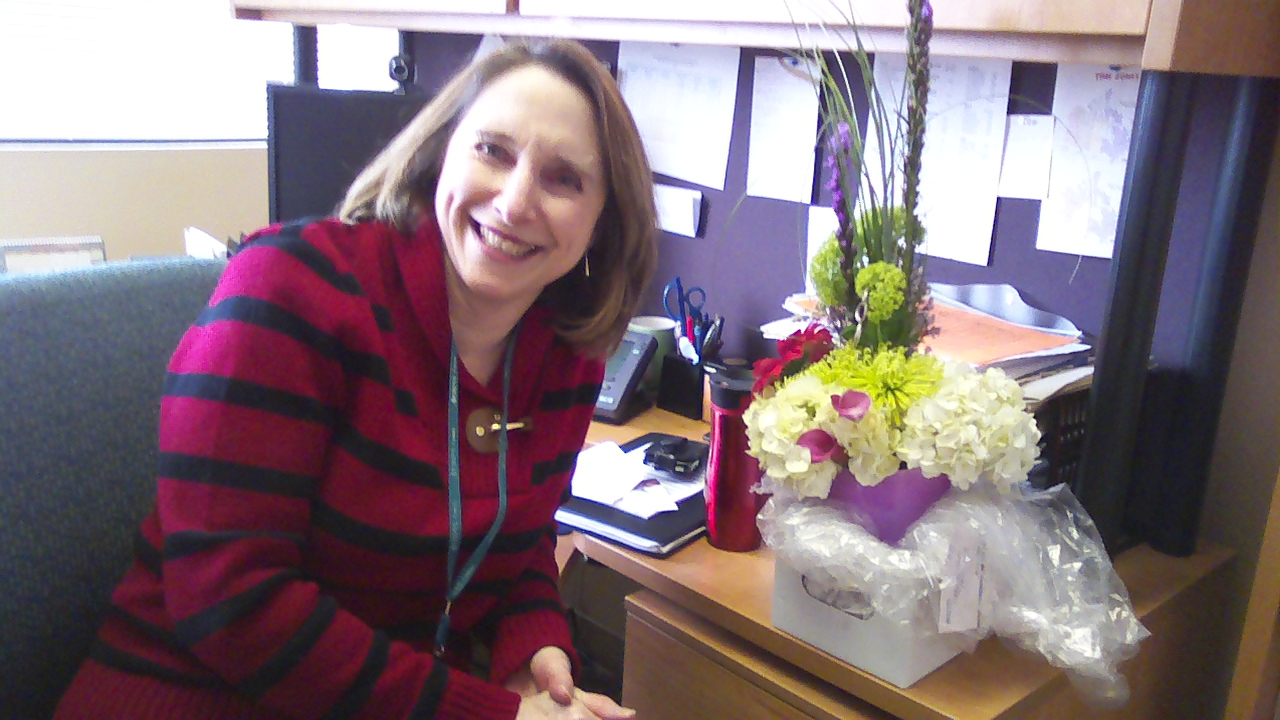
\includegraphics[width=0.4\linewidth]{images/Becky20} \end{center}

\hypertarget{acknowledgements}{%
\chapter*{Acknowledgements}\label{acknowledgements}}


This Nova Scotia Atlee Perinatal Database Report was developed and prepared by members of the Perinatal
Epidemiology Research Unit in collaboration with the Reproductive Care Program (RCP) of Nova Scotia. All
members of RCP provided valuable input, but we would like to especially acknowledge John Fahey (Research Analyst), Becky Attenborough (Manager), Leeanne Lauzon (Perinatal Nurse Consultant), and Irene Gagnon (Clinical Data Coordinator). We would also like to thank Alexa MacDonald, Brian Maguire, and Colleen O'Connell who helped to set up the compilation to allow reports to be generated on an ongoing basis. Of course, all of the health information professionals, health care providers, and administrators at participating hospitals are invaluable to maintaining the high quality data found within the Atlee Perinatal Database.

\textbf{Members of the Perinatal Epidemiology Research Unit Departments of Obstetrics \& Gynaecology and Pediatrics}

\begin{itemize}
\item
  \href{https://medicine.dal.ca/research/peru/our-people/faculty.html}{Dr.~Alexander Allen (deceased)}
\item
  \href{https://medicine.dal.ca/departments/department-sites/pediatrics/our-people/our-faculty/azar-mehrabadi.html}{Azar Mehrabadi, PhD, Assistant Professor}
\item
  \href{https://www.unimedizin-mainz.de/pe/startseite/team.html}{Stefan Kuhle, MD, PhD, Associate Professor}
\item
  \href{https://medicine.dal.ca/departments/department-sites/pediatrics/our-people/our-faculty/christy-woolcott.html}{Christy Woolcott, PhD, Director, Associate Professor}
\item
  \href{https://medicine.dal.ca/departments/department-sites/pediatrics/our-people/our-faculty/linda-dodds.html}{Linda Dodds, PhD, Past Director, Professor}
\end{itemize}

\begin{figure*}[b]
\centering

\includegraphics[width=0.95\textwidth]{images/3_logos_3.png}
\end{figure*}

\hypertarget{introduction}{%
\chapter*{Introduction}\label{introduction}}


\hypertarget{purpose-of-report}{%
\section*{Purpose of Report}\label{purpose-of-report}}


The data presented in this Report are meant to provide a quick reference to the sentinel indicators of perinatal health and care among Nova Scotia residents. In addition, we hope that the data in this Report will assist with the development and monitoring of standards of care and will trigger research questions that can be pursued by
researchers and trainees. With the COVID19 pandemic, the results from this report may be particularly invaluable for hypothesis generation.

\hypertarget{nova-scotia-atlee-perinatal-database}{%
\section*{Nova Scotia Atlee Perinatal Database}\label{nova-scotia-atlee-perinatal-database}}


The Nova Scotia Atlee Perinatal Database (NSAPD) is a population-based database that contains detailed
province-wide clinical and demographic information from 1988 onwards. Data are abstracted on-site in Nova Scotia health care facilities by health information professionals and are contributed to the NSAPD by these facilities. The Reproductive Care Program (RCP), a program of the IWK Health Centre, is the NSAPD custodian.

The population in the NSAPD includes all reported liveborn and stillborn infants at a gestational age of at least 20 weeks or having a birth weight of at least 500 g. Every effort is made to ensure that the NSAPD includes perinatal events for all Nova Scotia residents. Events that occurred in Nova Scotia facilities that do not have active maternity services are collected, as are events that occur in New Brunswick facilities where Nova Scotia residents regularly seek care. Home births have been included in the NSAPD since the introduction of regulated
midwifery in 2009.

\hypertarget{important-notes-regarding-definitions-and-figures}{%
\section*{Important Notes Regarding Definitions and Figures}\label{important-notes-regarding-definitions-and-figures}}


A Glossary of all terms can be found at the end of this report.

The term ``birth'' is differentiated from ``delivery''. A delivery refers to the completed pregnancy, regardless of the number of infants born. Birth refers to the live born or stillborn infant. For example, when a woman delivers twins, one delivery and two births are represented.

The definition of gestational age, which is detailed in the Glossary, incorporates information on ultrasound measurements, as well as last menstrual period date and clinical estimate of gestational age.

It is important to note the scale that is used in the Figures. In some instances, the rate of a particular indicator will appear to vary greatly from year to year, but the apparent variation may be due to a narrow range for the scale.

\hypertarget{future-reports}{%
\section*{Future Reports}\label{future-reports}}


We plan to produce similar reports on a regular basis. Updated reports will be posted on the RCP web site \href{http://rcp.nshealth.ca}{(http://rcp.nshealth.ca)}. As always, we welcome comments and suggestions for additional indicators to be included in these future reports \href{peru@dal.ca}{(peru@dal.ca)}.

\mainmatter

\hypertarget{section-1}{%
\chapter{Deliveries and Births}\label{section-1}}

\hypertarget{section-11}{%
\section{Number of deliveries (live births and stillbirths) to residents by year, Nova Scotia, 2011-2020}\label{section-11}}

\begin{table}[H]
\centering
\resizebox{\linewidth}{!}{
\begin{tabular}[t]{lrrrrrrrrrr}
\toprule
\textbf{} & \textbf{2011} & \textbf{2012} & \textbf{2013} & \textbf{2014} & \textbf{2015} & \textbf{2016} & \textbf{2017} & \textbf{2018} & \textbf{2019} & \textbf{2020}\\
\midrule
Multiple & 139 & 146 & 139 & 149 & 124 & 123 & 140 & 120 & 140 & 108\\
Singleton & 8625 & 8472 & 8186 & 8365 & 7927 & 8071 & 7971 & 7712 & 7798 & 7383\\
Total & 8764 & 8618 & 8325 & 8514 & 8051 & 8194 & 8111 & 7832 & 7938 & 7491\\
\bottomrule
\end{tabular}}
\end{table}

\hypertarget{section-12}{%
\section{Number of births by year, Nova Scotia, 2011-2020}\label{section-12}}

\begin{center}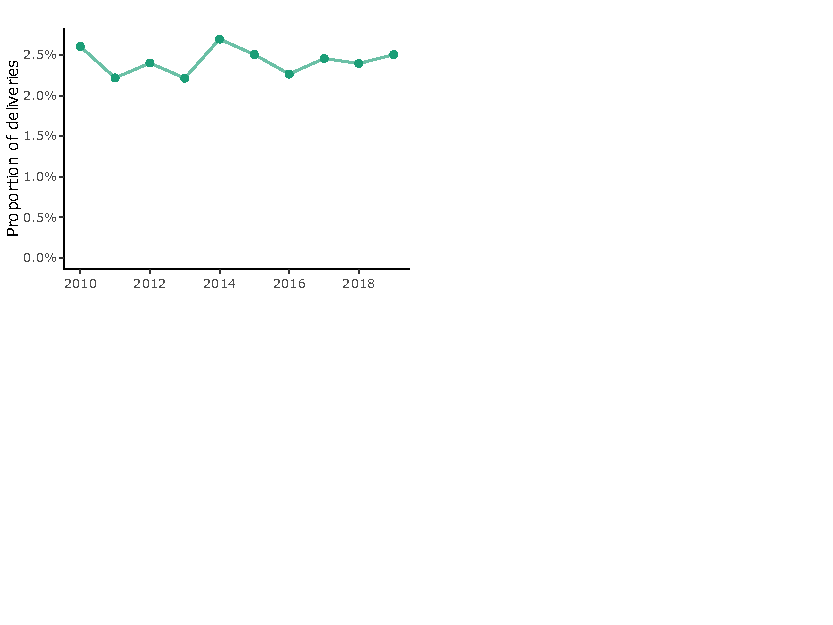
\includegraphics[width=0.9\linewidth,]{01-Deliveries_births_files/figure-latex/plot12-1} \end{center}

\begin{table}[H]
\centering\begingroup\fontsize{10}{12}\selectfont

\resizebox{\linewidth}{!}{
\begin{tabular}[t]{lllllllllll}
\toprule
\textbf{} & \textbf{2011} & \textbf{2012} & \textbf{2013} & \textbf{2014} & \textbf{2015} & \textbf{2016} & \textbf{2017} & \textbf{2018} & \textbf{2019} & \textbf{2020}\\
\midrule
Total births & 8,904 & 8,766 & 8,468 & 8,664 & 8,176 & 8,320 & 8,252 & 7,951 & 8,081 & 7,604\\
\bottomrule
\end{tabular}}
\endgroup{}
\end{table}

\hypertarget{section-13}{%
\section{Number of births by outcome, sex, and year, Nova Scotia, 2011-2020}\label{section-13}}

\begin{table}[H]
\centering
\resizebox{\linewidth}{!}{
\begin{threeparttable}
\begin{tabular}[t]{lrrrrrrrrrr}
\toprule
\textbf{} & \textbf{2011} & \textbf{2012} & \textbf{2013} & \textbf{2014} & \textbf{2015} & \textbf{2016} & \textbf{2017} & \textbf{2018} & \textbf{2019} & \textbf{2020}\\
\midrule
Female live births & 4349 & 4246 & 4090 & 4244 & 3971 & 4082 & 3932 & 3849 & 3931 & 3730\\
Female stillbirths & 23 & 21 & 17 & 23 & 16 & 13 & 23 & 23 & 17 & 12\\
\midrule
\cellcolor[HTML]{E1E1E1}{\textbf{Total Female births}} & \cellcolor[HTML]{E1E1E1}{\textbf{4372}} & \cellcolor[HTML]{E1E1E1}{\textbf{4267}} & \cellcolor[HTML]{E1E1E1}{\textbf{4107}} & \cellcolor[HTML]{E1E1E1}{\textbf{4267}} & \cellcolor[HTML]{E1E1E1}{\textbf{3987}} & \cellcolor[HTML]{E1E1E1}{\textbf{4095}} & \cellcolor[HTML]{E1E1E1}{\textbf{3955}} & \cellcolor[HTML]{E1E1E1}{\textbf{3872}} & \cellcolor[HTML]{E1E1E1}{\textbf{3948}} & \cellcolor[HTML]{E1E1E1}{\textbf{3742}}\\
\midrule
Male live births & 4514 & 4475 & 4344 & 4367 & 4166 & 4212 & 4284 & 4062 & 4113 & 3837\\
Male stillbirths & 16 & 22 & 17 & 27 & 21 & 12 & 13 & 16 & 18 & 24\\
\midrule
\cellcolor[HTML]{E1E1E1}{\textbf{Total Male births}} & \cellcolor[HTML]{E1E1E1}{\textbf{4530}} & \cellcolor[HTML]{E1E1E1}{\textbf{4497}} & \cellcolor[HTML]{E1E1E1}{\textbf{4361}} & \cellcolor[HTML]{E1E1E1}{\textbf{4394}} & \cellcolor[HTML]{E1E1E1}{\textbf{4187}} & \cellcolor[HTML]{E1E1E1}{\textbf{4224}} & \cellcolor[HTML]{E1E1E1}{\textbf{4297}} & \cellcolor[HTML]{E1E1E1}{\textbf{4078}} & \cellcolor[HTML]{E1E1E1}{\textbf{4131}} & \cellcolor[HTML]{E1E1E1}{\textbf{3861}}\\
\midrule
Total live births & 8863 & 8722 & 8434 & 8612 & 8138 & 8294 & 8216 & 7911 & 8046 & 7567\\
Total stillbirths & 41 & 44 & 34 & 52 & 38 & 26 & 36 & 40 & 35 & 37\\
\midrule
\cellcolor[HTML]{E1E1E1}{\textbf{Total births}} & \cellcolor[HTML]{E1E1E1}{\textbf{8904}} & \cellcolor[HTML]{E1E1E1}{\textbf{8766}} & \cellcolor[HTML]{E1E1E1}{\textbf{8468}} & \cellcolor[HTML]{E1E1E1}{\textbf{8664}} & \cellcolor[HTML]{E1E1E1}{\textbf{8176}} & \cellcolor[HTML]{E1E1E1}{\textbf{8320}} & \cellcolor[HTML]{E1E1E1}{\textbf{8252}} & \cellcolor[HTML]{E1E1E1}{\textbf{7951}} & \cellcolor[HTML]{E1E1E1}{\textbf{8081}} & \cellcolor[HTML]{E1E1E1}{\textbf{7604}}\\
\bottomrule
\end{tabular}
\begin{tablenotes}
\item \textit{Note: } 
\item Sex could not be determined in some infants and these infants are not included in the male or female categories.
\item Stillbirth refers to the complete expulsion or extraction from its mother after at least 20 weeks pregnancy, or after attaining a weight of 500 g or more, of a fetus in whom, after such expulsion or extraction, there is no breathing, beating of the heart, pulsation of the umbilical cord, or unmistakable movement of voluntary muscle.
\end{tablenotes}
\end{threeparttable}}
\end{table}

\hypertarget{section-14}{%
\section{Deliveries resulting from assisted reproductive technology, Nova Scotia, 2011-2020}\label{section-14}}

\begin{center}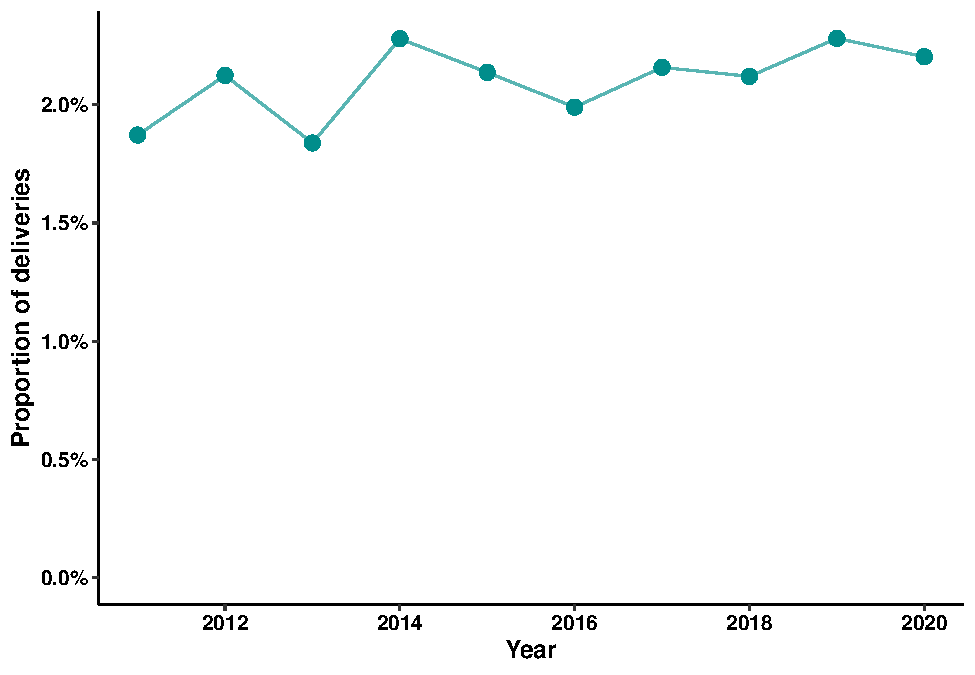
\includegraphics[width=0.9\linewidth,]{01-Deliveries_births_files/figure-latex/plot14-1} \end{center}

\begin{table}[H]
\centering
\resizebox{\linewidth}{!}{
\begin{threeparttable}
\begin{tabular}[t]{lllllllllll}
\toprule
\textbf{ } & \textbf{2011} & \textbf{2012} & \textbf{2013} & \textbf{2014} & \textbf{2015} & \textbf{2016} & \textbf{2017} & \textbf{2018} & \textbf{2019} & \textbf{2020}\\
\midrule
Total deliveries & 8,764 & 8,618 & 8,325 & 8,514 & 8,051 & 8,194 & 8,111 & 7,832 & 7,938 & 7,491\\
Assisted reproduction & 1.9\% & 2.1\% & 1.8\% & 2.3\% & 2.1\% & 2.0\% & 2.2\% & 2.1\% & 2.3\% & 2.2\%\\
\bottomrule
\end{tabular}
\begin{tablenotes}
\item \textit{Note: } 
\item Assisted reproductive technology can include ovulation induction, intracytoplasmic sperm injection (ICSI), embryo transfer, or in vitro fertilization (IVF).
\end{tablenotes}
\end{threeparttable}}
\end{table}

\hypertarget{section-2}{%
\chapter{Perinatal and Infant Mortality}\label{section-2}}

\hypertarget{section-21}{%
\section{Perinatal mortality by year, Nova Scotia, 2011-2020}\label{section-21}}

\begin{center}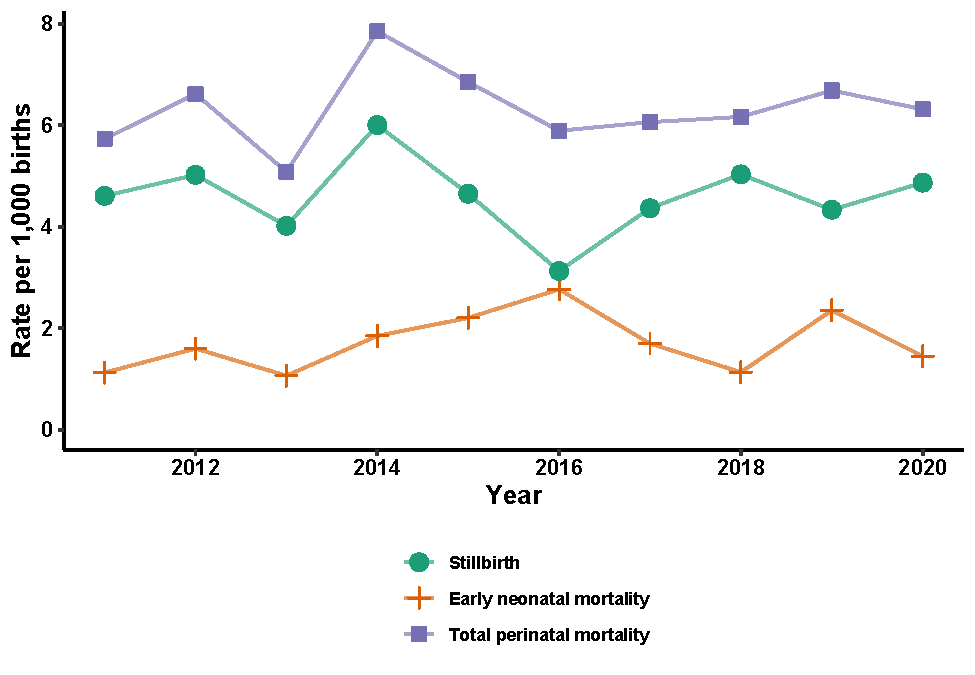
\includegraphics[width=0.9\linewidth,]{02-Perinatal_IM_files/figure-latex/plot21-1} \end{center}

\begin{table}[H]
\centering
\resizebox{\linewidth}{!}{
\begin{threeparttable}
\begin{tabular}[t]{lllllllllll}
\toprule
\textbf{ } & \textbf{2011} & \textbf{2012} & \textbf{2013} & \textbf{2014} & \textbf{2015} & \textbf{2016} & \textbf{2017} & \textbf{2018} & \textbf{2019} & \textbf{2020}\\
\midrule
Total births & 8,904 & 8,766 & 8,468 & 8,664 & 8,176 & 8,320 & 8,252 & 7,951 & 8,081 & 7,604\\
\cellcolor[HTML]{E1E1E1}{\textbf{Rate per 1,000 births}} & \cellcolor[HTML]{E1E1E1}{\textbf{}} & \cellcolor[HTML]{E1E1E1}{\textbf{}} & \cellcolor[HTML]{E1E1E1}{\textbf{}} & \cellcolor[HTML]{E1E1E1}{\textbf{}} & \cellcolor[HTML]{E1E1E1}{\textbf{}} & \cellcolor[HTML]{E1E1E1}{\textbf{}} & \cellcolor[HTML]{E1E1E1}{\textbf{}} & \cellcolor[HTML]{E1E1E1}{\textbf{}} & \cellcolor[HTML]{E1E1E1}{\textbf{}} & \cellcolor[HTML]{E1E1E1}{\textbf{}}\\
Stillbirth & 4.6 & 5.0 & 4.0 & 6.0 & 4.6 & 3.1 & 4.4 & 5.0 & 4.3 & 4.9\\
Early neonatal mortality & 1.1 & 1.6 & 1.1 & 1.8 & 2.2 & 2.8 & 1.7 & 1.1 & 2.4 & 1.4\\
Total perinatal mortality & 5.7 & 6.6 & 5.1 & 7.8 & 6.8 & 5.9 & 6.1 & 6.2 & 6.7 & 6.3\\
\bottomrule
\end{tabular}
\begin{tablenotes}
\item \textit{Note: } 
\item Stillbirth refers to the complete expulsion or extraction from its mother after at least 20 weeks pregnancy, or after attaining a weight of 500 g or more, of a fetus in whom, after such expulsion or extraction, there is no breathing, beating of the heart, pulsation of the umbilical cord, or unmistakable movement of voluntary muscle. Early neonatal mortality refers to the death of a liveborn infant, occurring up to the sixth completed day of life (6 days, 23 hours and 59 minutes). Perinatal mortality includes both stillbirths and early neonatal deaths.
\end{tablenotes}
\end{threeparttable}}
\end{table}

\hypertarget{section-22}{%
\section{Infant mortality by year, Nova Scotia, 2011-2020}\label{section-22}}

\begin{center}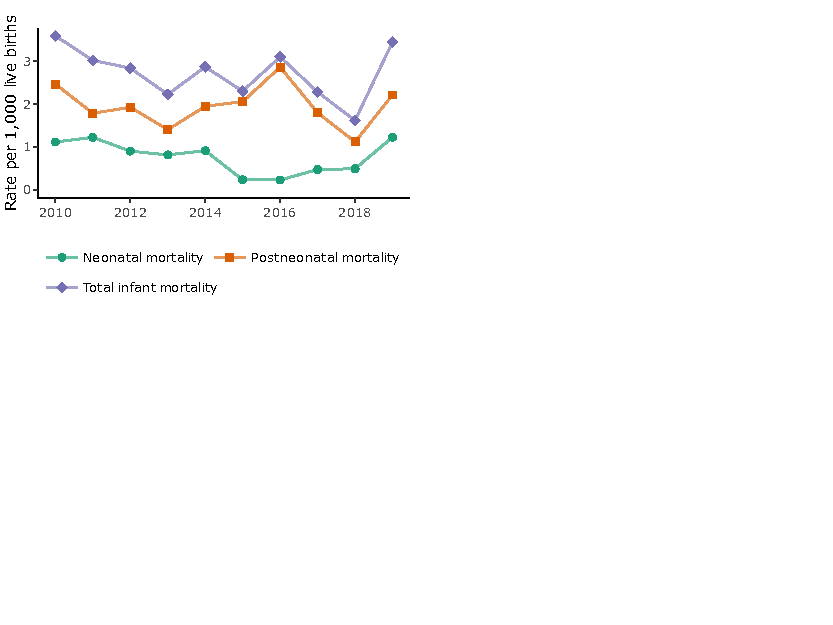
\includegraphics[width=0.9\linewidth,]{02-Perinatal_IM_files/figure-latex/plot22-1} \end{center}

\begin{table}[H]
\centering
\resizebox{\linewidth}{!}{
\begin{threeparttable}
\begin{tabular}[t]{lllllllllll}
\toprule
\textbf{ } & \textbf{2011} & \textbf{2012} & \textbf{2013} & \textbf{2014} & \textbf{2015} & \textbf{2016} & \textbf{2017} & \textbf{2018} & \textbf{2019} & \textbf{2020}\\
\midrule
Total live births & 8,863 & 8,722 & 8,434 & 8,612 & 8,138 & 8,294 & 8,216 & 7,911 & 8,046 & 7,567\\
\cellcolor[HTML]{E1E1E1}{\textbf{Rate per 1,000 births}} & \cellcolor[HTML]{E1E1E1}{\textbf{}} & \cellcolor[HTML]{E1E1E1}{\textbf{}} & \cellcolor[HTML]{E1E1E1}{\textbf{}} & \cellcolor[HTML]{E1E1E1}{\textbf{}} & \cellcolor[HTML]{E1E1E1}{\textbf{}} & \cellcolor[HTML]{E1E1E1}{\textbf{}} & \cellcolor[HTML]{E1E1E1}{\textbf{}} & \cellcolor[HTML]{E1E1E1}{\textbf{}} & \cellcolor[HTML]{E1E1E1}{\textbf{}} & \cellcolor[HTML]{E1E1E1}{\textbf{}}\\
Neonatal mortality & 1.9 & 2.3 & 1.7 & 2.4 & 2.6 & 2.9 & 2.3 & 1.4 & 3.0 & 2.1\\
Postneonatal mortality & 0.3 & 0.7 & 0.9 & 1.4 & 0.5 & 1.1 & 0.7 & 1.3 & 1.5 & 1.3\\
Total infant mortality & 2.3 & 3.0 & 2.6 & 3.8 & 3.1 & 4.0 & 3.0 & 2.7 & 4.5 & 3.4\\
\bottomrule
\end{tabular}
\begin{tablenotes}
\item \textit{Note: } 
\item Neonatal mortality refers to the death of a liveborn infant, occurring up to the $27^{th}$ completed day of life (27 days, 23 hours and 59 minutes). Postneonatal mortality denotes the death of a liveborn infant weighing 500 g or more at birth, occurring from 28 days to 1 year of life. Infant mortality encompasses both neonatal and postneonatal mortality, that is, the death of a liveborn infant occurring within the first year of life.
\end{tablenotes}
\end{threeparttable}}
\end{table}

\hypertarget{section-3}{%
\chapter{Determinants of Maternal, Fetal, and Infant Health}\label{section-3}}

\hypertarget{section-31}{%
\section{Maternal age by year, Nova Scotia, 2011-2020}\label{section-31}}

\begin{center}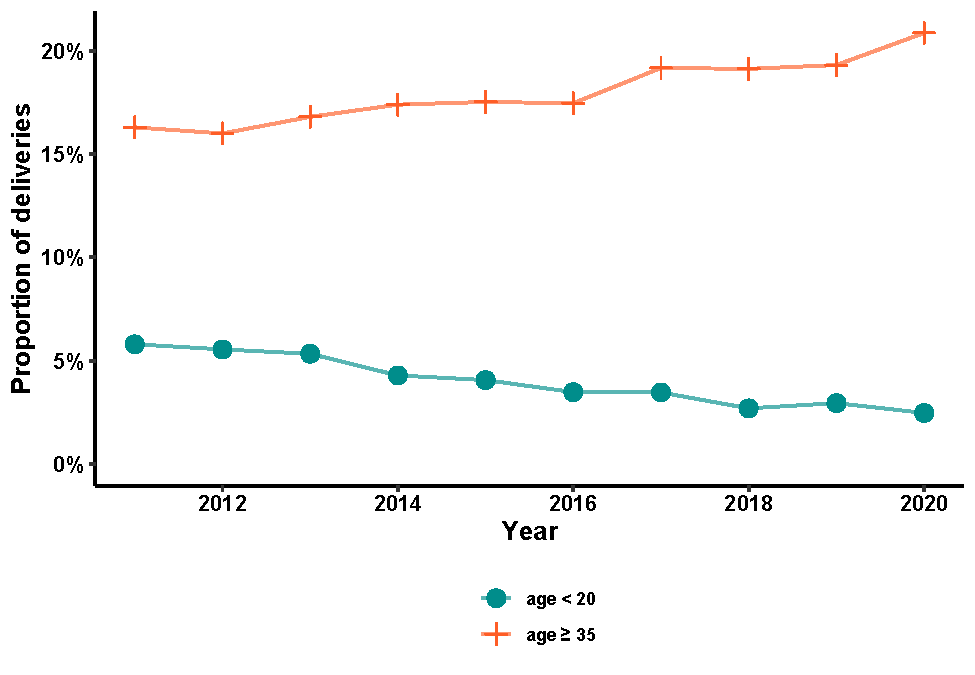
\includegraphics[width=0.9\linewidth,]{03-Determinants_MFIH_files/figure-latex/plot31-1} \end{center}

\begin{table}[H]
\centering
\resizebox{\linewidth}{!}{
\begin{tabular}[t]{lllllllllll}
\toprule
\textbf{} & \textbf{2011} & \textbf{2012} & \textbf{2013} & \textbf{2014} & \textbf{2015} & \textbf{2016} & \textbf{2017} & \textbf{2018} & \textbf{2019} & \textbf{2020}\\
\midrule
Total deliveries & 8,764 & 8,618 & 8,325 & 8,514 & 8,051 & 8,194 & 8,111 & 7,832 & 7,938 & 7,491\\
age < 20 & 5.8$\%$ & 5.5$\%$ & 5.3$\%$ & 4.3$\%$ & 4.1$\%$ & 3.5$\%$ & 3.5$\%$ & 2.7$\%$ & 2.9$\%$ & 2.5$\%$\\
age $\geq$ 35 & 16.3$\%$ & 16.0$\%$ & 16.8$\%$ & 17.4$\%$ & 17.5$\%$ & 17.5$\%$ & 19.2$\%$ & 19.1$\%$ & 19.3$\%$ & 20.9$\%$\\
\bottomrule
\end{tabular}}
\end{table}

\hypertarget{section-32}{%
\section{Maternal age by parity and year, Nova Scotia, 2011-2020}\label{section-32}}

\begin{center}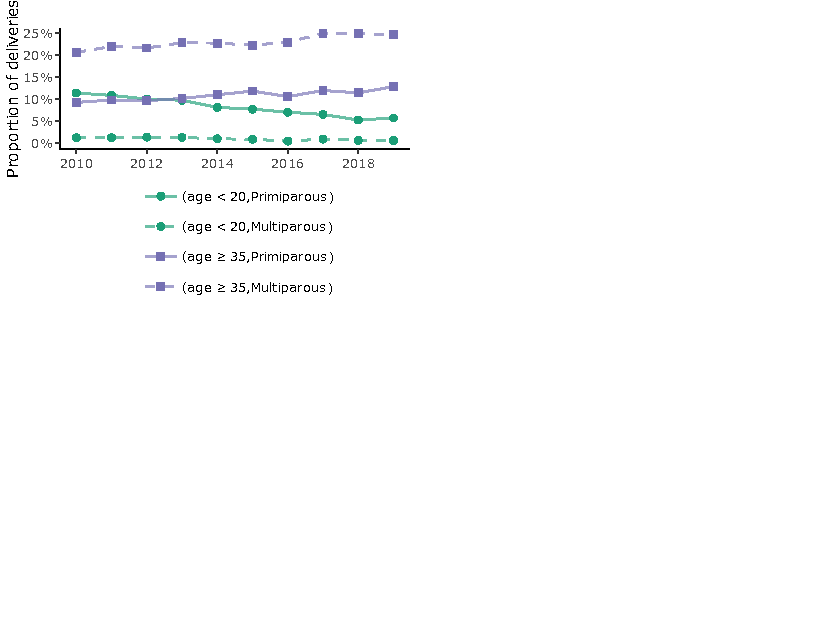
\includegraphics[width=0.9\linewidth,]{03-Determinants_MFIH_files/figure-latex/plot32-1} \end{center}

\begin{table}[H]
\centering
\resizebox{\linewidth}{!}{
\begin{tabular}[t]{lllllllllll}
\toprule
\textbf{} & \textbf{2011} & \textbf{2012} & \textbf{2013} & \textbf{2014} & \textbf{2015} & \textbf{2016} & \textbf{2017} & \textbf{2018} & \textbf{2019} & \textbf{2020}\\
\midrule
\cellcolor[HTML]{E1E1E1}{\textbf{Primiparous}} & \cellcolor[HTML]{E1E1E1}{\textbf{}} & \cellcolor[HTML]{E1E1E1}{\textbf{}} & \cellcolor[HTML]{E1E1E1}{\textbf{}} & \cellcolor[HTML]{E1E1E1}{\textbf{}} & \cellcolor[HTML]{E1E1E1}{\textbf{}} & \cellcolor[HTML]{E1E1E1}{\textbf{}} & \cellcolor[HTML]{E1E1E1}{\textbf{}} & \cellcolor[HTML]{E1E1E1}{\textbf{}} & \cellcolor[HTML]{E1E1E1}{\textbf{}} & \cellcolor[HTML]{E1E1E1}{\textbf{}}\\
Total deliveries & 4,027 & 4,036 & 3,813 & 3,797 & 3,556 & 3,606 & 3,565 & 3,326 & 3,489 & 3,254\\
age < 20 & 11.1$\%$ & 10.2$\%$ & 10.0$\%$ & 8.3$\%$ & 8.0$\%$ & 7.2$\%$ & 6.6$\%$ & 5.4$\%$ & 5.9$\%$ & 4.9$\%$\\
age $\geq$ 35 & 9.6$\%$ & 9.7$\%$ & 9.8$\%$ & 10.7$\%$ & 11.7$\%$ & 10.3$\%$ & 11.8$\%$ & 11.3$\%$ & 12.5$\%$ & 13.9$\%$\\
\cellcolor[HTML]{E1E1E1}{\textbf{Multiparous}} & \cellcolor[HTML]{E1E1E1}{\textbf{}} & \cellcolor[HTML]{E1E1E1}{\textbf{}} & \cellcolor[HTML]{E1E1E1}{\textbf{}} & \cellcolor[HTML]{E1E1E1}{\textbf{}} & \cellcolor[HTML]{E1E1E1}{\textbf{}} & \cellcolor[HTML]{E1E1E1}{\textbf{}} & \cellcolor[HTML]{E1E1E1}{\textbf{}} & \cellcolor[HTML]{E1E1E1}{\textbf{}} & \cellcolor[HTML]{E1E1E1}{\textbf{}} & \cellcolor[HTML]{E1E1E1}{\textbf{}}\\
Total deliveries & 4,737 & 4,581 & 4,510 & 4,717 & 4,494 & 4,587 & 4,545 & 4,505 & 4,448 & 4,237\\
age < 20 & 1.3$\%$ & 1.5$\%$ & 1.4$\%$ & 1.0$\%$ & 1.0$\%$ & 0.5$\%$ & 1.0$\%$ & 0.7$\%$ & 0.6$\%$ & 0.6$\%$\\
age $\geq$ 35 & 22.0$\%$ & 21.5$\%$ & 22.7$\%$ & 22.8$\%$ & 22.1$\%$ & 23.1$\%$ & 25.0$\%$ & 24.9$\%$ & 24.6$\%$ & 26.2$\%$\\
\bottomrule
\end{tabular}}
\end{table}

\hypertarget{section-33}{%
\section{Maternal parity by year, Nova Scotia, 2011-2020}\label{section-33}}

\begin{center}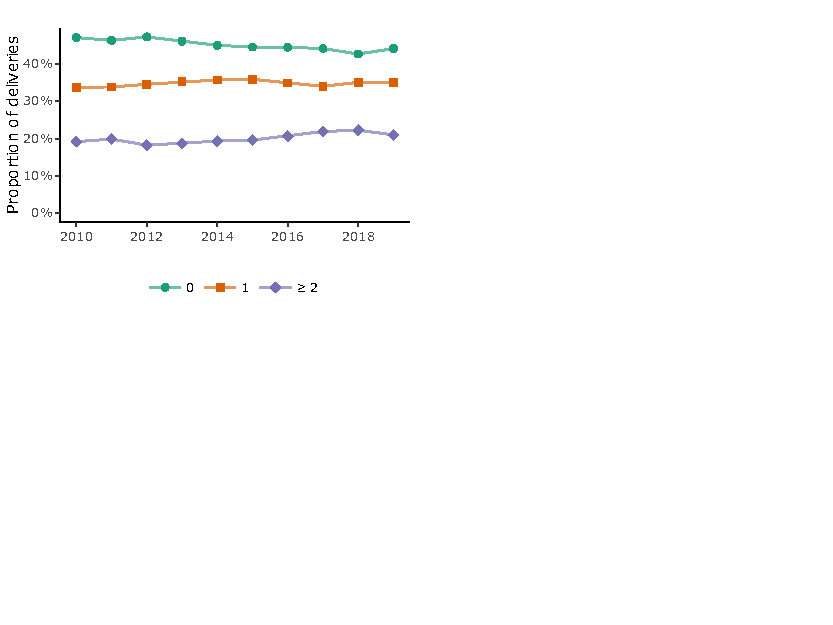
\includegraphics[width=0.9\linewidth,]{03-Determinants_MFIH_files/figure-latex/plot33-1} \end{center}

\begin{table}[H]
\centering
\resizebox{\linewidth}{!}{
\begin{threeparttable}
\begin{tabular}[t]{lllllllllll}
\toprule
\textbf{} & \textbf{2011} & \textbf{2012} & \textbf{2013} & \textbf{2014} & \textbf{2015} & \textbf{2016} & \textbf{2017} & \textbf{2018} & \textbf{2019} & \textbf{2020}\\
\midrule
Total deliveries\textsuperscript{a} & 8,764 & 8,617 & 8,323 & 8,514 & 8,050 & 8,193 & 8,110 & 7,831 & 7,937 & 7,491\\
0 & 45.9$\%$ & 46.8$\%$ & 45.8$\%$ & 44.6$\%$ & 44.2$\%$ & 44.0$\%$ & 44.0$\%$ & 42.5$\%$ & 44.0$\%$ & 43.4$\%$\\
1 & 34.2$\%$ & 34.9$\%$ & 35.5$\%$ & 36.1$\%$ & 36.1$\%$ & 35.2$\%$ & 34.2$\%$ & 35.2$\%$ & 35.2$\%$ & 35.4$\%$\\
$\geq$ 2 & 19.8$\%$ & 18.2$\%$ & 18.7$\%$ & 19.3$\%$ & 19.7$\%$ & 20.8$\%$ & 21.9$\%$ & 22.4$\%$ & 20.9$\%$ & 21.2$\%$\\
\bottomrule
\end{tabular}
\begin{tablenotes}
\item[a] With known parity.
\end{tablenotes}
\end{threeparttable}}
\end{table}

\hypertarget{section-34}{%
\section{Maternal partner status by year, Nova Scotia, 2011-2020}\label{section-34}}

\begin{center}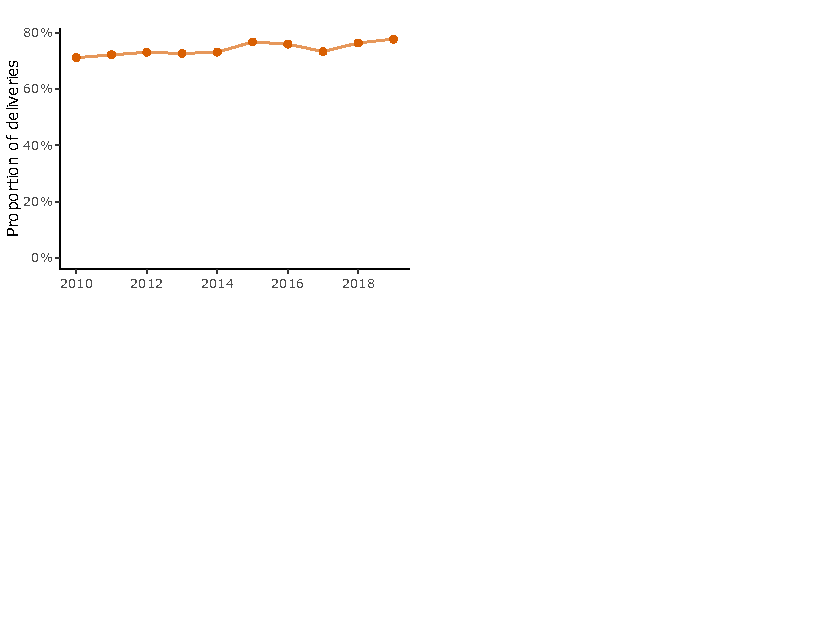
\includegraphics[width=0.9\linewidth,]{03-Determinants_MFIH_files/figure-latex/plot34-1} \end{center}

\begin{table}[H]
\centering
\resizebox{\linewidth}{!}{
\begin{threeparttable}
\begin{tabular}[t]{lllllllllll}
\toprule
\textbf{} & \textbf{2011} & \textbf{2012} & \textbf{2013} & \textbf{2014} & \textbf{2015} & \textbf{2016} & \textbf{2017} & \textbf{2018} & \textbf{2019} & \textbf{2020}\\
\midrule
Total deliveries\textsuperscript{a} & 8,320 & 8,090 & 7,734 & 7,807 & 7,160 & 7,424 & 7,430 & 7,174 & 7,315 & 6,806\\
Partnered & 72.2$\%$ & 73.2$\%$ & 72.5$\%$ & 73.2$\%$ & 76.8$\%$ & 76.0$\%$ & 73.6$\%$ & 76.4$\%$ & 77.7$\%$ & 81.2$\%$\\
Unknown & 5.3$\%$ & 6.5$\%$ & 7.6$\%$ & 9.1$\%$ & 12.4$\%$ & 10.4$\%$ & 9.2$\%$ & 9.2$\%$ & 8.5$\%$ & 10.1$\%$\\
\bottomrule
\end{tabular}
\begin{tablenotes}
\item \textit{Note: } 
\item Partnered denotes women who are married or in a common-law relationship.
\item[a] With known partner status.
\end{tablenotes}
\end{threeparttable}}
\end{table}

\hypertarget{section-35}{%
\section{Maternal smoking during pregnancy by year, Nova Scotia, 2011-2020}\label{section-35}}

\begin{center}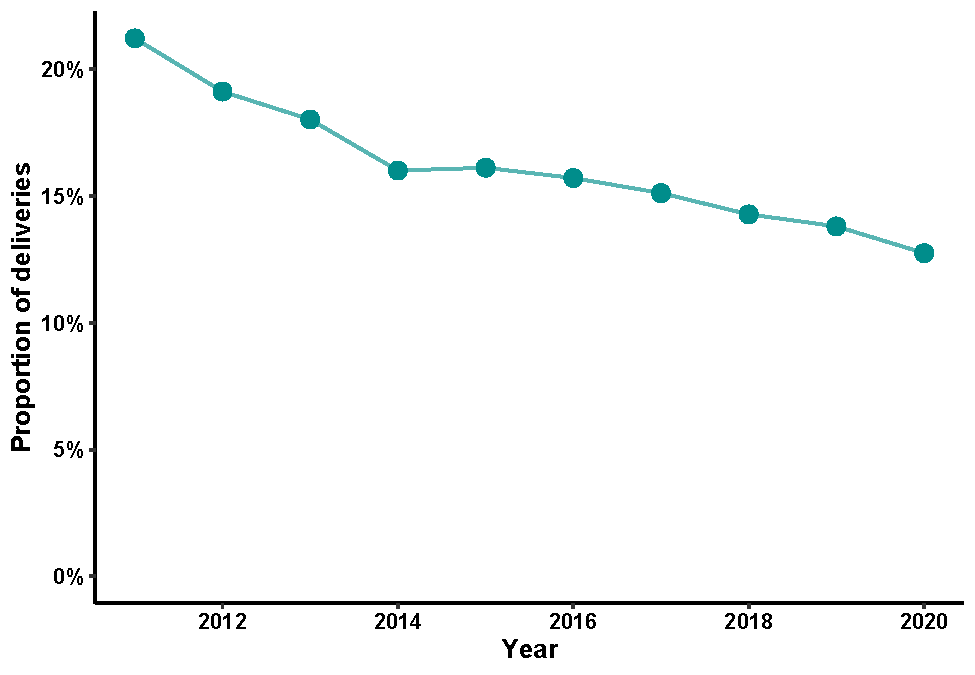
\includegraphics[width=0.9\linewidth,]{03-Determinants_MFIH_files/figure-latex/plot35-1} \end{center}

\begin{table}[H]
\centering
\resizebox{\linewidth}{!}{
\begin{threeparttable}
\begin{tabular}[t]{lllllllllll}
\toprule
\textbf{} & \textbf{2011} & \textbf{2012} & \textbf{2013} & \textbf{2014} & \textbf{2015} & \textbf{2016} & \textbf{2017} & \textbf{2018} & \textbf{2019} & \textbf{2020}\\
\midrule
Total deliveries\textsuperscript{a} & 8,713 & 8,541 & 8,219 & 8,441 & 8,018 & 8,154 & 8,044 & 7,802 & 7,911 & 7,467\\
Smoking & 21.2$\%$ & 19.1$\%$ & 18.0$\%$ & 16.0$\%$ & 16.1$\%$ & 15.7$\%$ & 15.1$\%$ & 14.3$\%$ & 13.8$\%$ & 12.7$\%$\\
\bottomrule
\end{tabular}
\begin{tablenotes}
\item[a] With known smoking status.
\end{tablenotes}
\end{threeparttable}}
\end{table}

\hypertarget{section-36}{%
\section{Reduction in amount smoked among women who smoked at their first prenatal visit by year, Nova Scotia, 2011-2020}\label{section-36}}

\begin{center}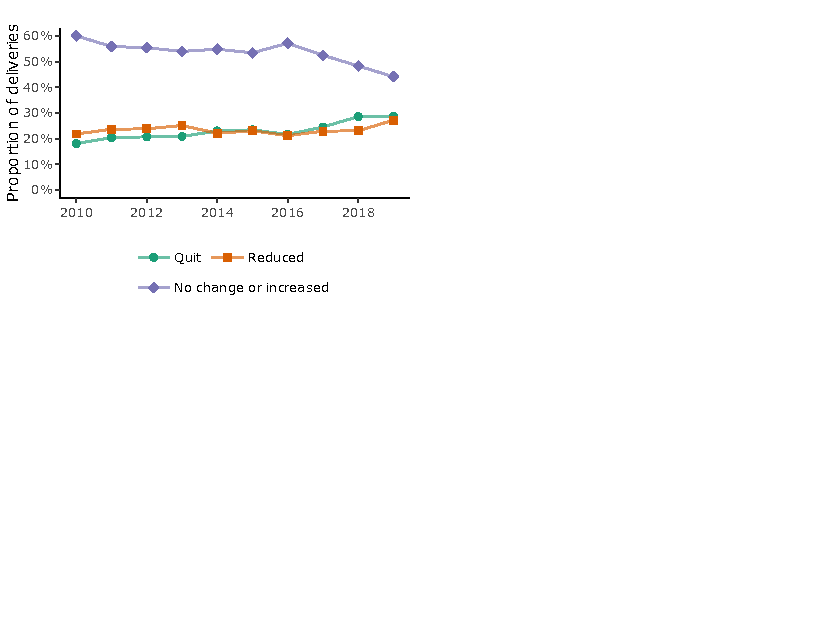
\includegraphics[width=0.9\linewidth,]{03-Determinants_MFIH_files/figure-latex/plot36-1} \end{center}

\begin{table}[H]
\centering
\resizebox{\linewidth}{!}{
\begin{threeparttable}
\begin{tabular}[t]{lllllllllll}
\toprule
\textbf{} & \textbf{2011} & \textbf{2012} & \textbf{2013} & \textbf{2014} & \textbf{2015} & \textbf{2016} & \textbf{2017} & \textbf{2018} & \textbf{2019} & \textbf{2020}\\
\midrule
Total deliveries\textsuperscript{a} & 1,173 & 1,031 & 912 & 843 & 803 & 821 & 761 & 749 & 702 & 614\\
Quit & 20.3$\%$ & 20.8$\%$ & 20.6$\%$ & 23.1$\%$ & 23.2$\%$ & 21.7$\%$ & 24.7$\%$ & 28.4$\%$ & 28.2$\%$ & 26.9$\%$\\
Reduced & 23.6$\%$ & 23.7$\%$ & 25.0$\%$ & 21.6$\%$ & 23.5$\%$ & 21.1$\%$ & 22.7$\%$ & 23.5$\%$ & 27.4$\%$ & 26.7$\%$\\
No change or increased & 56.1$\%$ & 55.6$\%$ & 54.4$\%$ & 55.3$\%$ & 53.3$\%$ & 57.2$\%$ & 52.6$\%$ & 48.1$\%$ & 44.4$\%$ & 46.4$\%$\\
\bottomrule
\end{tabular}
\begin{tablenotes}
\item[a] Among women who were known to be smokers at the time of their first prenatal visit, and for whom amount smoked was known at both the first prenatal visit and at delivery.
\end{tablenotes}
\end{threeparttable}}
\end{table}

\hypertarget{section-37}{%
\section{Missing information about smoking in pregnancy by year, Nova Scotia, 2011-2020}\label{section-37}}

\begin{table}[H]
\centering
\resizebox{\linewidth}{!}{
\begin{tabular}[t]{lllllllllll}
\toprule
\textbf{} & \textbf{2011} & \textbf{2012} & \textbf{2013} & \textbf{2014} & \textbf{2015} & \textbf{2016} & \textbf{2017} & \textbf{2018} & \textbf{2019} & \textbf{2020}\\
\midrule
\cellcolor[HTML]{E1E1E1}{\textbf{Pre-pregnancy}} & \cellcolor[HTML]{E1E1E1}{\textbf{}} & \cellcolor[HTML]{E1E1E1}{\textbf{}} & \cellcolor[HTML]{E1E1E1}{\textbf{}} & \cellcolor[HTML]{E1E1E1}{\textbf{}} & \cellcolor[HTML]{E1E1E1}{\textbf{}} & \cellcolor[HTML]{E1E1E1}{\textbf{}} & \cellcolor[HTML]{E1E1E1}{\textbf{}} & \cellcolor[HTML]{E1E1E1}{\textbf{}} & \cellcolor[HTML]{E1E1E1}{\textbf{}} & \cellcolor[HTML]{E1E1E1}{\textbf{}}\\
Missing amount & 7.2\% & 7.0\% & 6.5\% & 6.6\% & 5.5\% & 5.1\% & 5.2\% & 4.0\% & 5.0\% & 4.1\%\\
No information & 3.8\% & 4.0\% & 4.6\% & 4.5\% & 3.7\% & 4.2\% & 3.6\% & 2.3\% & 2.7\% & 1.1\%\\
\cellcolor[HTML]{E1E1E1}{\textbf{First visit}} & \cellcolor[HTML]{E1E1E1}{\textbf{}} & \cellcolor[HTML]{E1E1E1}{\textbf{}} & \cellcolor[HTML]{E1E1E1}{\textbf{}} & \cellcolor[HTML]{E1E1E1}{\textbf{}} & \cellcolor[HTML]{E1E1E1}{\textbf{}} & \cellcolor[HTML]{E1E1E1}{\textbf{}} & \cellcolor[HTML]{E1E1E1}{\textbf{}} & \cellcolor[HTML]{E1E1E1}{\textbf{}} & \cellcolor[HTML]{E1E1E1}{\textbf{}} & \cellcolor[HTML]{E1E1E1}{\textbf{}}\\
Missing amount & 4.1\% & 3.5\% & 3.6\% & 3.4\% & 3.0\% & 2.7\% & 2.9\% & 2.5\% & 2.4\% & 3.0\%\\
No information & 4.0\% & 4.2\% & 4.5\% & 4.5\% & 3.6\% & 4.2\% & 3.5\% & 2.5\% & 3.0\% & 1.3\%\\
\cellcolor[HTML]{E1E1E1}{\textbf{Delivery}} & \cellcolor[HTML]{E1E1E1}{\textbf{}} & \cellcolor[HTML]{E1E1E1}{\textbf{}} & \cellcolor[HTML]{E1E1E1}{\textbf{}} & \cellcolor[HTML]{E1E1E1}{\textbf{}} & \cellcolor[HTML]{E1E1E1}{\textbf{}} & \cellcolor[HTML]{E1E1E1}{\textbf{}} & \cellcolor[HTML]{E1E1E1}{\textbf{}} & \cellcolor[HTML]{E1E1E1}{\textbf{}} & \cellcolor[HTML]{E1E1E1}{\textbf{}} & \cellcolor[HTML]{E1E1E1}{\textbf{}}\\
Missing amount & 2.5\% & 2.5\% & 2.6\% & 2.2\% & 2.3\% & 2.3\% & 2.1\% & 1.6\% & 1.4\% & 1.5\%\\
No information & 1.1\% & 1.7\% & 1.9\% & 1.3\% & 0.8\% & 0.9\% & 1.4\% & 1.0\% & 1.1\% & 0.7\%\\
\bottomrule
\end{tabular}}
\end{table}

\hypertarget{section-38}{%
\section{Cannabis use recorded during pregnancy by year, Nova Scotia, 2011-2020}\label{section-38}}

\begin{center}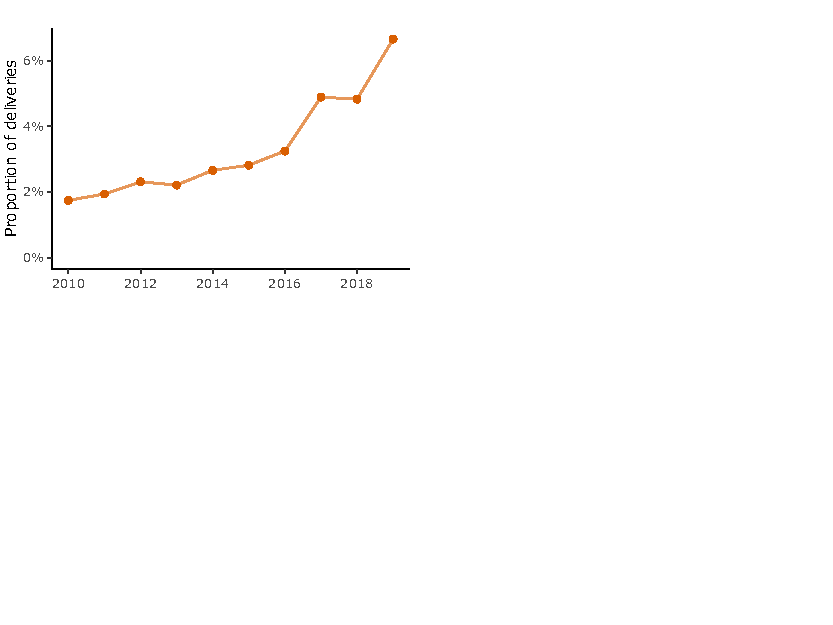
\includegraphics[width=0.9\linewidth,]{03-Determinants_MFIH_files/figure-latex/plot38-1} \end{center}

\begin{table}[H]
\centering
\resizebox{\linewidth}{!}{
\begin{threeparttable}
\begin{tabular}[t]{lllllllllll}
\toprule
\textbf{} & \textbf{2011} & \textbf{2012} & \textbf{2013} & \textbf{2014} & \textbf{2015} & \textbf{2016} & \textbf{2017} & \textbf{2018} & \textbf{2019} & \textbf{2020}\\
\midrule
Total deliveries & 8,764 & 8,618 & 8,325 & 8,514 & 8,051 & 8,194 & 8,111 & 7,832 & 7,938 & 7,491\\
Reported cannabis & 2.0\% & 2.3\% & 2.3\% & 2.7\% & 2.8\% & 3.3\% & 4.9\% & 4.9\% & 6.7\% & 8.2\%\\
\bottomrule
\end{tabular}
\begin{tablenotes}
\item \textit{Note: } 
\item If recorded on the Nova Scotia Prenatal Record.
\end{tablenotes}
\end{threeparttable}}
\end{table}

\hypertarget{section-39}{%
\section{Maternal opioid agonist maintenance therapy during pregnancy by year, Nova Scotia, 2011-2020}\label{section-39}}

\begin{center}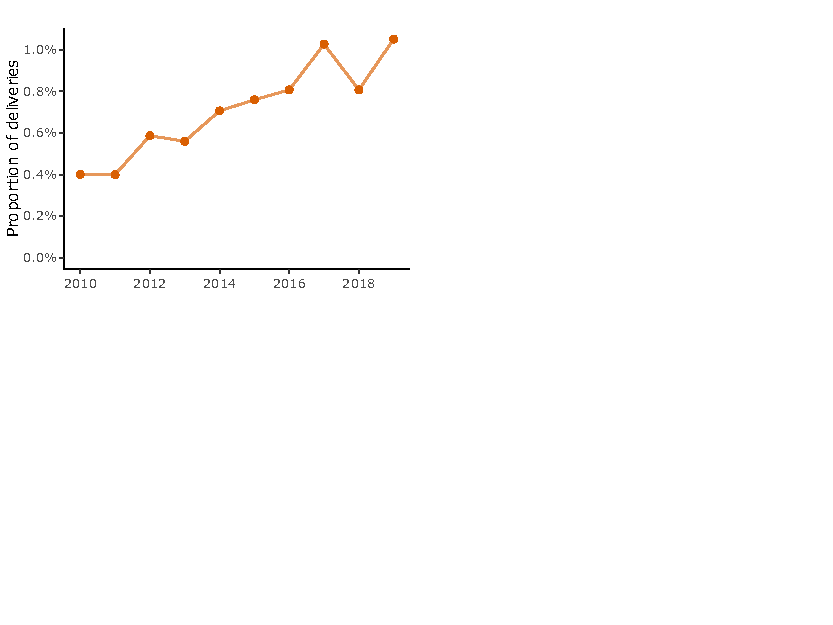
\includegraphics[width=0.9\linewidth,]{03-Determinants_MFIH_files/figure-latex/plot39-1} \end{center}

\begin{table}[H]
\centering
\resizebox{\linewidth}{!}{
\begin{threeparttable}
\begin{tabular}[t]{lllllllllll}
\toprule
\textbf{} & \textbf{2011} & \textbf{2012} & \textbf{2013} & \textbf{2014} & \textbf{2015} & \textbf{2016} & \textbf{2017} & \textbf{2018} & \textbf{2019} & \textbf{2020}\\
\midrule
Total deliveries & 8,764 & 8,619 & 8,325 & 8,514 & 8,051 & 8,194 & 8,111 & 7,832 & 7,938 & 7,491\\
Opioid agonist & 0.40\% & 0.60\% & 0.55\% & 0.70\% & 0.75\% & 0.82\% & 1.04\% & 0.83\% & 1.06\% & 0.91\%\\
\bottomrule
\end{tabular}
\begin{tablenotes}
\item \textit{Note: } 
\item Methadone use as recorded on the Nova Scotia Prenatal Record.
\end{tablenotes}
\end{threeparttable}}
\end{table}

\hypertarget{section-310}{%
\section{Pre-pregnancy body mass index by year, Nova Scotia, 2011-2020}\label{section-310}}

\begin{center}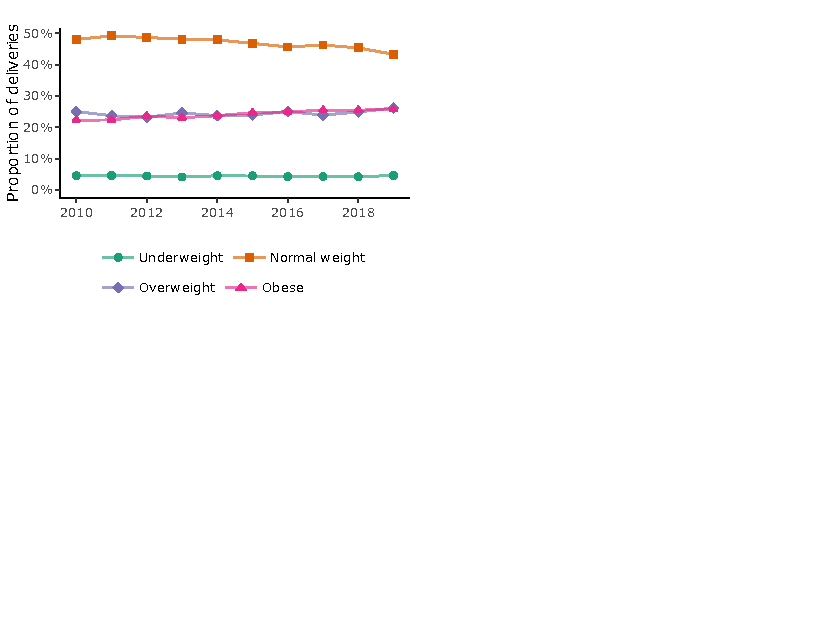
\includegraphics[width=0.9\linewidth,]{03-Determinants_MFIH_files/figure-latex/plot310-1} \end{center}

\begin{table}[H]
\centering
\resizebox{\linewidth}{!}{
\begin{threeparttable}
\begin{tabular}[t]{lllllllllll}
\toprule
\textbf{} & \textbf{2011} & \textbf{2012} & \textbf{2013} & \textbf{2014} & \textbf{2015} & \textbf{2016} & \textbf{2017} & \textbf{2018} & \textbf{2019} & \textbf{2020}\\
\midrule
Total deliveries\textsuperscript{a} & 7,071 & 7,114 & 6,925 & 7,059 & 6,731 & 6,916 & 6,978 & 6,803 & 6,810 & 6,516\\
Underweight & 4.8$\%$ & 4.5$\%$ & 4.2$\%$ & 4.6$\%$ & 4.5$\%$ & 4.4$\%$ & 4.4$\%$ & 4.2$\%$ & 4.7$\%$ & 4.0$\%$\\
Normal weight & 49.2$\%$ & 48.7$\%$ & 48.3$\%$ & 47.9$\%$ & 46.8$\%$ & 45.6$\%$ & 46.5$\%$ & 45.3$\%$ & 43.4$\%$ & 44.4$\%$\\
Overweight & 23.8$\%$ & 23.2$\%$ & 24.6$\%$ & 23.8$\%$ & 24.1$\%$ & 25.1$\%$ & 23.7$\%$ & 25.0$\%$ & 26.1$\%$ & 26.1$\%$\\
Obese & 22.3$\%$ & 23.5$\%$ & 22.9$\%$ & 23.7$\%$ & 24.6$\%$ & 24.9$\%$ & 25.4$\%$ & 25.5$\%$ & 25.7$\%$ & 25.5$\%$\\
\bottomrule
\multicolumn{11}{l}{\rule{0pt}{1em}\textsuperscript{a} With known pre-pregnancy weight and height.}\\
\end{tabular}
\begin{tablenotes}
\item \textit{Note: } 
\item Body mass index (BMI) is calculated as weight in kilograms divided by the square of height in metres: Underweight, < 18.5 kg/$m^{2}$ ; Normal weight, 18.5 to 24.9 kg/$m^{2}$ ; Overweight, 25 to 29.9 kg/$m^{2}$ ; Obese, $\geq 30$ kg/$m^{2}$.
\end{tablenotes}
\end{threeparttable}}
\end{table}

\hypertarget{section-311}{%
\section{Pre-pregnancy obesity class by year, Nova Scotia, 2011-2020}\label{section-311}}

\begin{center}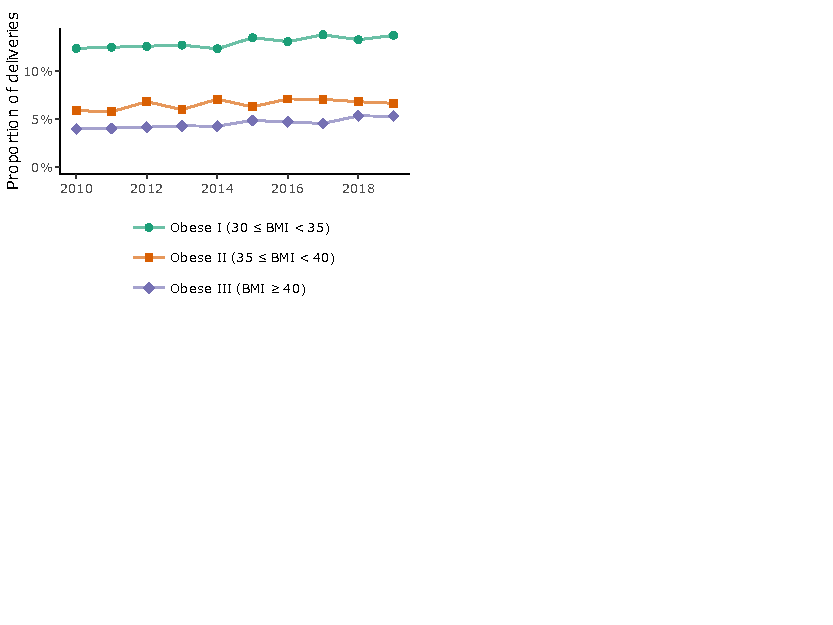
\includegraphics[width=0.9\linewidth,]{03-Determinants_MFIH_files/figure-latex/plot311-1} \end{center}

\begin{table}[H]
\centering
\resizebox{\linewidth}{!}{
\begin{threeparttable}
\begin{tabular}[t]{lllllllllll}
\toprule
\textbf{} & \textbf{2011} & \textbf{2012} & \textbf{2013} & \textbf{2014} & \textbf{2015} & \textbf{2016} & \textbf{2017} & \textbf{2018} & \textbf{2019} & \textbf{2020}\\
\midrule
Total deliveries\textsuperscript{a} & 7,071 & 7,114 & 6,925 & 7,059 & 6,731 & 6,916 & 6,978 & 6,803 & 6,810 & 6,516\\
Obese I (30 $\leq$ BMI < 35) & 12.5$\%$ & 12.6$\%$ & 12.7$\%$ & 12.3$\%$ & 13.5$\%$ & 13.1$\%$ & 13.8$\%$ & 13.4$\%$ & 13.8$\%$ & 13.4$\%$\\
Obese II (35 $\leq$ BMI < 40) & 5.7$\%$ & 6.8$\%$ & 6.1$\%$ & 7.1$\%$ & 6.3$\%$ & 7.1$\%$ & 7.0$\%$ & 6.8$\%$ & 6.6$\%$ & 6.9$\%$\\
Obese III (BMI $\geq$ 40) & 4.1$\%$ & 4.2$\%$ & 4.2$\%$ & 4.2$\%$ & 4.8$\%$ & 4.7$\%$ & 4.6$\%$ & 5.4$\%$ & 5.3$\%$ & 5.3$\%$\\
\bottomrule
\end{tabular}
\begin{tablenotes}
\item[a] With known pre-pregnancy status.
\end{tablenotes}
\end{threeparttable}}
\end{table}

\hypertarget{section-312}{%
\section{Gestational weight gain according to recommendations by year, Nova Scotia, 2011-2020}\label{section-312}}

\begin{center}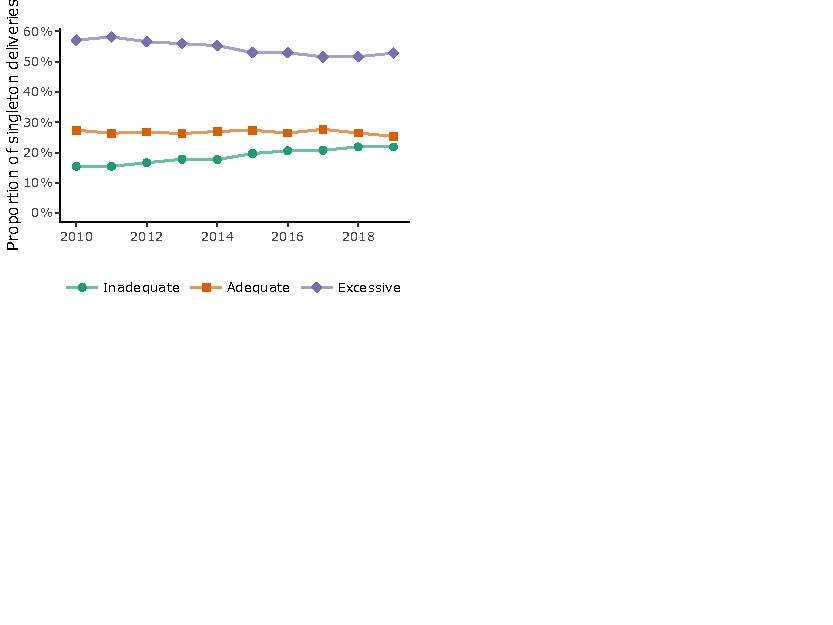
\includegraphics[width=0.9\linewidth,]{03-Determinants_MFIH_files/figure-latex/plot312-1} \end{center}

\begin{table}[H]
\centering
\resizebox{\linewidth}{!}{
\begin{threeparttable}
\begin{tabular}[t]{lllllllllll}
\toprule
\textbf{} & \textbf{2011} & \textbf{2012} & \textbf{2013} & \textbf{2014} & \textbf{2015} & \textbf{2016} & \textbf{2017} & \textbf{2018} & \textbf{2019} & \textbf{2020}\\
\midrule
Total deliveries\textsuperscript{a} & 6,185 & 6,151 & 6,060 & 6,068 & 5,699 & 5,773 & 5,657 & 5,598 & 5,636 & 5,645\\
Inadequate & 15.4$\%$ & 16.6$\%$ & 17.8$\%$ & 17.7$\%$ & 19.7$\%$ & 20.6$\%$ & 20.7$\%$ & 21.9$\%$ & 21.8$\%$ & 20.2$\%$\\
Adequate & 26.4$\%$ & 26.8$\%$ & 26.3$\%$ & 27.0$\%$ & 27.3$\%$ & 26.5$\%$ & 27.6$\%$ & 26.4$\%$ & 25.3$\%$ & 26.1$\%$\\
Excessive & 58.1$\%$ & 56.6$\%$ & 56.0$\%$ & 55.3$\%$ & 53.1$\%$ & 52.9$\%$ & 51.7$\%$ & 51.8$\%$ & 52.8$\%$ & 53.7$\%$\\
\bottomrule
\end{tabular}
\begin{tablenotes}
\item \textit{Note: } 
\item Gestational weight gain according to recommendations made by Health Canada. See section 3.13 for the amounts that are recommended according to pre-pregnancy BMI category.
\item[a] Singleton deliveries with known pre-pregnancy and delivery weights and height.
\end{tablenotes}
\end{threeparttable}}
\end{table}

\hypertarget{section-313}{%
\section{Gestational weight gain by pre-pregnancy body mass index and year, Nova Scotia, 2011-2020}\label{section-313}}

\begin{center}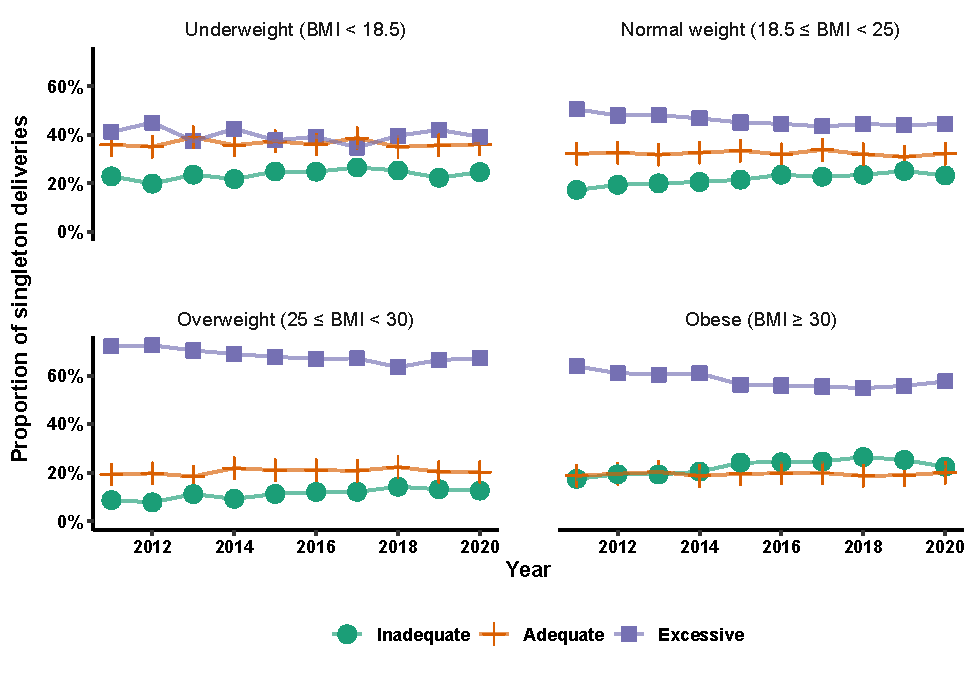
\includegraphics[width=0.95\linewidth,]{03-Determinants_MFIH_files/figure-latex/plot313-1} \end{center}

\begin{table}[H]
\centering
\resizebox{\linewidth}{!}{
\begin{threeparttable}
\begin{tabular}[t]{lllllllllll}
\toprule
\textbf{} & \textbf{2011} & \textbf{2012} & \textbf{2013} & \textbf{2014} & \textbf{2015} & \textbf{2016} & \textbf{2017} & \textbf{2018} & \textbf{2019} & \textbf{2020}\\
\midrule
\cellcolor[HTML]{E1E1E1}{\textbf{Underweight}} & \cellcolor[HTML]{E1E1E1}{\textbf{}} & \cellcolor[HTML]{E1E1E1}{\textbf{}} & \cellcolor[HTML]{E1E1E1}{\textbf{}} & \cellcolor[HTML]{E1E1E1}{\textbf{}} & \cellcolor[HTML]{E1E1E1}{\textbf{}} & \cellcolor[HTML]{E1E1E1}{\textbf{}} & \cellcolor[HTML]{E1E1E1}{\textbf{}} & \cellcolor[HTML]{E1E1E1}{\textbf{}} & \cellcolor[HTML]{E1E1E1}{\textbf{}} & \cellcolor[HTML]{E1E1E1}{\textbf{}}\\
Total deliveries\textsuperscript{a} & 301 & 282 & 246 & 280 & 257 & 250 & 256 & 237 & 269 & 219\\
Inadequate (gain < 12.5 kg) & 22.9$\%$ & 19.9$\%$ & 23.6$\%$ & 21.8$\%$ & 24.9$\%$ & 24.8$\%$ & 26.6$\%$ & 25.3$\%$ & 22.3$\%$ & 24.7$\%$\\
Adequate (12.5 kg $\leq$ gain $\leq$ 18 kg) & 35.9$\%$ & 35.1$\%$ & 39.0$\%$ & 35.7$\%$ & 37.4$\%$ & 36.0$\%$ & 38.7$\%$ & 35.0$\%$ & 35.7$\%$ & 36.1$\%$\\
Excessive (gain > 18 kg) & 41.2$\%$ & 45.0$\%$ & 37.4$\%$ & 42.5$\%$ & 37.7$\%$ & 39.2$\%$ & 34.8$\%$ & 39.7$\%$ & 42.0$\%$ & 39.3$\%$\\
\cellcolor[HTML]{E1E1E1}{\textbf{Normal weight}} & \cellcolor[HTML]{E1E1E1}{\textbf{}} & \cellcolor[HTML]{E1E1E1}{\textbf{}} & \cellcolor[HTML]{E1E1E1}{\textbf{}} & \cellcolor[HTML]{E1E1E1}{\textbf{}} & \cellcolor[HTML]{E1E1E1}{\textbf{}} & \cellcolor[HTML]{E1E1E1}{\textbf{}} & \cellcolor[HTML]{E1E1E1}{\textbf{}} & \cellcolor[HTML]{E1E1E1}{\textbf{}} & \cellcolor[HTML]{E1E1E1}{\textbf{}} & \cellcolor[HTML]{E1E1E1}{\textbf{}}\\
Total deliveries\textsuperscript{a} & 3,038 & 2,995 & 2,934 & 2,873 & 2,625 & 2,609 & 2,619 & 2,493 & 2,413 & 2,450\\
Inadequate (gain < 11.5 kg) & 17.3$\%$ & 19.4$\%$ & 20.0$\%$ & 20.6$\%$ & 21.5$\%$ & 23.5$\%$ & 22.7$\%$ & 23.5$\%$ & 25.1$\%$ & 23.3$\%$\\
Adequate (11.5 kg $\leq$ gain $\leq$ 16 kg) & 32.2$\%$ & 32.7$\%$ & 31.8$\%$ & 32.6$\%$ & 33.4$\%$ & 31.9$\%$ & 33.8$\%$ & 32.0$\%$ & 30.9$\%$ & 32.2$\%$\\
Excessive (gain > 16 kg) & 50.5$\%$ & 47.9$\%$ & 48.1$\%$ & 46.8$\%$ & 45.1$\%$ & 44.5$\%$ & 43.5$\%$ & 44.4$\%$ & 44.0$\%$ & 44.5$\%$\\
\cellcolor[HTML]{E1E1E1}{\textbf{Overweight}} & \cellcolor[HTML]{E1E1E1}{\textbf{}} & \cellcolor[HTML]{E1E1E1}{\textbf{}} & \cellcolor[HTML]{E1E1E1}{\textbf{}} & \cellcolor[HTML]{E1E1E1}{\textbf{}} & \cellcolor[HTML]{E1E1E1}{\textbf{}} & \cellcolor[HTML]{E1E1E1}{\textbf{}} & \cellcolor[HTML]{E1E1E1}{\textbf{}} & \cellcolor[HTML]{E1E1E1}{\textbf{}} & \cellcolor[HTML]{E1E1E1}{\textbf{}} & \cellcolor[HTML]{E1E1E1}{\textbf{}}\\
Total deliveries\textsuperscript{a} & 1,470 & 1,419 & 1,490 & 1,454 & 1,396 & 1,476 & 1,339 & 1,413 & 1,462 & 1,500\\
Inadequate (gain < 7 kg) & 8.7$\%$ & 7.8$\%$ & 11.2$\%$ & 9.2$\%$ & 11.2$\%$ & 12.1$\%$ & 12.1$\%$ & 14.2$\%$ & 13.2$\%$ & 12.6$\%$\\
Adequate (7 kg $\leq$ gain $\leq$ 11.5 kg) & 19.3$\%$ & 19.7$\%$ & 18.5$\%$ & 21.9$\%$ & 21.1$\%$ & 21.0$\%$ & 20.8$\%$ & 22.3$\%$ & 20.4$\%$ & 20.3$\%$\\
Excessive (gain > 11.5 kg) & 72.0$\%$ & 72.4$\%$ & 70.3$\%$ & 68.9$\%$ & 67.7$\%$ & 66.9$\%$ & 67.1$\%$ & 63.5$\%$ & 66.4$\%$ & 67.1$\%$\\
\cellcolor[HTML]{E1E1E1}{\textbf{Obese}} & \cellcolor[HTML]{E1E1E1}{\textbf{}} & \cellcolor[HTML]{E1E1E1}{\textbf{}} & \cellcolor[HTML]{E1E1E1}{\textbf{}} & \cellcolor[HTML]{E1E1E1}{\textbf{}} & \cellcolor[HTML]{E1E1E1}{\textbf{}} & \cellcolor[HTML]{E1E1E1}{\textbf{}} & \cellcolor[HTML]{E1E1E1}{\textbf{}} & \cellcolor[HTML]{E1E1E1}{\textbf{}} & \cellcolor[HTML]{E1E1E1}{\textbf{}} & \cellcolor[HTML]{E1E1E1}{\textbf{}}\\
Total deliveries\textsuperscript{a} & 1,376 & 1,455 & 1,390 & 1,461 & 1,421 & 1,438 & 1,443 & 1,455 & 1,492 & 1,476\\
Inadequate (gain < 5 kg) & 17.4$\%$ & 19.4$\%$ & 19.3$\%$ & 20.4$\%$ & 24.1$\%$ & 24.3$\%$ & 24.6$\%$ & 26.5$\%$ & 25.3$\%$ & 22.4$\%$\\
Adequate (5 kg $\leq$ gain $\leq$ 9 kg) & 18.8$\%$ & 19.6$\%$ & 20.3$\%$ & 18.7$\%$ & 19.6$\%$ & 19.7$\%$ & 19.9$\%$ & 18.7$\%$ & 19.0$\%$ & 20.0$\%$\\
Excessive (gain > 9 kg) & 63.8$\%$ & 61.0$\%$ & 60.4$\%$ & 60.9$\%$ & 56.3$\%$ & 55.9$\%$ & 55.5$\%$ & 54.8$\%$ & 55.8$\%$ & 57.6$\%$\\
\bottomrule
\end{tabular}
\begin{tablenotes}
\item \textit{Note: } 
\item Gestational weight gain according to recommendations made by Health Canada.
\item[a] Number of singleton deliveries in this body mass index category with known pre-pregnancy and delivery weights and height.
\end{tablenotes}
\end{threeparttable}}
\end{table}

\hypertarget{section-314}{%
\section{Missing information about maternal weight and height by year, Nova Scotia, 2011-2020}\label{section-314}}

\begin{table}[H]
\centering
\resizebox{\linewidth}{!}{
\begin{tabular}[t]{lllllllllll}
\toprule
\textbf{} & \textbf{2011} & \textbf{2012} & \textbf{2013} & \textbf{2014} & \textbf{2015} & \textbf{2016} & \textbf{2017} & \textbf{2018} & \textbf{2019} & \textbf{2020}\\
\midrule
Pre-pregnancy weight & 17.4\% & 16.0\% & 15.4\% & 15.7\% & 15.2\% & 14.5\% & 13.1\% & 12.5\% & 13.4\% & 12.3\%\\
Delivery weight & 16.3\% & 17.4\% & 15.8\% & 16.5\% & 17.1\% & 18.3\% & 20.2\% & 18.4\% & 17.5\% & 14.1\%\\
Height & 12.9\% & 11.1\% & 11.2\% & 10.5\% & 7.8\% & 7.9\% & 6.5\% & 5.9\% & 5.9\% & 4.2\%\\
\bottomrule
\end{tabular}}
\end{table}

\hypertarget{section-315}{%
\section{Interpregnancy weight change by year, Nova Scotia, 2011-2020}\label{section-315}}

\begin{center}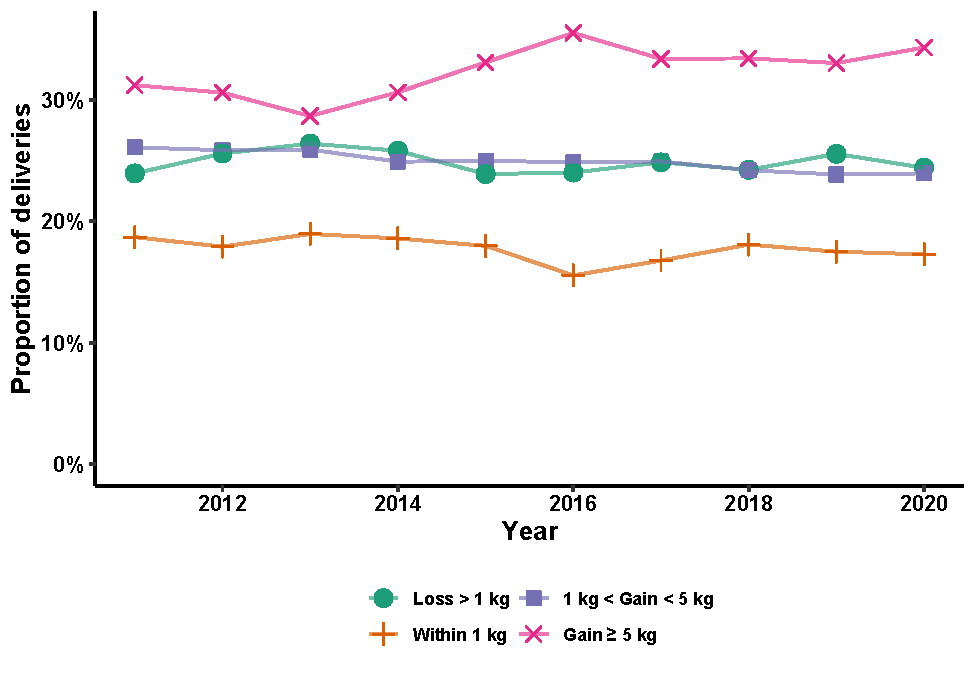
\includegraphics[width=0.9\linewidth,]{03-Determinants_MFIH_files/figure-latex/plot315-1} \end{center}

\begin{table}[H]
\centering
\resizebox{\linewidth}{!}{
\begin{threeparttable}
\begin{tabular}[t]{lllllllllll}
\toprule
\textbf{} & \textbf{2011} & \textbf{2012} & \textbf{2013} & \textbf{2014} & \textbf{2015} & \textbf{2016} & \textbf{2017} & \textbf{2018} & \textbf{2019} & \textbf{2020}\\
\midrule
Total deliveries\textsuperscript{a} & 2,475 & 2,551 & 2,604 & 2,780 & 2,769 & 2,797 & 2,778 & 2,775 & 2,765 & 2,621\\
Loss > 1 kg & 24.0$\%$ & 25.6$\%$ & 26.4$\%$ & 25.8$\%$ & 23.9$\%$ & 24.0$\%$ & 24.9$\%$ & 24.3$\%$ & 25.6$\%$ & 24.4$\%$\\
Within 1 kg & 18.7$\%$ & 17.9$\%$ & 19.0$\%$ & 18.6$\%$ & 18.0$\%$ & 15.6$\%$ & 16.8$\%$ & 18.1$\%$ & 17.5$\%$ & 17.3$\%$\\
1 kg < Gain < 5 kg & 26.1$\%$ & 25.9$\%$ & 25.9$\%$ & 24.9$\%$ & 25.0$\%$ & 24.9$\%$ & 24.9$\%$ & 24.2$\%$ & 23.9$\%$ & 24.0$\%$\\
Gain $\geq$ 5 kg & 31.2$\%$ & 30.6$\%$ & 28.7$\%$ & 30.6$\%$ & 33.1$\%$ & 35.5$\%$ & 33.4$\%$ & 33.4$\%$ & 33.1$\%$ & 34.3$\%$\\
\bottomrule
\end{tabular}
\begin{tablenotes}
\item \textit{Note: } 
\item Interpregnancy weight change is calculated as the pre-pregnancy weight in the index pregnancy minus the pre-pregnancy weight in the woman's preceding pregnancy.
\item[a] With known pre-pregnancy weight in index and preceding pregnancies.
\end{tablenotes}
\end{threeparttable}}
\end{table}

\hypertarget{section-316}{%
\section{Pre-existing diabetes by year, Nova Scotia, 2011-2020}\label{section-316}}

\begin{center}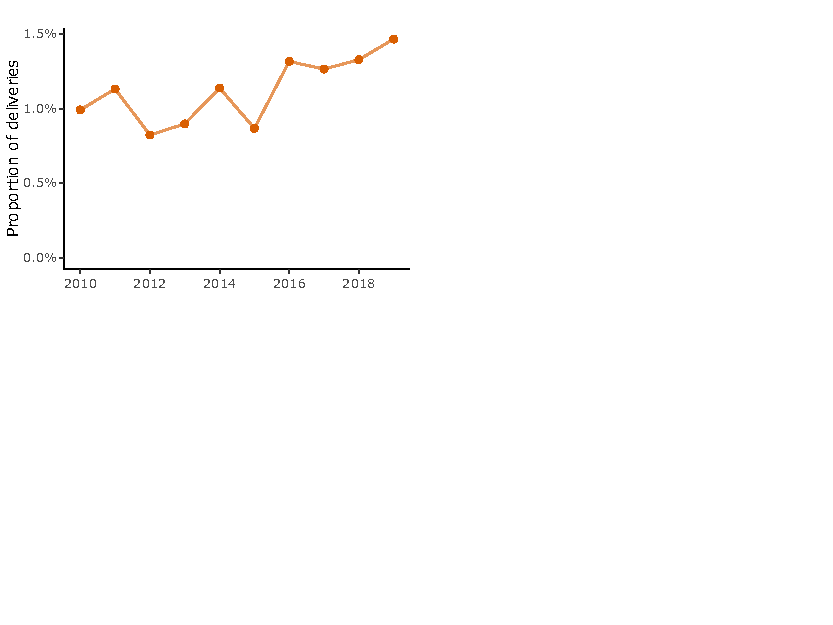
\includegraphics[width=0.9\linewidth,]{03-Determinants_MFIH_files/figure-latex/plot316-1} \end{center}

\begin{table}[H]
\centering
\resizebox{\linewidth}{!}{
\begin{threeparttable}
\begin{tabular}[t]{lllllllllll}
\toprule
\textbf{} & \textbf{2011} & \textbf{2012} & \textbf{2013} & \textbf{2014} & \textbf{2015} & \textbf{2016} & \textbf{2017} & \textbf{2018} & \textbf{2019} & \textbf{2020}\\
\midrule
Total deliveries & 8,766 & 8,621 & 8,329 & 8,516 & 8,053 & 8,197 & 8,115 & 7,839 & 7,943 & 7,494\\
Pre-existing diabetes & 1.07$\%$ & 0.79$\%$ & 0.85$\%$ & 1.08$\%$ & 0.84$\%$ & 1.34$\%$ & 1.24$\%$ & 1.31$\%$ & 1.42$\%$ & 1.33$\%$\\
\bottomrule
\end{tabular}
\begin{tablenotes}
\item \textit{Note: } 
\item Maternal history of either Type 1 or Type 2 diabetes mellitus prior to the current pregnancy.
\end{tablenotes}
\end{threeparttable}}
\end{table}

\hypertarget{section-317}{%
\section{Pre-existing hypertension by year, Nova Scotia, 2011-2020}\label{section-317}}

\begin{center}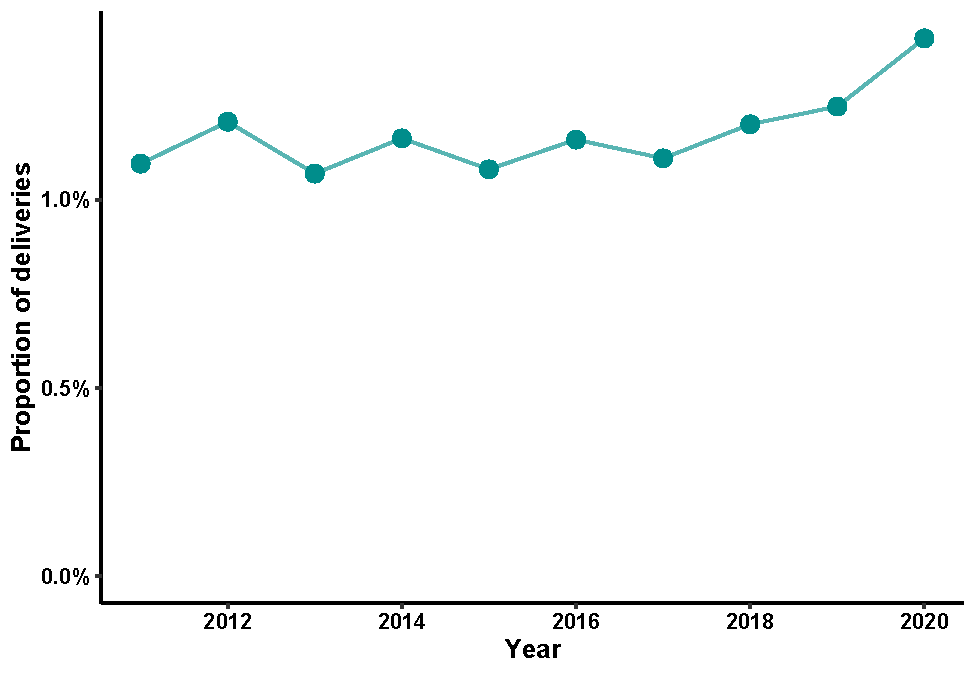
\includegraphics[width=0.9\linewidth,]{03-Determinants_MFIH_files/figure-latex/plot317-1} \end{center}

\begin{table}[H]
\centering
\resizebox{\linewidth}{!}{
\begin{threeparttable}
\begin{tabular}[t]{lllllllllll}
\toprule
\textbf{} & \textbf{2011} & \textbf{2012} & \textbf{2013} & \textbf{2014} & \textbf{2015} & \textbf{2016} & \textbf{2017} & \textbf{2018} & \textbf{2019} & \textbf{2020}\\
\midrule
Total deliveries & 8,764 & 8,618 & 8,325 & 8,514 & 8,051 & 8,194 & 8,111 & 7,832 & 7,938 & 7,491\\
Pre-existing hypertension & 1.10$\%$ & 1.21$\%$ & 1.07$\%$ & 1.16$\%$ & 1.07$\%$ & 1.16$\%$ & 1.11$\%$ & 1.20$\%$ & 1.25$\%$ & 1.43$\%$\\
\bottomrule
\end{tabular}
\begin{tablenotes}
\item \textit{Note: } 
\item Maternal history of hypertensive disease prior to the current pregnancy or prior to 20 weeks gestation in the current pregnancy.
\end{tablenotes}
\end{threeparttable}}
\end{table}

\hypertarget{section-318}{%
\section{Number of pre-pregnancy risk factors by year, Nova Scotia, 2011-2020}\label{section-318}}

\begin{center}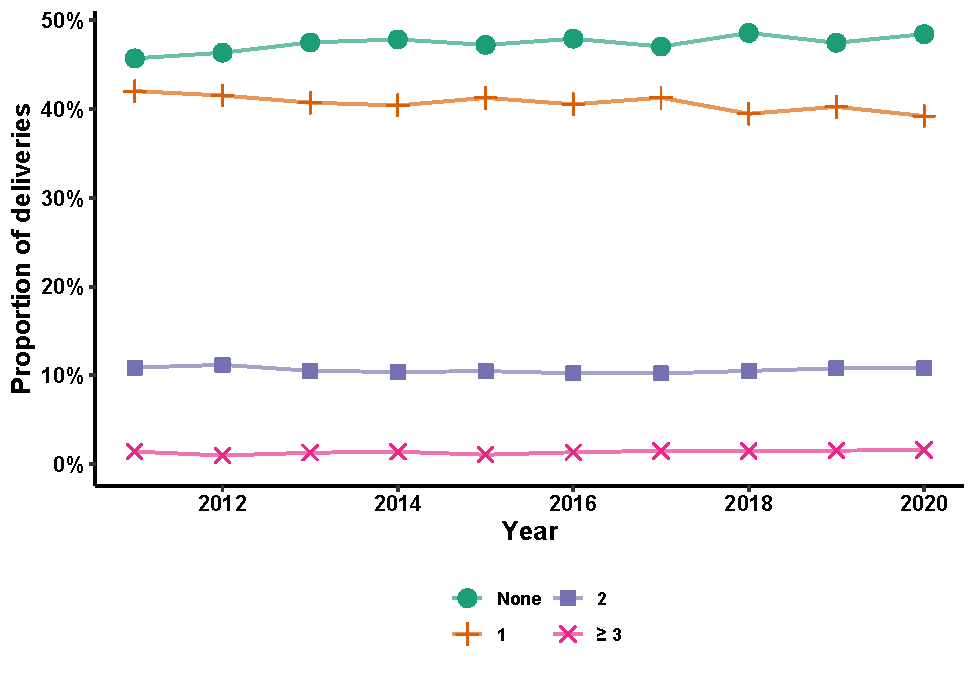
\includegraphics[width=0.9\linewidth,]{03-Determinants_MFIH_files/figure-latex/plot318-1} \end{center}

\begin{table}[H]
\centering
\resizebox{\linewidth}{!}{
\begin{threeparttable}
\begin{tabular}[t]{lllllllllll}
\toprule
\textbf{} & \textbf{2011} & \textbf{2012} & \textbf{2013} & \textbf{2014} & \textbf{2015} & \textbf{2016} & \textbf{2017} & \textbf{2018} & \textbf{2019} & \textbf{2020}\\
\midrule
Total deliveries\textsuperscript{a} & 6,858 & 6,883 & 6,690 & 6,800 & 6,505 & 6,644 & 6,765 & 6,624 & 6,626 & 6,431\\
None & 45.7$\%$ & 46.3$\%$ & 47.5$\%$ & 47.9$\%$ & 47.2$\%$ & 47.9$\%$ & 47.1$\%$ & 48.6$\%$ & 47.5$\%$ & 48.5$\%$\\
1 & 42.0$\%$ & 41.5$\%$ & 40.7$\%$ & 40.4$\%$ & 41.3$\%$ & 40.5$\%$ & 41.3$\%$ & 39.5$\%$ & 40.3$\%$ & 39.2$\%$\\
2 & 10.9$\%$ & 11.2$\%$ & 10.5$\%$ & 10.4$\%$ & 10.5$\%$ & 10.2$\%$ & 10.2$\%$ & 10.5$\%$ & 10.8$\%$ & 10.8$\%$\\
$\geq$ 3 & 1.4$\%$ & 1.0$\%$ & 1.2$\%$ & 1.4$\%$ & 1.0$\%$ & 1.3$\%$ & 1.5$\%$ & 1.5$\%$ & 1.5$\%$ & 1.5$\%$\\
\bottomrule
\end{tabular}
\begin{tablenotes}
\item \textit{Note: } 
\item Pre-pregnancy risk factors included maternal age $\geq$ 35 years, BMI $\geq$ 30 kg/$m^{2}$ , smoking, pre-existing diabetes, and pre-existing hypertension.
\end{tablenotes}
\end{threeparttable}}
\end{table}

\hypertarget{section-319}{%
\section{Use of medication for depression or anxiety during pregnancy by year, Nova Scotia, 2011-2020}\label{section-319}}

\begin{center}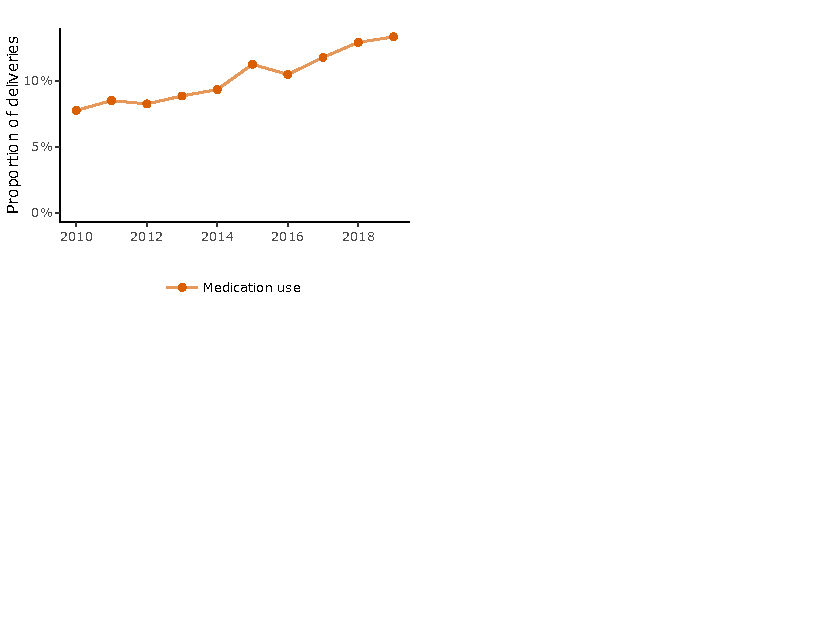
\includegraphics[width=0.9\linewidth,]{03-Determinants_MFIH_files/figure-latex/plot319-1} \end{center}

\begin{table}[H]
\centering
\resizebox{\linewidth}{!}{
\begin{threeparttable}
\begin{tabular}[t]{lllllllllll}
\toprule
\textbf{} & \textbf{2011} & \textbf{2012} & \textbf{2013} & \textbf{2014} & \textbf{2015} & \textbf{2016} & \textbf{2017} & \textbf{2018} & \textbf{2019} & \textbf{2020}\\
\midrule
Total deliveries & 8,764 & 8,618 & 8,325 & 8,514 & 8,051 & 8,194 & 8,111 & 7,832 & 7,938 & 7,491\\
Medication use & 8.4$\%$ & 8.3$\%$ & 8.8$\%$ & 9.2$\%$ & 11.3$\%$ & 10.4$\%$ & 11.7$\%$ & 12.9$\%$ & 13.2$\%$ & 12.8$\%$\\
\bottomrule
\end{tabular}
\begin{tablenotes}
\item \textit{Note: } 
\item If recorded on the Nova Scotia Prenatal Record.
\end{tablenotes}
\end{threeparttable}}
\end{table}

\hypertarget{section-320}{%
\section{Breastfeeding status during hospital stay by year, Nova Scotia, 2011-2020}\label{section-320}}

\begin{center}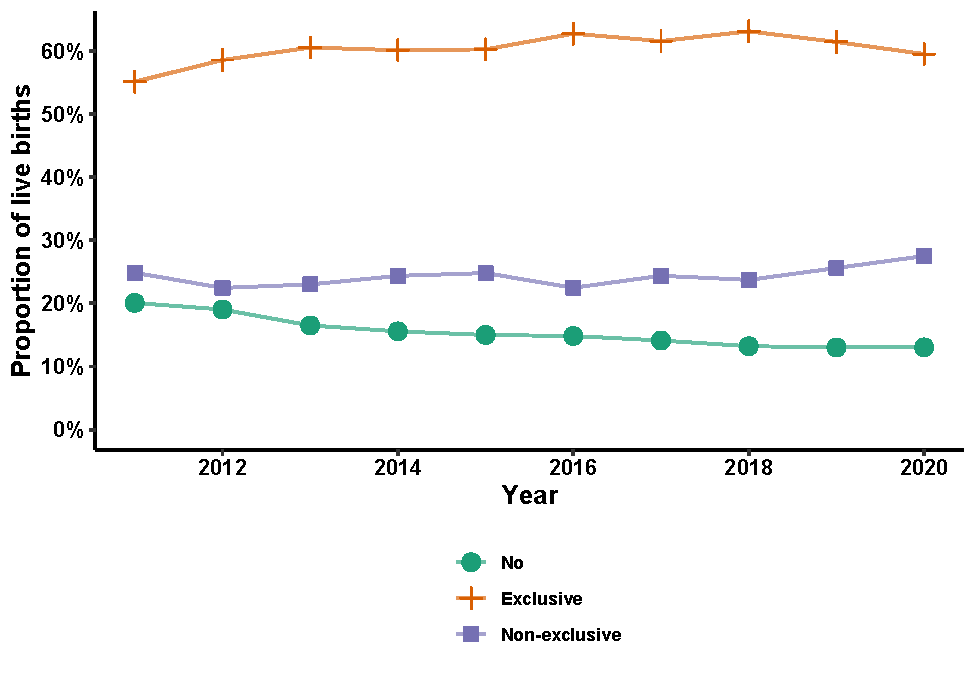
\includegraphics[width=0.9\linewidth,]{03-Determinants_MFIH_files/figure-latex/plot320-1} \end{center}

\begin{table}[H]
\centering
\resizebox{\linewidth}{!}{
\begin{threeparttable}
\begin{tabular}[t]{lllllllllll}
\toprule
\textbf{} & \textbf{2011} & \textbf{2012} & \textbf{2013} & \textbf{2014} & \textbf{2015} & \textbf{2016} & \textbf{2017} & \textbf{2018} & \textbf{2019} & \textbf{2020}\\
\midrule
Total deliveries\textsuperscript{a} & 8,849 & 8,704 & 8,423 & 8,592 & 8,119 & 8,271 & 8,199 & 7,903 & 8,024 & 7,551\\
Exclusive & 54.9$\%$ & 58.3$\%$ & 60.3$\%$ & 59.9$\%$ & 60.1$\%$ & 62.5$\%$ & 61.3$\%$ & 62.8$\%$ & 61.1$\%$ & 59.2$\%$\\
Non-exclusive & 24.7$\%$ & 22.4$\%$ & 22.9$\%$ & 24.3$\%$ & 24.7$\%$ & 22.4$\%$ & 24.3$\%$ & 23.6$\%$ & 25.5$\%$ & 27.3$\%$\\
\bottomrule
\end{tabular}
\begin{tablenotes}
\item \textit{Note: } 
\item Describes the method of infant feeding during the hospital stay. Breastfeeding refers to when the infant was given breast milk: Exclusive denotes that the infant received only breast milk and non-exclusive denotes that the infant received breast milk with supplementation.
\item[a] With known breastfeeding status.
\end{tablenotes}
\end{threeparttable}}
\end{table}

\hypertarget{section-4}{%
\chapter{Labour and Birth Processes}\label{section-4}}

\hypertarget{section-41}{%
\section{Labour induction by parity and year, Nova Scotia, 2011-2020}\label{section-41}}

\begin{center}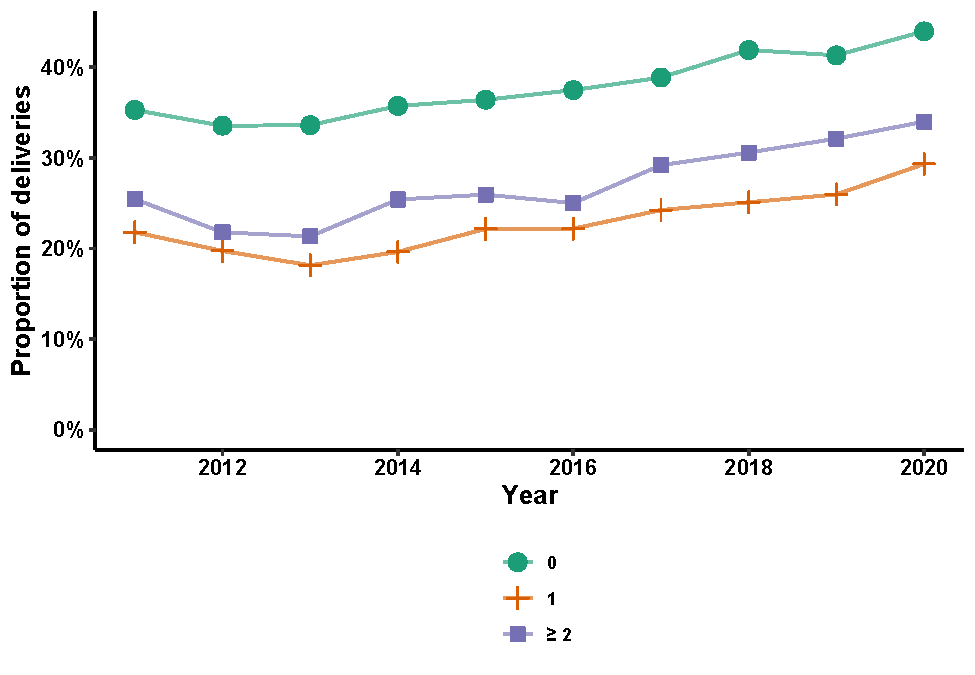
\includegraphics[width=0.9\linewidth,]{04-Labour_Birth_Process_files/figure-latex/plot41-1} \end{center}

\begin{table}[H]
\centering
\resizebox{\linewidth}{!}{
\begin{threeparttable}
\begin{tabular}[t]{lllllllllll}
\toprule
\textbf{Parity} & \textbf{2011} & \textbf{2012} & \textbf{2013} & \textbf{2014} & \textbf{2015} & \textbf{2016} & \textbf{2017} & \textbf{2018} & \textbf{2019} & \textbf{2020}\\
\midrule
\cellcolor[HTML]{E1E1E1}{\textbf{0}} & \cellcolor[HTML]{E1E1E1}{\textbf{}} & \cellcolor[HTML]{E1E1E1}{\textbf{}} & \cellcolor[HTML]{E1E1E1}{\textbf{}} & \cellcolor[HTML]{E1E1E1}{\textbf{}} & \cellcolor[HTML]{E1E1E1}{\textbf{}} & \cellcolor[HTML]{E1E1E1}{\textbf{}} & \cellcolor[HTML]{E1E1E1}{\textbf{}} & \cellcolor[HTML]{E1E1E1}{\textbf{}} & \cellcolor[HTML]{E1E1E1}{\textbf{}} & \cellcolor[HTML]{E1E1E1}{\textbf{}}\\
Total deliveries & 4,093 & 4,110 & 3,880 & 3,878 & 3,618 & 3,672 & 3,632 & 3,370 & 3,550 & 3,303\\
Induction attempted ($\%$) & 35.2$\%$ & 33.6$\%$ & 33.7$\%$ & 35.7$\%$ & 36.2$\%$ & 37.6$\%$ & 38.8$\%$ & 41.9$\%$ & 41.2$\%$ & 43.8$\%$\\
\cellcolor[HTML]{E1E1E1}{\textbf{1}} & \cellcolor[HTML]{E1E1E1}{\textbf{}} & \cellcolor[HTML]{E1E1E1}{\textbf{}} & \cellcolor[HTML]{E1E1E1}{\textbf{}} & \cellcolor[HTML]{E1E1E1}{\textbf{}} & \cellcolor[HTML]{E1E1E1}{\textbf{}} & \cellcolor[HTML]{E1E1E1}{\textbf{}} & \cellcolor[HTML]{E1E1E1}{\textbf{}} & \cellcolor[HTML]{E1E1E1}{\textbf{}} & \cellcolor[HTML]{E1E1E1}{\textbf{}} & \cellcolor[HTML]{E1E1E1}{\textbf{}}\\
Total deliveries & 3,039 & 3,058 & 3,000 & 3,109 & 2,951 & 2,926 & 2,812 & 2,804 & 2,840 & 2,687\\
Induction attempted ($\%$) & 21.8$\%$ & 19.7$\%$ & 18.4$\%$ & 19.6$\%$ & 22.1$\%$ & 22.4$\%$ & 24.1$\%$ & 25.1$\%$ & 26.2$\%$ & 29.3$\%$\\
\cellcolor[HTML]{E1E1E1}{\textbf{$\geq$ 2}} & \cellcolor[HTML]{E1E1E1}{\textbf{}} & \cellcolor[HTML]{E1E1E1}{\textbf{}} & \cellcolor[HTML]{E1E1E1}{\textbf{}} & \cellcolor[HTML]{E1E1E1}{\textbf{}} & \cellcolor[HTML]{E1E1E1}{\textbf{}} & \cellcolor[HTML]{E1E1E1}{\textbf{}} & \cellcolor[HTML]{E1E1E1}{\textbf{}} & \cellcolor[HTML]{E1E1E1}{\textbf{}} & \cellcolor[HTML]{E1E1E1}{\textbf{}} & \cellcolor[HTML]{E1E1E1}{\textbf{}}\\
Total deliveries & 1,772 & 1,597 & 1,586 & 1,677 & 1,606 & 1,720 & 1,807 & 1,776 & 1,690 & 1,614\\
Induction attempted ($\%$) & 25.5$\%$ & 21.6$\%$ & 21.2$\%$ & 25.6$\%$ & 26.1$\%$ & 25.1$\%$ & 29.2$\%$ & 30.8$\%$ & 32.1$\%$ & 34.0$\%$\\
\bottomrule
\end{tabular}
\begin{tablenotes}
\item \textit{Note: } 
\item The initiation of contractions in a pregnant woman who is not in labour to help her achieve a vaginal birth within 24 to 48 hours.
\end{tablenotes}
\end{threeparttable}}
\end{table}

\hypertarget{section-42}{%
\section{Indication for labour induction by year, Nova Scotia, 2011-2020}\label{section-42}}

\begin{center}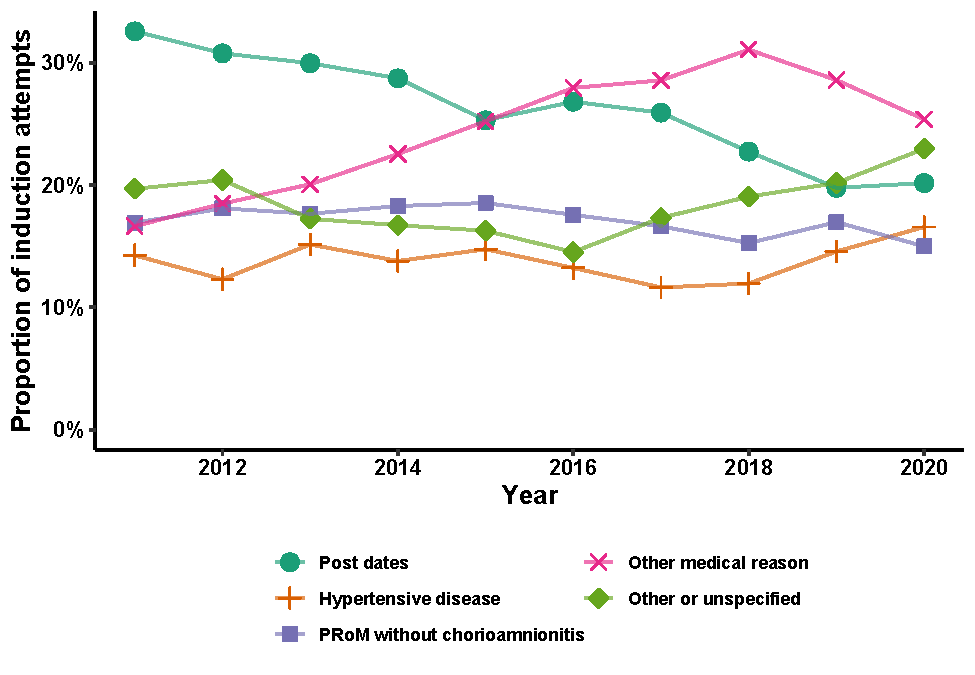
\includegraphics[width=0.9\linewidth,]{04-Labour_Birth_Process_files/figure-latex/plot42-1} \end{center}

\begin{table}[H]
\centering
\resizebox{\linewidth}{!}{
\begin{tabular}[t]{lllllllllll}
\toprule
\textbf{} & \textbf{2011} & \textbf{2012} & \textbf{2013} & \textbf{2014} & \textbf{2015} & \textbf{2016} & \textbf{2017} & \textbf{2018} & \textbf{2019} & \textbf{2020}\\
\midrule
Total induction attempts & 2,556 & 2,328 & 2,194 & 2,424 & 2,381 & 2,467 & 2,617 & 2,663 & 2,748 & 2,784\\
Post dates & 32.6$\%$ & 30.8$\%$ & 29.9$\%$ & 28.7$\%$ & 25.3$\%$ & 26.8$\%$ & 25.9$\%$ & 22.7$\%$ & 19.8$\%$ & 20.2$\%$\\
Hypertensive disease & 14.2$\%$ & 12.3$\%$ & 15.1$\%$ & 13.8$\%$ & 14.7$\%$ & 13.2$\%$ & 11.6$\%$ & 11.9$\%$ & 14.6$\%$ & 16.6$\%$\\
PRoM\textsuperscript{a} without chorioamnionitis & 16.9$\%$ & 18.1$\%$ & 17.6$\%$ & 18.3$\%$ & 18.5$\%$ & 17.6$\%$ & 16.6$\%$ & 15.2$\%$ & 17.0$\%$ & 15.0$\%$\\
Other medical reason\textsuperscript{b} & 16.6$\%$ & 18.5$\%$ & 20.1$\%$ & 22.5$\%$ & 25.2$\%$ & 27.9$\%$ & 28.5$\%$ & 31.1$\%$ & 28.6$\%$ & 25.4$\%$\\
Other or unspecified & 19.7$\%$ & 20.4$\%$ & 17.2$\%$ & 16.7$\%$ & 16.3$\%$ & 14.5$\%$ & 17.3$\%$ & 19.0$\%$ & 20.2$\%$ & 23.0$\%$\\
\bottomrule
\multicolumn{11}{l}{\rule{0pt}{1em}\textsuperscript{a} PRoM: Prelabour rupture of membranes.}\\
\multicolumn{11}{l}{\rule{0pt}{1em}\textsuperscript{b} Please see Glossary under 'Indication for labour induction' for complete list.}\\
\end{tabular}}
\end{table}

\hypertarget{section-43}{%
\section{Medical augmentation of labour among women with spontaneous onset of labour by year, Nova Scotia, 2011-2020}\label{section-43}}

\begin{center}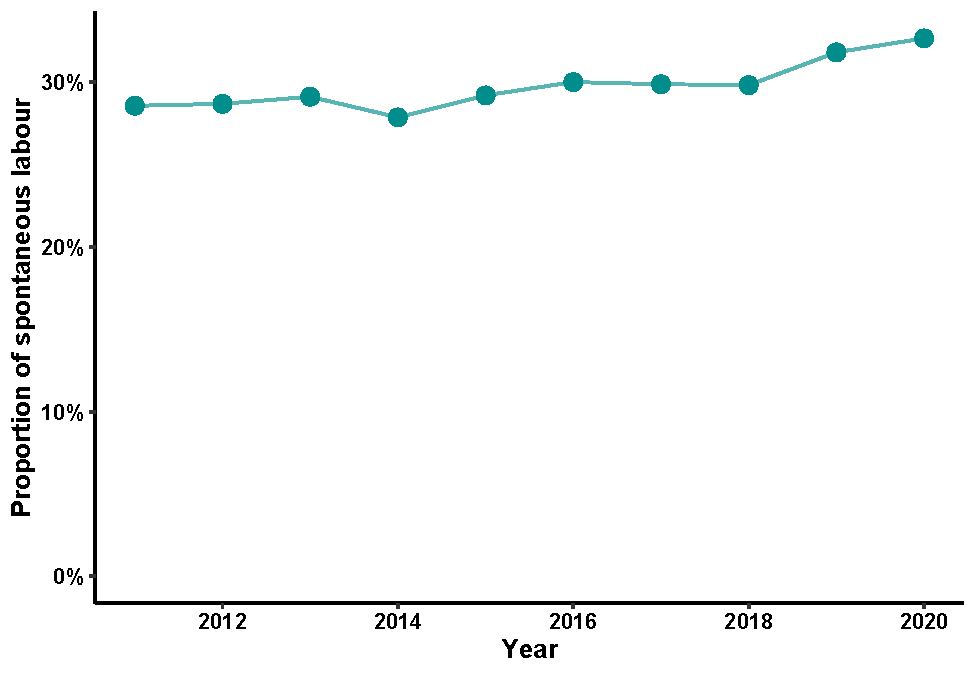
\includegraphics[width=0.9\linewidth,]{04-Labour_Birth_Process_files/figure-latex/plot43-1} \end{center}

\begin{table}[H]
\centering
\resizebox{\linewidth}{!}{
\begin{threeparttable}
\begin{tabular}[t]{lllllllllll}
\toprule
\textbf{} & \textbf{2011} & \textbf{2012} & \textbf{2013} & \textbf{2014} & \textbf{2015} & \textbf{2016} & \textbf{2017} & \textbf{2018} & \textbf{2019} & \textbf{2020}\\
\midrule
Total spontaneous labour & 5,119 & 5,209 & 4,995 & 4,975 & 4,686 & 4,650 & 4,416 & 4,136 & 4,141 & 3,623\\
Augmented & 28.6\% & 28.7\% & 29.1\% & 27.9\% & 29.2\% & 30.0\% & 29.9\% & 29.8\% & 31.8\% & 32.7\%\\
\bottomrule
\end{tabular}
\begin{tablenotes}
\item \textit{Note: } 
\item Use of oxytocin to improve contractions after labour has started spontaneously.
\end{tablenotes}
\end{threeparttable}}
\end{table}

\hypertarget{section-44}{%
\section{Use of regional anesthesia with vaginal delivery by year, Nova Scotia, 2011-2020}\label{section-44}}

\begin{center}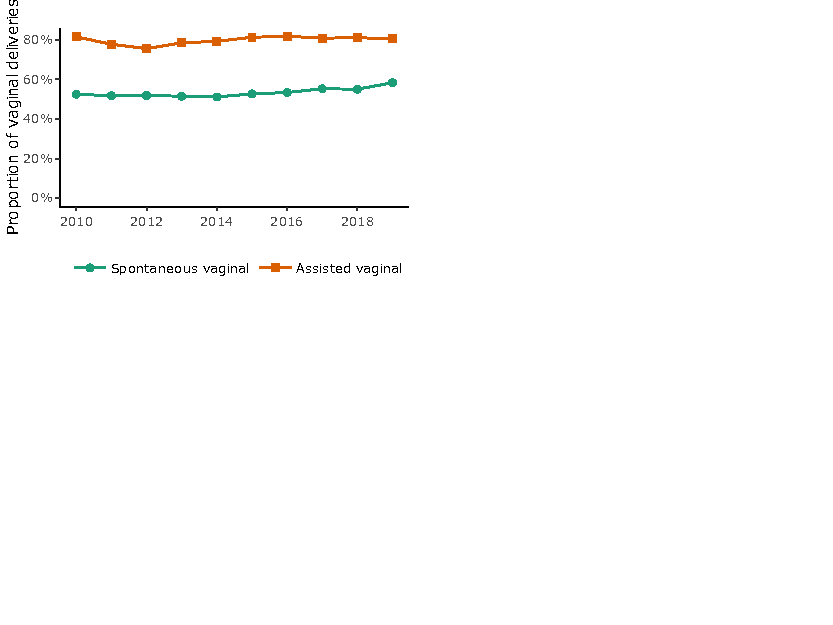
\includegraphics[width=0.9\linewidth,]{04-Labour_Birth_Process_files/figure-latex/plot44-1} \end{center}

\begin{table}[H]
\centering
\resizebox{\linewidth}{!}{
\begin{threeparttable}
\begin{tabular}[t]{lllllllllll}
\toprule
\textbf{Type of delivery} & \textbf{2011} & \textbf{2012} & \textbf{2013} & \textbf{2014} & \textbf{2015} & \textbf{2016} & \textbf{2017} & \textbf{2018} & \textbf{2019} & \textbf{2020}\\
\midrule
\cellcolor[HTML]{E1E1E1}{\textbf{Spontaneous}} & \cellcolor[HTML]{E1E1E1}{\textbf{}} & \cellcolor[HTML]{E1E1E1}{\textbf{}} & \cellcolor[HTML]{E1E1E1}{\textbf{}} & \cellcolor[HTML]{E1E1E1}{\textbf{}} & \cellcolor[HTML]{E1E1E1}{\textbf{}} & \cellcolor[HTML]{E1E1E1}{\textbf{}} & \cellcolor[HTML]{E1E1E1}{\textbf{}} & \cellcolor[HTML]{E1E1E1}{\textbf{}} & \cellcolor[HTML]{E1E1E1}{\textbf{}} & \cellcolor[HTML]{E1E1E1}{\textbf{}}\\
Total deliveries & 5,648 & 5,667 & 5,433 & 5,591 & 5,315 & 5,293 & 5,210 & 4,924 & 4,859 & 4,517\\
Anesthesia ($\%$)\textsuperscript{a} & 51.4$\%$ & 51.8$\%$ & 51.4$\%$ & 51.2$\%$ & 52.4$\%$ & 53.1$\%$ & 55.2$\%$ & 54.9$\%$ & 58.4$\%$ & 59.1$\%$\\
\cellcolor[HTML]{E1E1E1}{\textbf{Assisted}} & \cellcolor[HTML]{E1E1E1}{\textbf{}} & \cellcolor[HTML]{E1E1E1}{\textbf{}} & \cellcolor[HTML]{E1E1E1}{\textbf{}} & \cellcolor[HTML]{E1E1E1}{\textbf{}} & \cellcolor[HTML]{E1E1E1}{\textbf{}} & \cellcolor[HTML]{E1E1E1}{\textbf{}} & \cellcolor[HTML]{E1E1E1}{\textbf{}} & \cellcolor[HTML]{E1E1E1}{\textbf{}} & \cellcolor[HTML]{E1E1E1}{\textbf{}} & \cellcolor[HTML]{E1E1E1}{\textbf{}}\\
Total deliveries & 761 & 711 & 642 & 661 & 639 & 690 & 743 & 732 & 775 & 701\\
Anesthesia ($\%$)\textsuperscript{a} & 77.8$\%$ & 75.4$\%$ & 78.5$\%$ & 78.8$\%$ & 81.5$\%$ & 81.3$\%$ & 81.3$\%$ & 80.5$\%$ & 80.4$\%$ & 85.4$\%$\\
\bottomrule
\end{tabular}
\begin{tablenotes}
\item[a] Regional anesthesia including epidural, spinal, and/or pudendal anesthesia during labour and/or delivery.
\end{tablenotes}
\end{threeparttable}}
\end{table}

\hypertarget{section-45}{%
\section{Type of delivery by year, Nova Scotia, 2011-2020}\label{section-45}}

\begin{center}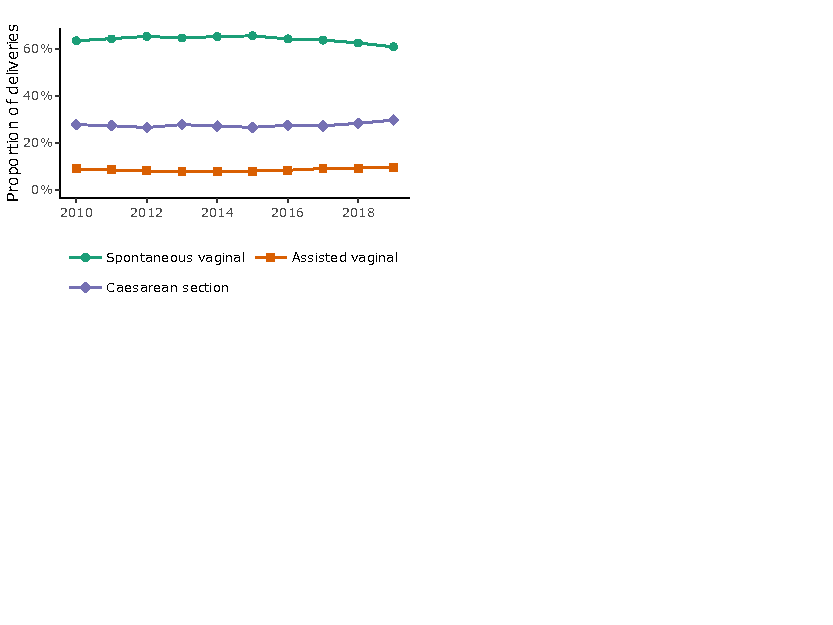
\includegraphics[width=0.9\linewidth,]{04-Labour_Birth_Process_files/figure-latex/plot45-1} \end{center}

\begin{table}[H]
\centering
\resizebox{\linewidth}{!}{
\begin{threeparttable}
\begin{tabular}[t]{lllllllllll}
\toprule
\textbf{} & \textbf{2011} & \textbf{2012} & \textbf{2013} & \textbf{2014} & \textbf{2015} & \textbf{2016} & \textbf{2017} & \textbf{2018} & \textbf{2019} & \textbf{2020}\\
\midrule
Total deliveries\textsuperscript{a} & 8,763 & 8,618 & 8,325 & 8,513 & 8,051 & 8,193 & 8,110 & 7,831 & 7,938 & 7,491\\
Spontaneous vaginal & 64.5$\%$ & 65.8$\%$ & 65.3$\%$ & 65.7$\%$ & 66.0$\%$ & 64.6$\%$ & 64.2$\%$ & 62.9$\%$ & 61.2$\%$ & 60.3$\%$\\
Assisted vaginal & 8.7$\%$ & 8.3$\%$ & 7.7$\%$ & 7.8$\%$ & 7.9$\%$ & 8.4$\%$ & 9.2$\%$ & 9.3$\%$ & 9.8$\%$ & 9.4$\%$\\
Caesarean section & 26.9$\%$ & 26.0$\%$ & 27.0$\%$ & 26.6$\%$ & 26.0$\%$ & 27.0$\%$ & 26.6$\%$ & 27.8$\%$ & 29.0$\%$ & 30.3$\%$\\
\bottomrule
\end{tabular}
\begin{tablenotes}
\item[a] With known type of delivery.
\end{tablenotes}
\end{threeparttable}}
\end{table}

\hypertarget{section-46}{%
\section{Stage of labour before Caesarean delivery by year, Nova Scotia, 2011-2020}\label{section-46}}

\begin{center}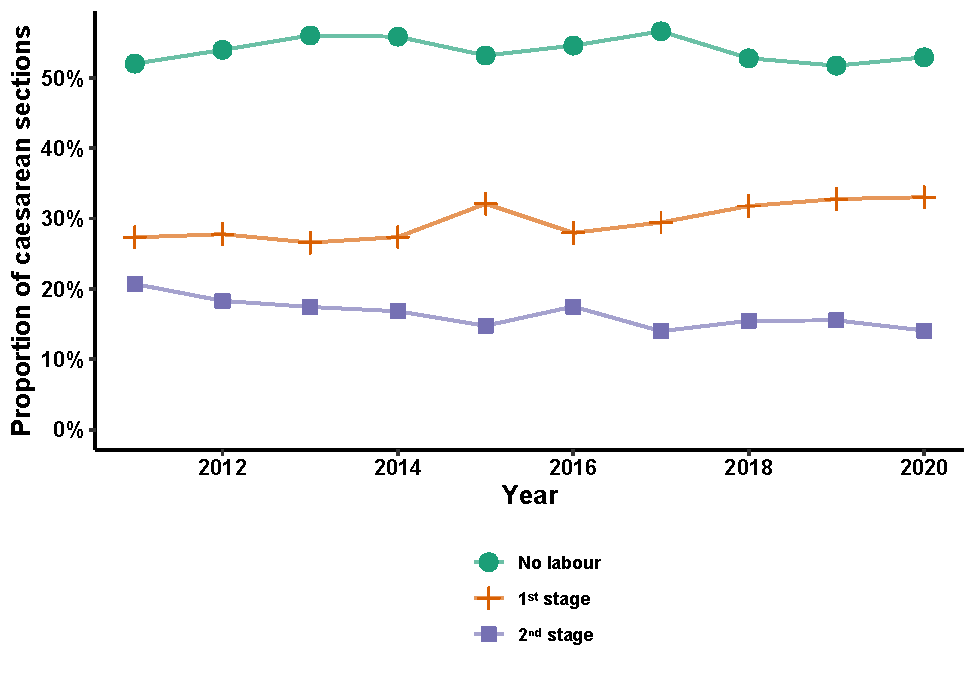
\includegraphics[width=0.9\linewidth,]{04-Labour_Birth_Process_files/figure-latex/plot46-1} \end{center}

\begin{table}[H]
\centering
\resizebox{\linewidth}{!}{
\begin{threeparttable}
\begin{tabular}[t]{lllllllllll}
\toprule
\textbf{} & \textbf{2011} & \textbf{2012} & \textbf{2013} & \textbf{2014} & \textbf{2015} & \textbf{2016} & \textbf{2017} & \textbf{2018} & \textbf{2019} & \textbf{2020}\\
\midrule
Total caesarean sections & 2,431 & 2,323 & 2,341 & 2,343 & 2,175 & 2,282 & 2,239 & 2,244 & 2,396 & 2,344\\
No labour & 52.0$\%$ & 53.9$\%$ & 56.0$\%$ & 55.8$\%$ & 53.1$\%$ & 54.6$\%$ & 56.6$\%$ & 52.8$\%$ & 51.7$\%$ & 52.9$\%$\\
$1^{st}$ stage & 27.3$\%$ & 27.8$\%$ & 26.6$\%$ & 27.4$\%$ & 32.1$\%$ & 28.0$\%$ & 29.4$\%$ & 31.8$\%$ & 32.8$\%$ & 33.0$\%$\\
$2^{nd}$ stage & 20.7$\%$ & 18.3$\%$ & 17.4$\%$ & 16.8$\%$ & 14.8$\%$ & 17.5$\%$ & 14.0$\%$ & 15.5$\%$ & 15.5$\%$ & 14.1$\%$\\
\bottomrule
\end{tabular}
\begin{tablenotes}
\item \textit{Note: } 
\item The $1^{st}$ stage is the period from the onset of labour until the cervix is fully dilated (10 cm). The $2^{nd}$ stage is the period from 10 cm dilation of the cervix until the baby is delivered.
\end{tablenotes}
\end{threeparttable}}
\end{table}

\hypertarget{section-47}{%
\section{Primary indication for Caesarean delivery by year, Nova Scotia, 2011-2020}\label{section-47}}

\begin{center}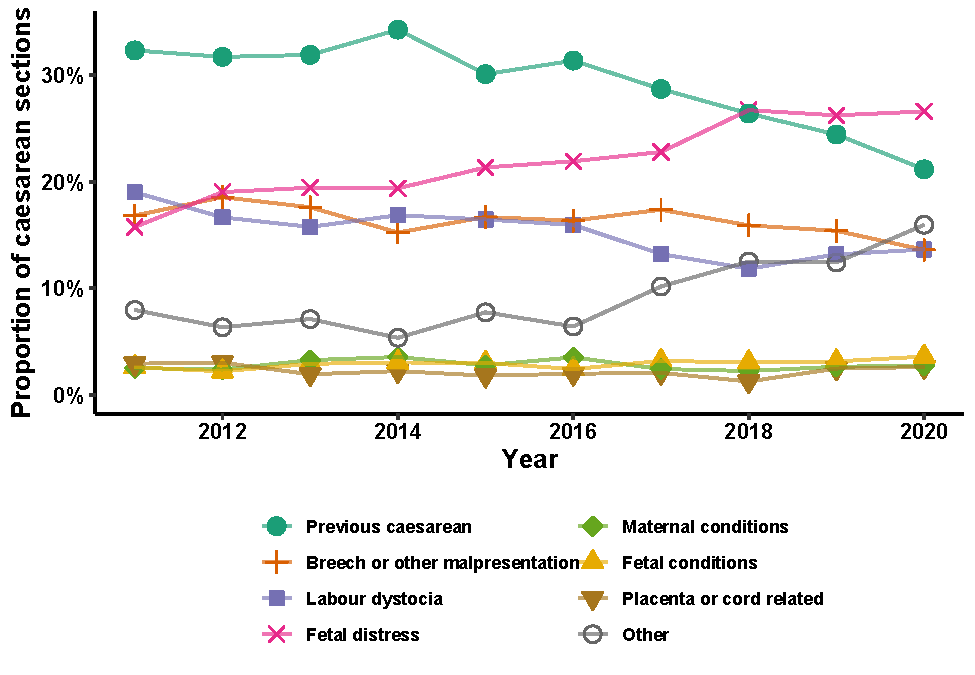
\includegraphics[width=0.9\linewidth,]{04-Labour_Birth_Process_files/figure-latex/plot47-1} \end{center}

\begin{table}[H]
\centering
\resizebox{\linewidth}{!}{
\begin{tabular}[t]{lllllllllll}
\toprule
\textbf{} & \textbf{2011} & \textbf{2012} & \textbf{2013} & \textbf{2014} & \textbf{2015} & \textbf{2016} & \textbf{2017} & \textbf{2018} & \textbf{2019} & \textbf{2020}\\
\midrule
Total caesarean sections & 2,431 & 2,323 & 2,341 & 2,343 & 2,175 & 2,282 & 2,239 & 2,244 & 2,396 & 2,344\\
Previous caesarean & 32.3$\%$ & 31.7$\%$ & 31.9$\%$ & 34.2$\%$ & 30.1$\%$ & 31.3$\%$ & 28.7$\%$ & 26.4$\%$ & 24.4$\%$ & 21.2$\%$\\
Breech or other malpresentation & 16.8$\%$ & 18.6$\%$ & 17.6$\%$ & 15.2$\%$ & 16.7$\%$ & 16.3$\%$ & 17.4$\%$ & 15.9$\%$ & 15.4$\%$ & 13.6$\%$\\
Labour dystocia & 19.0$\%$ & 16.7$\%$ & 15.8$\%$ & 16.9$\%$ & 16.5$\%$ & 16.0$\%$ & 13.2$\%$ & 11.9$\%$ & 13.2$\%$ & 13.7$\%$\\
Fetal distress & 15.8$\%$ & 19.0$\%$ & 19.4$\%$ & 19.4$\%$ & 21.3$\%$ & 21.9$\%$ & 22.8$\%$ & 26.7$\%$ & 26.2$\%$ & 26.6$\%$\\
Maternal conditions & 2.6$\%$ & 2.4$\%$ & 3.3$\%$ & 3.6$\%$ & 2.8$\%$ & 3.5$\%$ & 2.5$\%$ & 2.3$\%$ & 2.7$\%$ & 2.8$\%$\\
Fetal conditions & 2.6$\%$ & 2.2$\%$ & 2.9$\%$ & 3.1$\%$ & 3.0$\%$ & 2.5$\%$ & 3.2$\%$ & 3.1$\%$ & 3.2$\%$ & 3.6$\%$\\
Placenta or cord related & 3.0$\%$ & 3.1$\%$ & 2.0$\%$ & 2.3$\%$ & 1.8$\%$ & 2.0$\%$ & 2.1$\%$ & 1.3$\%$ & 2.5$\%$ & 2.6$\%$\\
Other & 8.0$\%$ & 6.4$\%$ & 7.1$\%$ & 5.4$\%$ & 7.8$\%$ & 6.4$\%$ & 10.2$\%$ & 12.5$\%$ & 12.4$\%$ & 16.0$\%$\\
\bottomrule
\end{tabular}}
\end{table}

\hypertarget{section-48}{%
\section{Caesarean delivery by Robson group and year, Nova Scotia, 2011-2020}\label{section-48}}

\begin{center}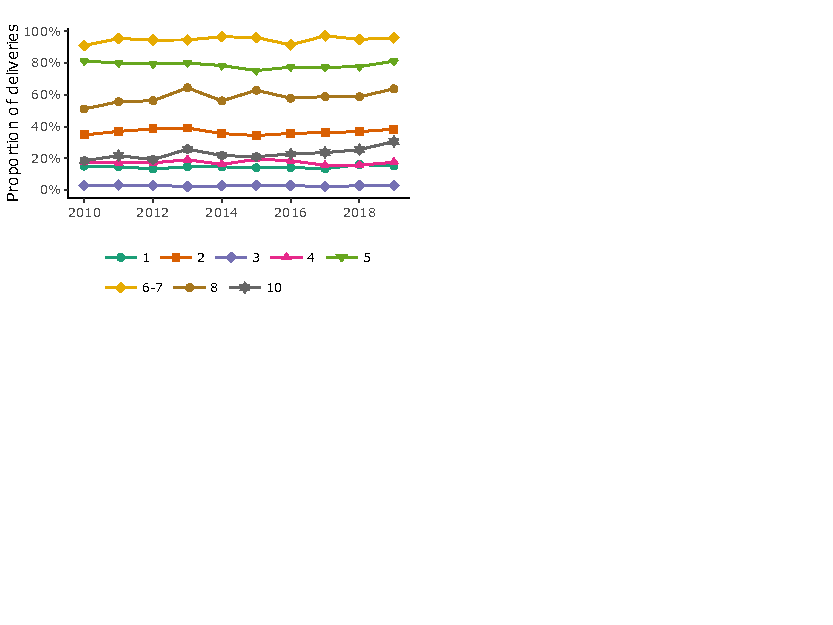
\includegraphics[width=0.9\linewidth,]{04-Labour_Birth_Process_files/figure-latex/plot48-1} \end{center}

\begin{table}[H]
\centering
\resizebox{\linewidth}{!}{
\begin{threeparttable}
\begin{tabular}[t]{lllllllllll}
\toprule
\textbf{Robson group} & \textbf{2011} & \textbf{2012} & \textbf{2013} & \textbf{2014} & \textbf{2015} & \textbf{2016} & \textbf{2017} & \textbf{2018} & \textbf{2019} & \textbf{2020}\\
\midrule
\cellcolor[HTML]{E1E1E1}{\textbf{(1) Nulliparous, singleton, cephalic, term, spontaneous labour}} & \cellcolor[HTML]{E1E1E1}{\textbf{}} & \cellcolor[HTML]{E1E1E1}{\textbf{}} & \cellcolor[HTML]{E1E1E1}{\textbf{}} & \cellcolor[HTML]{E1E1E1}{\textbf{}} & \cellcolor[HTML]{E1E1E1}{\textbf{}} & \cellcolor[HTML]{E1E1E1}{\textbf{}} & \cellcolor[HTML]{E1E1E1}{\textbf{}} & \cellcolor[HTML]{E1E1E1}{\textbf{}} & \cellcolor[HTML]{E1E1E1}{\textbf{}} & \cellcolor[HTML]{E1E1E1}{\textbf{}}\\
Total deliveries & 2,099 & 2,207 & 2,036 & 1,951 & 1,795 & 1,777 & 1,684 & 1,510 & 1,609 & 1,379\\
Proportion of caesarean & 14.9$\%$ & 13.5$\%$ & 14.9$\%$ & 14.8$\%$ & 14.3$\%$ & 14.3$\%$ & 13.5$\%$ & 16.2$\%$ & 15.4$\%$ & 15.9$\%$\\
\cellcolor[HTML]{E1E1E1}{\textbf{(2) Nulliparous, singleton, cephalic, term, induced or no labour}} & \cellcolor[HTML]{E1E1E1}{\textbf{}} & \cellcolor[HTML]{E1E1E1}{\textbf{}} & \cellcolor[HTML]{E1E1E1}{\textbf{}} & \cellcolor[HTML]{E1E1E1}{\textbf{}} & \cellcolor[HTML]{E1E1E1}{\textbf{}} & \cellcolor[HTML]{E1E1E1}{\textbf{}} & \cellcolor[HTML]{E1E1E1}{\textbf{}} & \cellcolor[HTML]{E1E1E1}{\textbf{}} & \cellcolor[HTML]{E1E1E1}{\textbf{}} & \cellcolor[HTML]{E1E1E1}{\textbf{}}\\
Total deliveries & 1,378 & 1,282 & 1,233 & 1,299 & 1,219 & 1,265 & 1,307 & 1,282 & 1,366 & 1,349\\
Proportion of caesarean & 37.2$\%$ & 38.8$\%$ & 39.3$\%$ & 35.5$\%$ & 34.5$\%$ & 36.4$\%$ & 36.3$\%$ & 36.9$\%$ & 38.7$\%$ & 41.2$\%$\\
\cellcolor[HTML]{E1E1E1}{\textbf{(3) Multiparous, singleton, cephalic, term, no previous CS, spontaneous labour}} & \cellcolor[HTML]{E1E1E1}{\textbf{}} & \cellcolor[HTML]{E1E1E1}{\textbf{}} & \cellcolor[HTML]{E1E1E1}{\textbf{}} & \cellcolor[HTML]{E1E1E1}{\textbf{}} & \cellcolor[HTML]{E1E1E1}{\textbf{}} & \cellcolor[HTML]{E1E1E1}{\textbf{}} & \cellcolor[HTML]{E1E1E1}{\textbf{}} & \cellcolor[HTML]{E1E1E1}{\textbf{}} & \cellcolor[HTML]{E1E1E1}{\textbf{}} & \cellcolor[HTML]{E1E1E1}{\textbf{}}\\
Total deliveries & 2,200 & 2,251 & 2,241 & 2,215 & 2,104 & 2,116 & 2,004 & 1,924 & 1,850 & 1,629\\
Proportion of caesarean & 2.2$\%$ & 2.1$\%$ & 1.8$\%$ & 2.4$\%$ & 2.1$\%$ & 2.2$\%$ & 1.6$\%$ & 1.7$\%$ & 2.1$\%$ & 2.1$\%$\\
\cellcolor[HTML]{E1E1E1}{\textbf{(4) Multiparous, singleton, cephalic, term, no previous CS, induced or no labour}} & \cellcolor[HTML]{E1E1E1}{\textbf{}} & \cellcolor[HTML]{E1E1E1}{\textbf{}} & \cellcolor[HTML]{E1E1E1}{\textbf{}} & \cellcolor[HTML]{E1E1E1}{\textbf{}} & \cellcolor[HTML]{E1E1E1}{\textbf{}} & \cellcolor[HTML]{E1E1E1}{\textbf{}} & \cellcolor[HTML]{E1E1E1}{\textbf{}} & \cellcolor[HTML]{E1E1E1}{\textbf{}} & \cellcolor[HTML]{E1E1E1}{\textbf{}} & \cellcolor[HTML]{E1E1E1}{\textbf{}}\\
Total deliveries & 963 & 812 & 773 & 881 & 895 & 905 & 1,024 & 1,044 & 1,012 & 1,120\\
Proportion of caesarean & 11.1$\%$ & 11.0$\%$ & 11.9$\%$ & 10.9$\%$ & 11.3$\%$ & 11.7$\%$ & 9.8$\%$ & 10.5$\%$ & 11.8$\%$ & 12.3$\%$\\
\cellcolor[HTML]{E1E1E1}{\textbf{(5) Multiparous, singleton, cephalic, term, previous CS}} & \cellcolor[HTML]{E1E1E1}{\textbf{}} & \cellcolor[HTML]{E1E1E1}{\textbf{}} & \cellcolor[HTML]{E1E1E1}{\textbf{}} & \cellcolor[HTML]{E1E1E1}{\textbf{}} & \cellcolor[HTML]{E1E1E1}{\textbf{}} & \cellcolor[HTML]{E1E1E1}{\textbf{}} & \cellcolor[HTML]{E1E1E1}{\textbf{}} & \cellcolor[HTML]{E1E1E1}{\textbf{}} & \cellcolor[HTML]{E1E1E1}{\textbf{}} & \cellcolor[HTML]{E1E1E1}{\textbf{}}\\
Total deliveries & 922 & 894 & 917 & 1,044 & 897 & 941 & 882 & 901 & 892 & 874\\
Proportion of caesarean & 78.9$\%$ & 78.4$\%$ & 78.3$\%$ & 77.9$\%$ & 74.4$\%$ & 74.2$\%$ & 76.0$\%$ & 76.2$\%$ & 78.9$\%$ & 78.7$\%$\\
\cellcolor[HTML]{E1E1E1}{\textbf{(6-7) Nulliparous or multiparous, singleton, breech}} & \cellcolor[HTML]{E1E1E1}{\textbf{}} & \cellcolor[HTML]{E1E1E1}{\textbf{}} & \cellcolor[HTML]{E1E1E1}{\textbf{}} & \cellcolor[HTML]{E1E1E1}{\textbf{}} & \cellcolor[HTML]{E1E1E1}{\textbf{}} & \cellcolor[HTML]{E1E1E1}{\textbf{}} & \cellcolor[HTML]{E1E1E1}{\textbf{}} & \cellcolor[HTML]{E1E1E1}{\textbf{}} & \cellcolor[HTML]{E1E1E1}{\textbf{}} & \cellcolor[HTML]{E1E1E1}{\textbf{}}\\
Total deliveries & 325 & 333 & 337 & 302 & 317 & 354 & 325 & 310 & 308 & 303\\
Proportion of caesarean & 94.8$\%$ & 93.7$\%$ & 94.1$\%$ & 92.4$\%$ & 95.9$\%$ & 90.7$\%$ & 96.0$\%$ & 93.5$\%$ & 93.2$\%$ & 91.7$\%$\\
\cellcolor[HTML]{E1E1E1}{\textbf{(8) Multiple pregnancy}} & \cellcolor[HTML]{E1E1E1}{\textbf{}} & \cellcolor[HTML]{E1E1E1}{\textbf{}} & \cellcolor[HTML]{E1E1E1}{\textbf{}} & \cellcolor[HTML]{E1E1E1}{\textbf{}} & \cellcolor[HTML]{E1E1E1}{\textbf{}} & \cellcolor[HTML]{E1E1E1}{\textbf{}} & \cellcolor[HTML]{E1E1E1}{\textbf{}} & \cellcolor[HTML]{E1E1E1}{\textbf{}} & \cellcolor[HTML]{E1E1E1}{\textbf{}} & \cellcolor[HTML]{E1E1E1}{\textbf{}}\\
Total deliveries & 209 & 226 & 215 & 215 & 185 & 181 & 210 & 174 & 207 & 169\\
Proportion of caesarean & 55.0$\%$ & 57.1$\%$ & 64.7$\%$ & 56.3$\%$ & 64.9$\%$ & 57.5$\%$ & 60.5$\%$ & 59.8$\%$ & 65.7$\%$ & 63.3$\%$\\
\cellcolor[HTML]{E1E1E1}{\textbf{(10) Singleton, cephalic, preterm}} & \cellcolor[HTML]{E1E1E1}{\textbf{}} & \cellcolor[HTML]{E1E1E1}{\textbf{}} & \cellcolor[HTML]{E1E1E1}{\textbf{}} & \cellcolor[HTML]{E1E1E1}{\textbf{}} & \cellcolor[HTML]{E1E1E1}{\textbf{}} & \cellcolor[HTML]{E1E1E1}{\textbf{}} & \cellcolor[HTML]{E1E1E1}{\textbf{}} & \cellcolor[HTML]{E1E1E1}{\textbf{}} & \cellcolor[HTML]{E1E1E1}{\textbf{}} & \cellcolor[HTML]{E1E1E1}{\textbf{}}\\
Total deliveries & 485 & 471 & 471 & 528 & 517 & 494 & 493 & 451 & 472 & 428\\
Proportion of caesarean & 26.4$\%$ & 24.2$\%$ & 28.0$\%$ & 25.4$\%$ & 25.3$\%$ & 26.5$\%$ & 27.0$\%$ & 28.4$\%$ & 32.2$\%$ & 33.2$\%$\\
\bottomrule
\end{tabular}
\begin{tablenotes}
\item \textit{Note: } 
\item The Robson criteria for the classification of deliveries into ten mutually exclusive groups by maternal characteristics allows comparison of Caesarean section rates at regional and national levels. Please note that for the purposes of this report: (1) group 6 (nulliparous breeches) and group 7 (multiparous breeches) are combined; and (2) group 9 (abnormal lies excluding breeches) is omitted due to small numbers. \href{https://www.cambridge.org/core/journals/fetal-and-maternal-medicine-review/article/abs/classification-of-caesarean-sections/1489F66B41725CF7719525EC11655D4C}{Ref: Robson MS. Classification of caesarean sections. Fetal and Maternal Medicine Review 2001;12(1):23-39}.
\end{tablenotes}
\end{threeparttable}}
\end{table}

\hypertarget{section-49}{%
\section{Any labour among candidates for vaginal birth after Caesarean by year, 2011-2020}\label{section-49}}

\begin{center}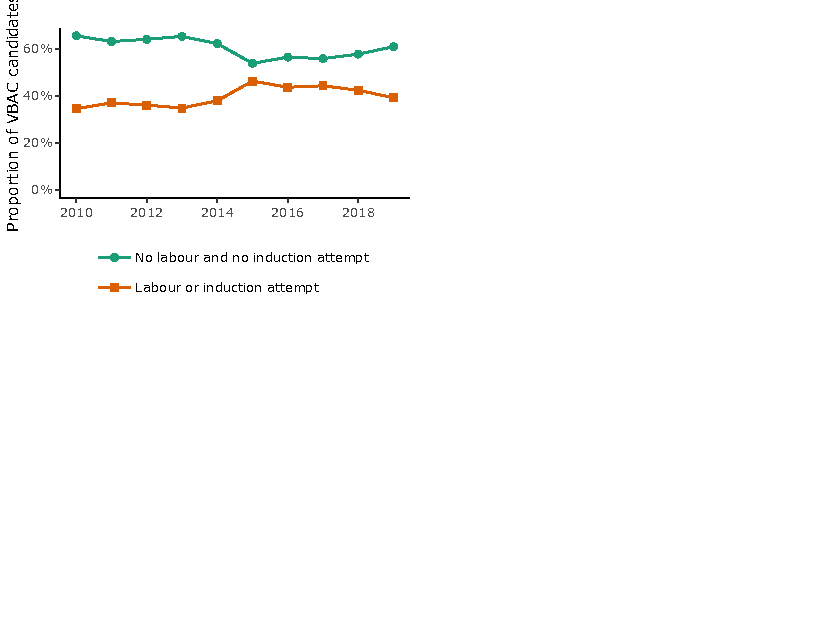
\includegraphics[width=0.9\linewidth,]{04-Labour_Birth_Process_files/figure-latex/plot49-1} \end{center}

\begin{table}[H]
\centering
\resizebox{\linewidth}{!}{
\begin{threeparttable}
\begin{tabular}[t]{lllllllllll}
\toprule
\textbf{} & \textbf{2011} & \textbf{2012} & \textbf{2013} & \textbf{2014} & \textbf{2015} & \textbf{2016} & \textbf{2017} & \textbf{2018} & \textbf{2019} & \textbf{2020}\\
\midrule
Total VBAC candidates & 809 & 824 & 813 & 926 & 822 & 858 & 789 & 803 & 811 & 793\\
No labour and no induction attempt & 63.7$\%$ & 64.7$\%$ & 65.4$\%$ & 62.1$\%$ & 55.0$\%$ & 58.4$\%$ & 56.3$\%$ & 59.2$\%$ & 61.9$\%$ & 62.9$\%$\\
Labour or induction attempt & 36.3$\%$ & 35.3$\%$ & 34.6$\%$ & 37.9$\%$ & 45.0$\%$ & 41.6$\%$ & 43.7$\%$ & 40.8$\%$ & 38.1$\%$ & 37.1$\%$\\
\bottomrule
\end{tabular}
\begin{tablenotes}
\item \textit{Note: } 
\item For the purposes of this report, a candidate for vaginal birth after Caesarean (VBAC) is woman who has had no more than one previous Caesarean section delivery; whose current pregnancy is a singleton in vertex presentation; and who has no contraindications for labour. On an individual basis when more information is available, such as type of previous Caesarean delivery, other factors are taken into account and women with two previous Caesarean deliveries may be considered for VBAC. \href{https://pubmed.ncbi.nlm.nih.gov/16001462/}{Ref: Society of Obstetricians and Gynaecologists of Canada. Guidelines for vaginal birth after previous caesarean birth. SOGC clinical practice guidelines. Number 155, February 2005. International Journal of Gynaecology and Obstetrics 2005;89(3):319-31}.
\end{tablenotes}
\end{threeparttable}}
\end{table}

\hypertarget{section-410}{%
\section{Type of delivery among candidates for vaginal birth after Caesarean (VBAC) who had any labour by year, 2011-2020}\label{section-410}}

\begin{center}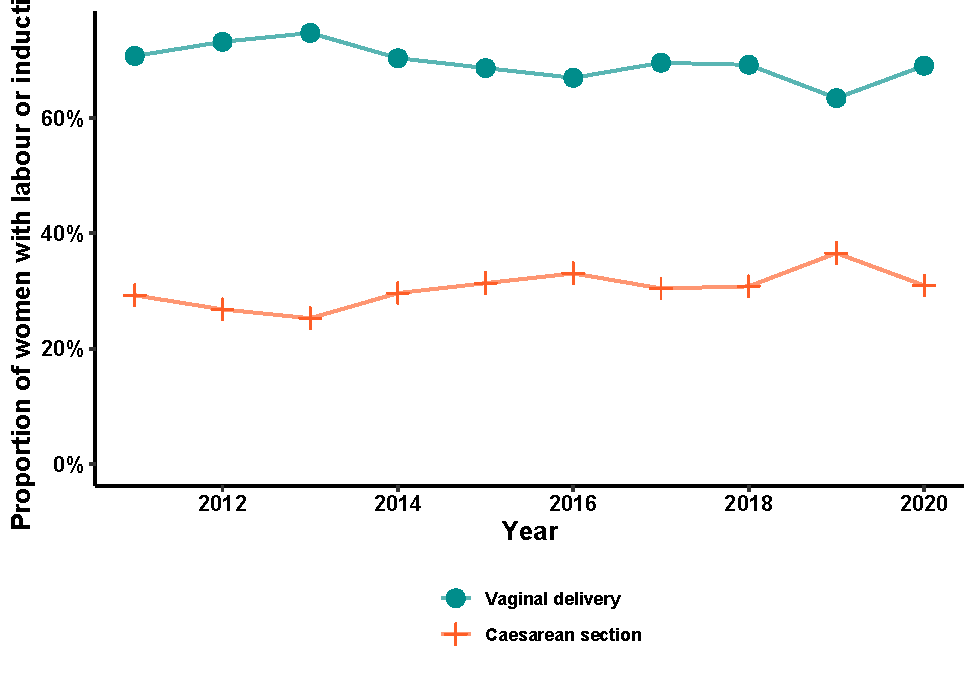
\includegraphics[width=0.9\linewidth,]{04-Labour_Birth_Process_files/figure-latex/plot410-1} \end{center}

\begin{table}[H]
\centering
\resizebox{\linewidth}{!}{
\begin{tabular}[t]{lllllllllll}
\toprule
\textbf{} & \textbf{2011} & \textbf{2012} & \textbf{2013} & \textbf{2014} & \textbf{2015} & \textbf{2016} & \textbf{2017} & \textbf{2018} & \textbf{2019} & \textbf{2020}\\
\midrule
Total women with labour or induction & 294 & 291 & 281 & 351 & 370 & 357 & 345 & 328 & 309 & 294\\
Vaginal delivery & 70.7$\%$ & 73.2$\%$ & 74.7$\%$ & 70.4$\%$ & 68.6$\%$ & 66.9$\%$ & 69.6$\%$ & 69.2$\%$ & 63.4$\%$ & 69.0$\%$\\
Caesarean section & 29.3$\%$ & 26.8$\%$ & 25.3$\%$ & 29.6$\%$ & 31.4$\%$ & 33.1$\%$ & 30.4$\%$ & 30.8$\%$ & 36.6$\%$ & 31.0$\%$\\
\bottomrule
\end{tabular}}
\end{table}

\hypertarget{section-411}{%
\section{Labour to 4 cm dilation among candidates for vaginal birth after Caesarean by year, 2011-2020}\label{section-411}}

\begin{center}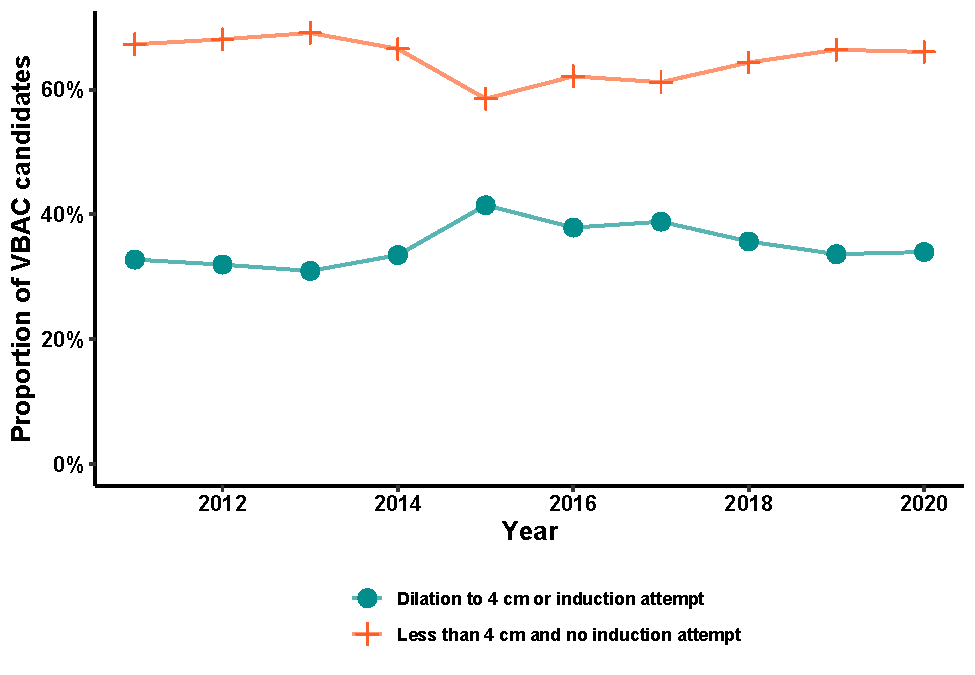
\includegraphics[width=0.9\linewidth,]{04-Labour_Birth_Process_files/figure-latex/plot411-1} \end{center}

\begin{table}[H]
\centering
\resizebox{\linewidth}{!}{
\begin{threeparttable}
\begin{tabular}[t]{lllllllllll}
\toprule
\textbf{} & \textbf{2011} & \textbf{2012} & \textbf{2013} & \textbf{2014} & \textbf{2015} & \textbf{2016} & \textbf{2017} & \textbf{2018} & \textbf{2019} & \textbf{2020}\\
\midrule
Total VBAC candidates\textsuperscript{a} & 803 & 820 & 805 & 920 & 815 & 850 & 783 & 788 & 803 & 789\\
Dilation to 4 cm or induction attempt & 32.8$\%$ & 32.0$\%$ & 30.9$\%$ & 33.5$\%$ & 41.5$\%$ & 37.9$\%$ & 38.8$\%$ & 35.7$\%$ & 33.6$\%$ & 34.0$\%$\\
Less than 4 cm and no induction attempt & 67.2$\%$ & 68.0$\%$ & 69.1$\%$ & 66.5$\%$ & 58.5$\%$ & 62.1$\%$ & 61.2$\%$ & 64.3$\%$ & 66.4$\%$ & 66.0$\%$\\
\bottomrule
\end{tabular}
\begin{tablenotes}
\item \textit{Note: } 
\item Women who are VBAC candidates and reach 4 cm cervical dilation may better represent those who have chosen to attempt a vaginal delivery. Intention to attempt a vaginal delivery is not recorded in the Atlee Database.
\item VBAC candidates with known cervical dilation who reached 4 cm.
\end{tablenotes}
\end{threeparttable}}
\end{table}

\hypertarget{section-412}{%
\section{Type of delivery among candidates for vaginal birth after Caesarean who had labour to 4 cm dilation by year, 2011-2020}\label{section-412}}

\begin{center}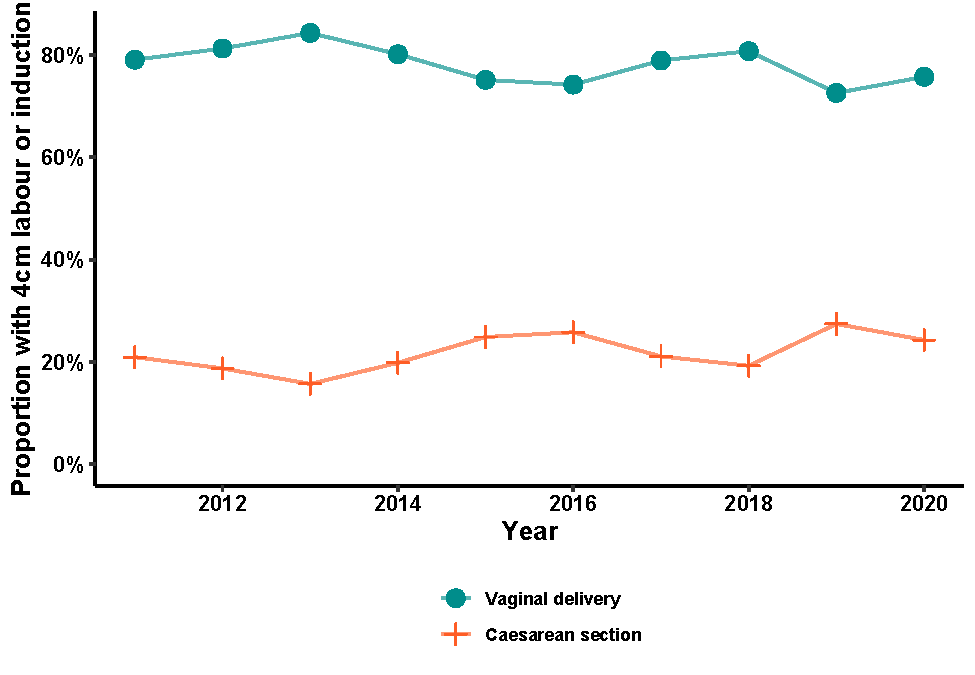
\includegraphics[width=0.9\linewidth,]{04-Labour_Birth_Process_files/figure-latex/plot412-1} \end{center}

\begin{table}[H]
\centering
\resizebox{\linewidth}{!}{
\begin{tabular}[t]{lllllllllll}
\toprule
\textbf{deliv} & \textbf{2011} & \textbf{2012} & \textbf{2013} & \textbf{2014} & \textbf{2015} & \textbf{2016} & \textbf{2017} & \textbf{2018} & \textbf{2019} & \textbf{2020}\\
\midrule
Total with 4 cm labour or induction & 263 & 262 & 249 & 308 & 338 & 322 & 304 & 281 & 270 & 268\\
Vaginal delivery & 79.1$\%$ & 81.3$\%$ & 84.3$\%$ & 80.2$\%$ & 75.1$\%$ & 74.2$\%$ & 78.9$\%$ & 80.8$\%$ & 72.6$\%$ & 75.7$\%$\\
Caesarean section & 20.9$\%$ & 18.7$\%$ & 15.7$\%$ & 19.8$\%$ & 24.9$\%$ & 25.8$\%$ & 21.1$\%$ & 19.2$\%$ & 27.4$\%$ & 24.3$\%$\\
\bottomrule
\end{tabular}}
\end{table}

\hypertarget{section-413}{%
\section{Episiotomy by parity and year, 2011-2020}\label{section-413}}

\begin{center}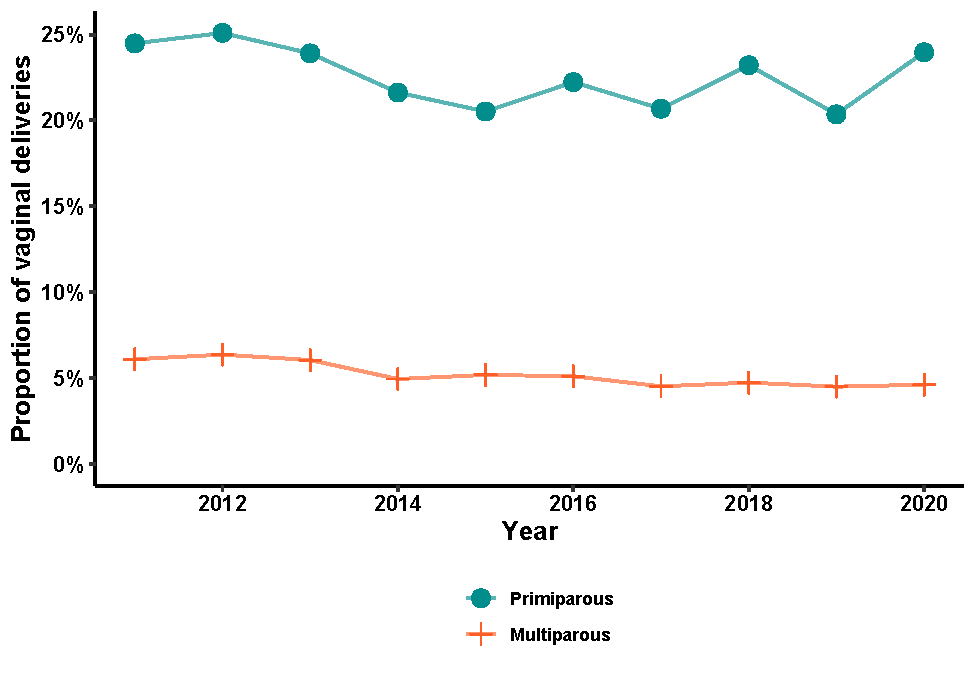
\includegraphics[width=0.9\linewidth,]{04-Labour_Birth_Process_files/figure-latex/plot413-1} \end{center}

\begin{table}[H]
\centering
\resizebox{\linewidth}{!}{
\begin{threeparttable}
\begin{tabular}[t]{lllllllllll}
\toprule
\textbf{Parity} & \textbf{2011} & \textbf{2012} & \textbf{2013} & \textbf{2014} & \textbf{2015} & \textbf{2016} & \textbf{2017} & \textbf{2018} & \textbf{2019} & \textbf{2020}\\
\midrule
\cellcolor[HTML]{E1E1E1}{\textbf{Primiparous}} & \cellcolor[HTML]{E1E1E1}{\textbf{}} & \cellcolor[HTML]{E1E1E1}{\textbf{}} & \cellcolor[HTML]{E1E1E1}{\textbf{}} & \cellcolor[HTML]{E1E1E1}{\textbf{}} & \cellcolor[HTML]{E1E1E1}{\textbf{}} & \cellcolor[HTML]{E1E1E1}{\textbf{}} & \cellcolor[HTML]{E1E1E1}{\textbf{}} & \cellcolor[HTML]{E1E1E1}{\textbf{}} & \cellcolor[HTML]{E1E1E1}{\textbf{}} & \cellcolor[HTML]{E1E1E1}{\textbf{}}\\
Total vaginal deliveries & 2,883 & 2,937 & 2,702 & 2,756 & 2,578 & 2,577 & 2,524 & 2,300 & 2,392 & 2,140\\
Episiotomy ($\%$) & 24.5$\%$ & 25.1$\%$ & 23.9$\%$ & 21.6$\%$ & 20.5$\%$ & 22.2$\%$ & 20.7$\%$ & 23.2$\%$ & 20.4$\%$ & 24.0$\%$\\
\cellcolor[HTML]{E1E1E1}{\textbf{Multiparous}} & \cellcolor[HTML]{E1E1E1}{\textbf{}} & \cellcolor[HTML]{E1E1E1}{\textbf{}} & \cellcolor[HTML]{E1E1E1}{\textbf{}} & \cellcolor[HTML]{E1E1E1}{\textbf{}} & \cellcolor[HTML]{E1E1E1}{\textbf{}} & \cellcolor[HTML]{E1E1E1}{\textbf{}} & \cellcolor[HTML]{E1E1E1}{\textbf{}} & \cellcolor[HTML]{E1E1E1}{\textbf{}} & \cellcolor[HTML]{E1E1E1}{\textbf{}} & \cellcolor[HTML]{E1E1E1}{\textbf{}}\\
Total vaginal deliveries & 3,526 & 3,440 & 3,371 & 3,496 & 3,375 & 3,405 & 3,429 & 3,356 & 3,242 & 3,077\\
Episiotomy ($\%$) & 6.1$\%$ & 6.4$\%$ & 6.1$\%$ & 4.9$\%$ & 5.2$\%$ & 5.1$\%$ & 4.5$\%$ & 4.7$\%$ & 4.5$\%$ & 4.6$\%$\\
\bottomrule
\end{tabular}
\begin{tablenotes}
\item \textit{Note: } 
\item An episiotomy is a mediolateral or midline incision made in the perineum during childbirth.
\end{tablenotes}
\end{threeparttable}}
\end{table}

\hypertarget{section-414}{%
\section{Obstetrical intervention by year, 2011-2020}\label{section-414}}

\begin{center}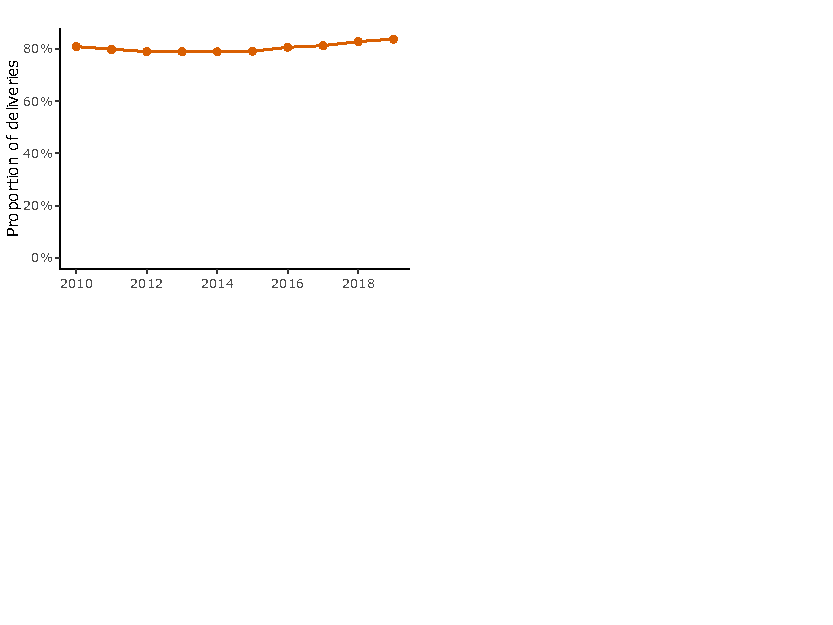
\includegraphics[width=0.9\linewidth,]{04-Labour_Birth_Process_files/figure-latex/plot414-1} \end{center}

\begin{table}[H]
\centering
\resizebox{\linewidth}{!}{
\begin{threeparttable}
\begin{tabular}[t]{lllllllllll}
\toprule
\textbf{Parity} & \textbf{2011} & \textbf{2012} & \textbf{2013} & \textbf{2014} & \textbf{2015} & \textbf{2016} & \textbf{2017} & \textbf{2018} & \textbf{2019} & \textbf{2020}\\
\midrule
Total deliveries & 8,771 & 8,619 & 8,327 & 8,521 & 8,054 & 8,198 & 8,116 & 7,834 & 7,939 & 7,490\\
Obstetrical intervention ($\%$) & 79.6$\%$ & 78.7$\%$ & 78.6$\%$ & 78.8$\%$ & 78.9$\%$ & 80.4$\%$ & 81.1$\%$ & 82.6$\%$ & 83.8$\%$ & 85.3$\%$\\
\bottomrule
\end{tabular}
\begin{tablenotes}
\item \textit{Note: } 
\item Obstetrical intervention includes the use of any of: induction, medical augmentation, anesthesia, Caesarean delivery, vaginal delivery involving the use of forceps and/or vacuum, or episiotomy.
\end{tablenotes}
\end{threeparttable}}
\end{table}

\hypertarget{section-5}{%
\chapter{Maternal Health Outcomes}\label{section-5}}

\hypertarget{section-51}{%
\section{Gestational diabetes by year, Nova Scotia, 2011-2020}\label{section-51}}

\begin{center}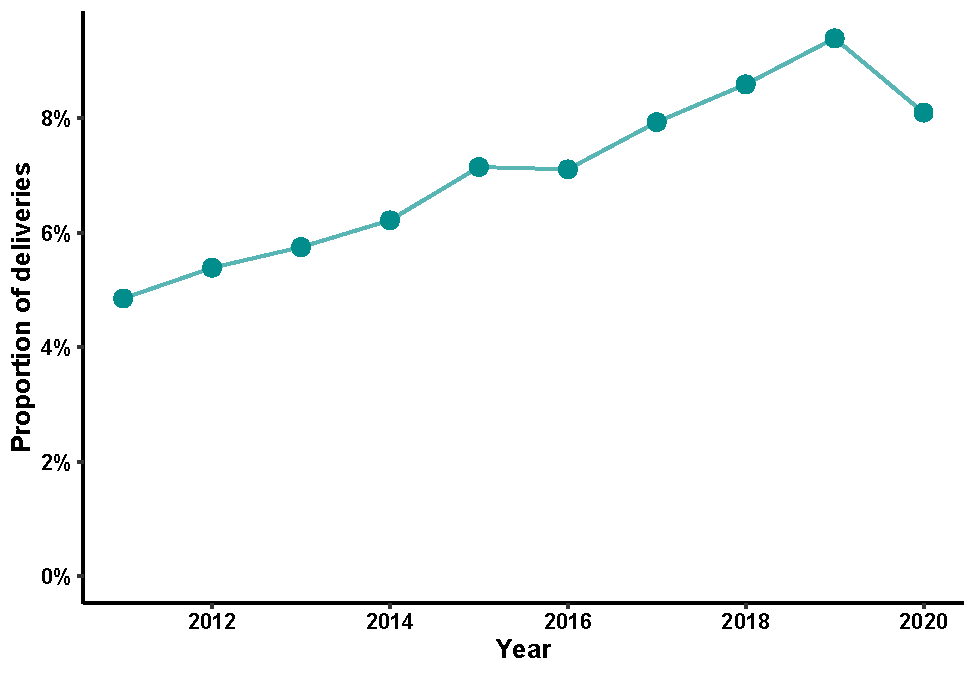
\includegraphics[width=0.9\linewidth,]{05-MHO_files/figure-latex/plot51-1} \end{center}

\begin{table}[H]
\centering
\resizebox{\linewidth}{!}{
\begin{threeparttable}
\begin{tabular}[t]{lllllllllll}
\toprule
\textbf{} & \textbf{2011} & \textbf{2012} & \textbf{2013} & \textbf{2014} & \textbf{2015} & \textbf{2016} & \textbf{2017} & \textbf{2018} & \textbf{2019} & \textbf{2020}\\
\midrule
Total deliveries\textsuperscript{a} & 8,672 & 8,553 & 8,258 & 8,424 & 7,985 & 8,087 & 8,014 & 7,736 & 7,830 & 7,394\\
Gestational diabetes ($\%$) & 4.9$\%$ & 5.4$\%$ & 5.8$\%$ & 6.2$\%$ & 7.2$\%$ & 7.1$\%$ & 7.9$\%$ & 8.6$\%$ & 9.4$\%$ & 8.1$\%$\\
\bottomrule
\end{tabular}
\begin{tablenotes}
\item \textit{Note: } 
\item Diabetes mellitus first detected in pregnancy as recorded in the medical record. Please note that the criteria for the diagnosis of gestational diabetes were revised by Diabetes Canada (formerly the Canadian Diabetes Association) in 2013. Therefore, the rates of gestational diabetes were expected to increase as the new criteria are adopted across Nova Scotia, starting approximately in late 2014.
\item[a] Among women without pre-existing diabetes.
\end{tablenotes}
\end{threeparttable}}
\end{table}

\hypertarget{section-52}{%
\section{Gestational hypertension by year, Nova Scotia, 2011-2020}\label{section-52}}

\begin{center}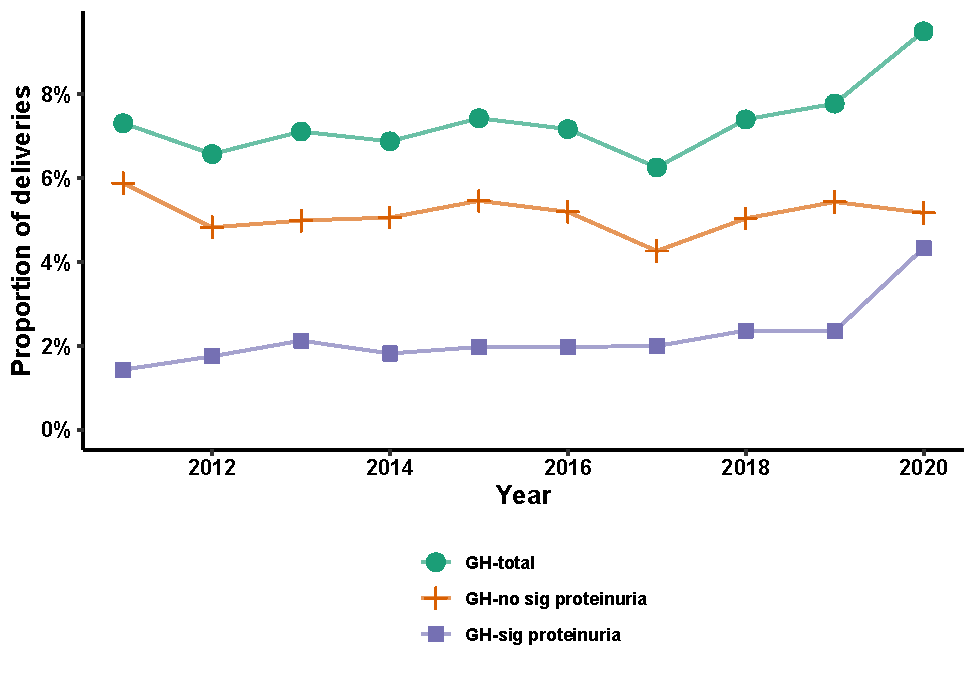
\includegraphics[width=0.9\linewidth,]{05-MHO_files/figure-latex/plot52-1} \end{center}

\begin{table}[H]
\centering
\resizebox{\linewidth}{!}{
\begin{threeparttable}
\begin{tabular}[t]{lllllllllll}
\toprule
\textbf{} & \textbf{2011} & \textbf{2012} & \textbf{2013} & \textbf{2014} & \textbf{2015} & \textbf{2016} & \textbf{2017} & \textbf{2018} & \textbf{2019} & \textbf{2020}\\
\midrule
Total deliveries\textsuperscript{a} & 8,668 & 8,514 & 8,236 & 8,415 & 7,964 & 8,099 & 8,021 & 7,738 & 7,839 & 7,384\\
GH-no sig proteinuria & 5.9$\%$ & 4.8$\%$ & 5.0$\%$ & 5.1$\%$ & 5.5$\%$ & 5.2$\%$ & 4.3$\%$ & 5.0$\%$ & 5.4$\%$ & 5.2$\%$\\
GH-sig proteinuria & 1.4$\%$ & 1.8$\%$ & 2.1$\%$ & 1.8$\%$ & 2.0$\%$ & 2.0$\%$ & 2.0$\%$ & 2.4$\%$ & 2.3$\%$ & 4.3$\%$\\
GH-total & 7.3$\%$ & 6.6$\%$ & 7.1$\%$ & 6.9$\%$ & 7.4$\%$ & 7.2$\%$ & 6.3$\%$ & 7.4$\%$ & 7.8$\%$ & 9.5$\%$\\
\bottomrule
\end{tabular}
\begin{tablenotes}
\item \textit{Note: } 
\item Gestational hypertension is hypertension that is first detected after the 20th week of gestation. Gestational hypertension with significant proteinuria includes those cases denoted as such; severe pre-eclampsia; HELLP syndrome (Hemolysis, Elevated Liver Enzymes, Low Platelets); and eclampsia.
\item[a] Among women without pre-existing hypertension.
\end{tablenotes}
\end{threeparttable}}
\end{table}

\hypertarget{section-53}{%
\section{Pre-eclampsia by year, Nova Scotia, 2011-2020}\label{section-53}}

\begin{center}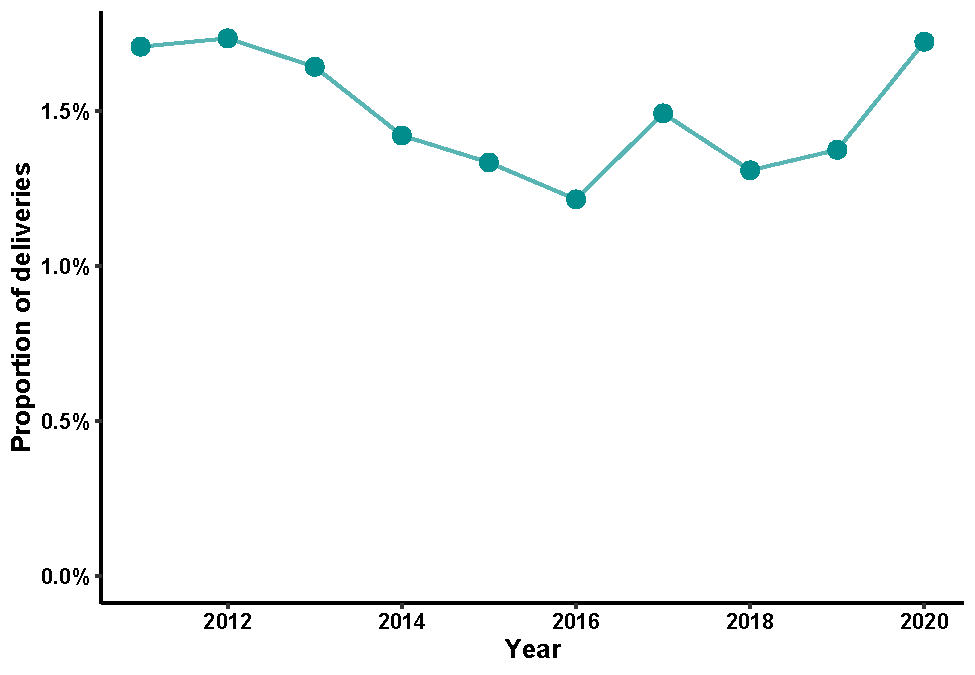
\includegraphics[width=0.9\linewidth,]{05-MHO_files/figure-latex/plot53-1} \end{center}

\begin{table}[H]
\centering
\resizebox{\linewidth}{!}{
\begin{threeparttable}
\begin{tabular}[t]{lllllllllll}
\toprule
\textbf{} & \textbf{2011} & \textbf{2012} & \textbf{2013} & \textbf{2014} & \textbf{2015} & \textbf{2016} & \textbf{2017} & \textbf{2018} & \textbf{2019} & \textbf{2020}\\
\midrule
Total deliveries & 8,899 & 8,760 & 8,460 & 8,651 & 8,167 & 8,308 & 8,237 & 7,942 & 8,070 & 7,599\\
Pre-eclampsia ($\%$) & 1.71$\%$ & 1.74$\%$ & 1.64$\%$ & 1.42$\%$ & 1.33$\%$ & 1.22$\%$ & 1.49$\%$ & 1.31$\%$ & 1.38$\%$ & 1.72$\%$\\
\bottomrule
\end{tabular}
\begin{tablenotes}
\item \textit{Note: } 
\item Pre-eclampsia includes women coded as having gestational hypertension with significant proteinuria, moderate or severe pre-eclampsia, HELLP syndrome (Hemolysis, Elevated Liver Enzymes, Low Platelets), eclampsia, or pre-existing hypertension with superimposed proteinuria.
\end{tablenotes}
\end{threeparttable}}
\end{table}

\hypertarget{section-54}{%
\section{Placenta previa by year, Nova Scotia, 2011-2020}\label{section-54}}

\begin{center}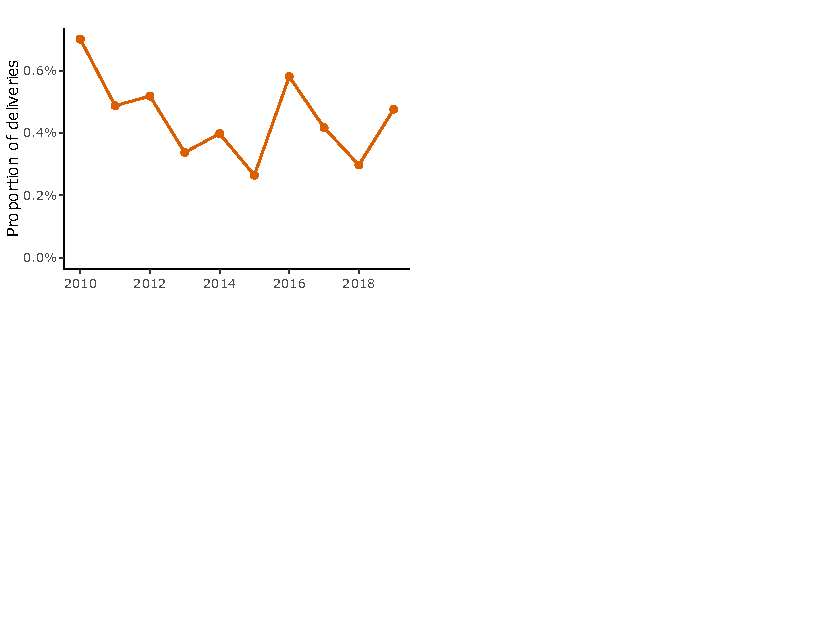
\includegraphics[width=0.9\linewidth,]{05-MHO_files/figure-latex/plot54-1} \end{center}

\begin{table}[H]
\centering
\resizebox{\linewidth}{!}{
\begin{threeparttable}
\begin{tabular}[t]{lllllllllll}
\toprule
\textbf{} & \textbf{2011} & \textbf{2012} & \textbf{2013} & \textbf{2014} & \textbf{2015} & \textbf{2016} & \textbf{2017} & \textbf{2018} & \textbf{2019} & \textbf{2020}\\
\midrule
Total deliveries & 8,764 & 8,618 & 8,325 & 8,514 & 8,051 & 8,194 & 8,111 & 7,832 & 7,938 & 7,491\\
Placenta previa ($\%$) & 0.49$\%$ & 0.52$\%$ & 0.32$\%$ & 0.39$\%$ & 0.26$\%$ & 0.57$\%$ & 0.41$\%$ & 0.24$\%$ & 0.47$\%$ & 0.68$\%$\\
\bottomrule
\end{tabular}
\begin{tablenotes}
\item \textit{Note: } 
\item Placenta previa is diagnosed when the placenta entirely or partially covers the opening of the uterus (cervix). The diagnosis is not made on ultrasound alone and must be confirmed clinically.
\end{tablenotes}
\end{threeparttable}}
\end{table}

\hypertarget{section-55}{%
\section{Placental abruption by year, Nova Scotia, 2011-2020}\label{section-55}}

\begin{center}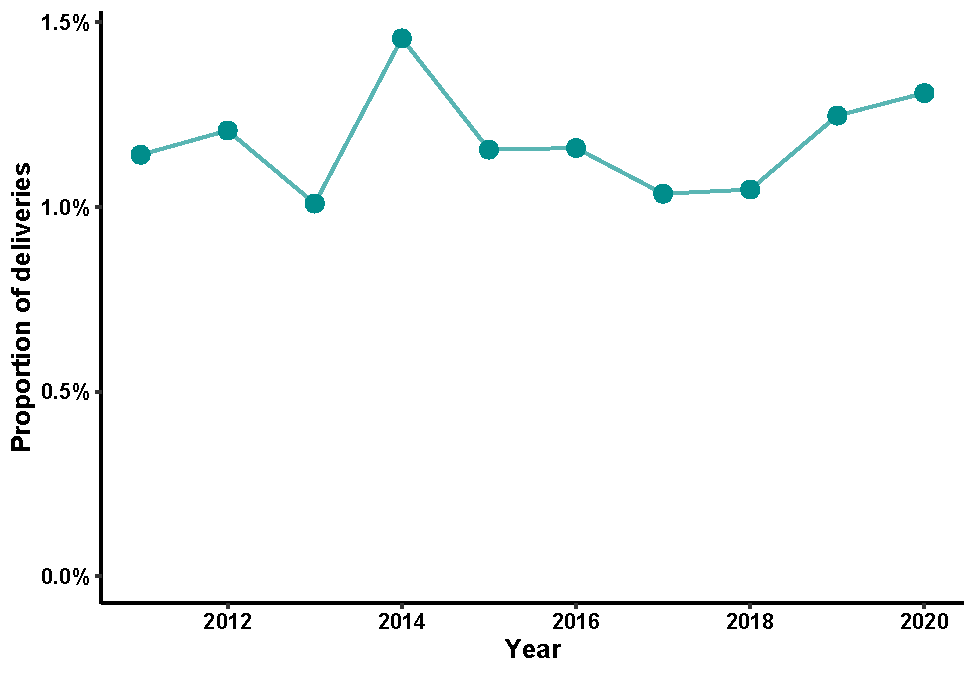
\includegraphics[width=0.9\linewidth,]{05-MHO_files/figure-latex/plot55-1} \end{center}

\begin{table}[H]
\centering
\resizebox{\linewidth}{!}{
\begin{threeparttable}
\begin{tabular}[t]{lllllllllll}
\toprule
\textbf{} & \textbf{2011} & \textbf{2012} & \textbf{2013} & \textbf{2014} & \textbf{2015} & \textbf{2016} & \textbf{2017} & \textbf{2018} & \textbf{2019} & \textbf{2020}\\
\midrule
Total deliveries & 8,764 & 8,618 & 8,325 & 8,514 & 8,051 & 8,194 & 8,111 & 7,832 & 7,938 & 7,491\\
Placenta abruption ($\%$) & 1.14$\%$ & 1.21$\%$ & 1.01$\%$ & 1.46$\%$ & 1.16$\%$ & 1.16$\%$ & 1.04$\%$ & 1.05$\%$ & 1.25$\%$ & 1.31$\%$\\
\bottomrule
\end{tabular}
\begin{tablenotes}
\item \textit{Note: } 
\item Placental abruption is defined as bleeding from the placental site due to the partial or complete separation of the placenta. The diagnosis is not made on ultrasound alone and must be confirmed clinically.
\end{tablenotes}
\end{threeparttable}}
\end{table}

\hypertarget{section-56}{%
\section{Perineal laceration deliveries by parity and year, Nova Scotia, 2011-2020}\label{section-56}}

\begin{center}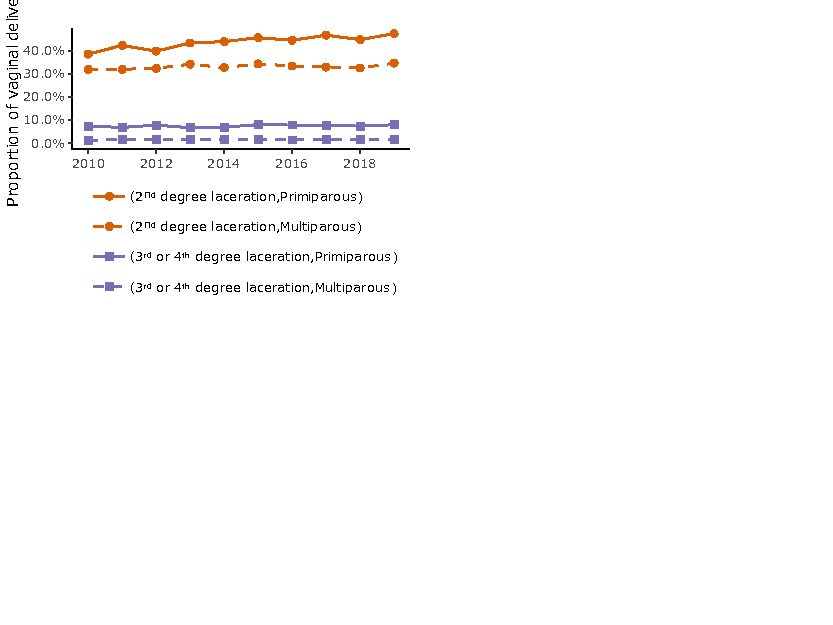
\includegraphics[width=0.9\linewidth,]{05-MHO_files/figure-latex/plot56-1} \end{center}

\begin{table}[H]
\centering
\resizebox{\linewidth}{!}{
\begin{threeparttable}
\begin{tabular}[t]{lllllllllll}
\toprule
\textbf{} & \textbf{2011} & \textbf{2012} & \textbf{2013} & \textbf{2014} & \textbf{2015} & \textbf{2016} & \textbf{2017} & \textbf{2018} & \textbf{2019} & \textbf{2020}\\
\midrule
\cellcolor[HTML]{E1E1E1}{\textbf{Primiparous}} & \cellcolor[HTML]{E1E1E1}{\textbf{}} & \cellcolor[HTML]{E1E1E1}{\textbf{}} & \cellcolor[HTML]{E1E1E1}{\textbf{}} & \cellcolor[HTML]{E1E1E1}{\textbf{}} & \cellcolor[HTML]{E1E1E1}{\textbf{}} & \cellcolor[HTML]{E1E1E1}{\textbf{}} & \cellcolor[HTML]{E1E1E1}{\textbf{}} & \cellcolor[HTML]{E1E1E1}{\textbf{}} & \cellcolor[HTML]{E1E1E1}{\textbf{}} & \cellcolor[HTML]{E1E1E1}{\textbf{}}\\
Total vaginal deliveries\textsuperscript{a} & 2,883 & 2,937 & 2,702 & 2,756 & 2,578 & 2,577 & 2,524 & 2,300 & 2,392 & 2,140\\
$2^{nd}$ degree laceration & 42.4$\%$ & 39.7$\%$ & 43.2$\%$ & 44.4$\%$ & 45.7$\%$ & 44.5$\%$ & 46.7$\%$ & 44.7$\%$ & 47.2$\%$ & 48.5$\%$\\
$3^{rd}$ or $4^{th}$ degree laceration & 7.0$\%$ & 8.1$\%$ & 6.9$\%$ & 7.1$\%$ & 8.2$\%$ & 8.1$\%$ & 7.6$\%$ & 7.6$\%$ & 8.0$\%$ & 8.4$\%$\\
\cellcolor[HTML]{E1E1E1}{\textbf{Multiparous}} & \cellcolor[HTML]{E1E1E1}{\textbf{}} & \cellcolor[HTML]{E1E1E1}{\textbf{}} & \cellcolor[HTML]{E1E1E1}{\textbf{}} & \cellcolor[HTML]{E1E1E1}{\textbf{}} & \cellcolor[HTML]{E1E1E1}{\textbf{}} & \cellcolor[HTML]{E1E1E1}{\textbf{}} & \cellcolor[HTML]{E1E1E1}{\textbf{}} & \cellcolor[HTML]{E1E1E1}{\textbf{}} & \cellcolor[HTML]{E1E1E1}{\textbf{}} & \cellcolor[HTML]{E1E1E1}{\textbf{}}\\
Total vaginal deliveries\textsuperscript{a} & 3,526 & 3,440 & 3,371 & 3,496 & 3,375 & 3,404 & 3,429 & 3,356 & 3,242 & 3,077\\
$2^{nd}$ degree laceration & 32.0$\%$ & 32.6$\%$ & 34.2$\%$ & 32.9$\%$ & 34.4$\%$ & 33.3$\%$ & 33.0$\%$ & 32.7$\%$ & 34.8$\%$ & 34.7$\%$\\
$3^{rd}$ or $4^{th}$ degree laceration & 1.9$\%$ & 1.6$\%$ & 1.7$\%$ & 1.6$\%$ & 1.8$\%$ & 1.5$\%$ & 1.9$\%$ & 1.8$\%$ & 1.9$\%$ & 1.7$\%$\\
\bottomrule
\end{tabular}
\begin{tablenotes}
\item \textit{Note: } 
\item Maternal perineal laceration, rupture or tear during delivery involving the pelvic floor, perineal muscles, or vaginal muscles ($2^{nd}$ degree), anal sphincter ($3^{rd}$ degree), or rectal mucosa ($4^{th}$ degree).
\end{tablenotes}
\end{threeparttable}}
\end{table}

\hypertarget{section-58}{%
\section{Postpartum hemorrhage by year, Nova Scotia, 2011-2020}\label{section-58}}

\begin{center}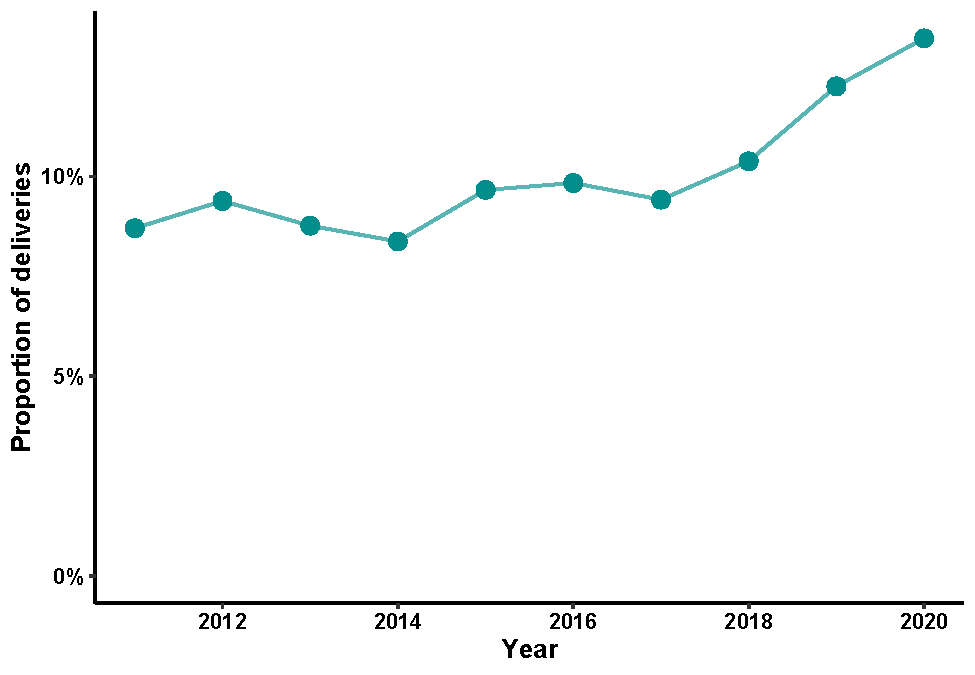
\includegraphics[width=0.9\linewidth,]{05-MHO_files/figure-latex/plot58-1} \end{center}

\begin{table}[H]
\centering
\resizebox{\linewidth}{!}{
\begin{threeparttable}
\begin{tabular}[t]{lllllllllll}
\toprule
\textbf{} & \textbf{2011} & \textbf{2012} & \textbf{2013} & \textbf{2014} & \textbf{2015} & \textbf{2016} & \textbf{2017} & \textbf{2018} & \textbf{2019} & \textbf{2020}\\
\midrule
Total deliveries & 8,764 & 8,618 & 8,325 & 8,514 & 8,051 & 8,194 & 8,111 & 7,832 & 7,938 & 7,491\\
Postpartum hemorrhage ($\%$) & 8.7$\%$ & 9.4$\%$ & 8.8$\%$ & 8.4$\%$ & 9.7$\%$ & 9.8$\%$ & 9.4$\%$ & 10.4$\%$ & 12.3$\%$ & 13.5$\%$\\
\bottomrule
\end{tabular}
\begin{tablenotes}
\item \textit{Note: } 
\item Postpartum hemorrhage is diagnosed if, after the delivery of the fetus, excessive maternal bleeding occurs from the genital tract with an estimated blood loss of greater than 500 mL for vaginal deliveries or 1000 mL for Caesarean section deliveries.
\end{tablenotes}
\end{threeparttable}}
\end{table}

\hypertarget{section-59}{%
\section{Maternal blood transfusion by year, Nova Scotia, 2011-2020}\label{section-59}}

\begin{center}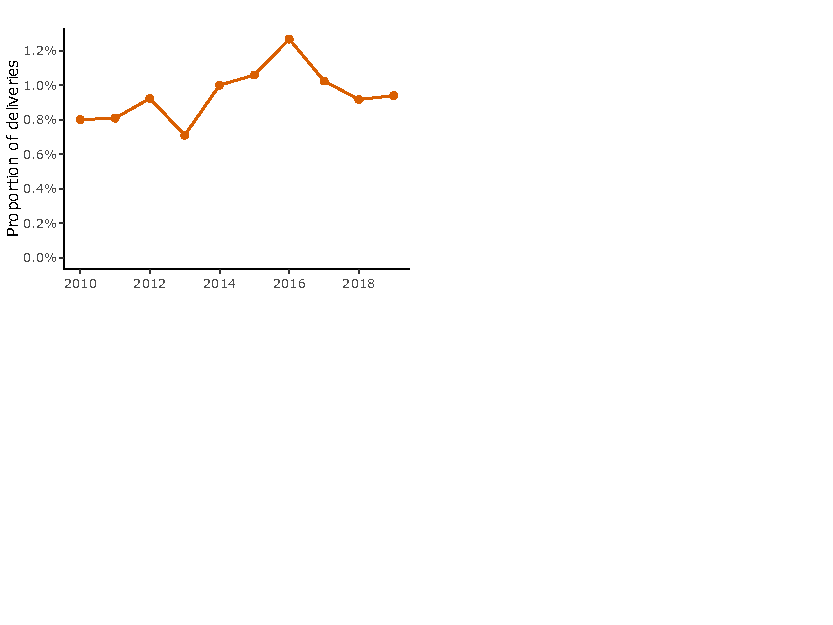
\includegraphics[width=0.9\linewidth,]{05-MHO_files/figure-latex/plot59-1} \end{center}

\begin{table}[H]
\centering
\resizebox{\linewidth}{!}{
\begin{threeparttable}
\begin{tabular}[t]{lllllllllll}
\toprule
\textbf{} & \textbf{2011} & \textbf{2012} & \textbf{2013} & \textbf{2014} & \textbf{2015} & \textbf{2016} & \textbf{2017} & \textbf{2018} & \textbf{2019} & \textbf{2020}\\
\midrule
Total deliveries & 8,764 & 8,618 & 8,325 & 8,514 & 8,051 & 8,194 & 8,111 & 7,832 & 7,938 & 7,491\\
Transfusion ($\%$) & 0.80$\%$ & 0.91$\%$ & 0.70$\%$ & 0.94$\%$ & 0.99$\%$ & 1.13$\%$ & 0.92$\%$ & 0.82$\%$ & 0.89$\%$ & 0.93$\%$\\
\bottomrule
\end{tabular}
\begin{tablenotes}
\item \textit{Note: } 
\item One or more maternal transfusions of red blood cells in the antepartum, intrapartum, or postpartum periods.
\end{tablenotes}
\end{threeparttable}}
\end{table}

\hypertarget{section-510}{%
\section{Maternal antepartum hospital length of stay (in hours) by year, Nova Scotia, 2011-2020}\label{section-510}}

\begin{center}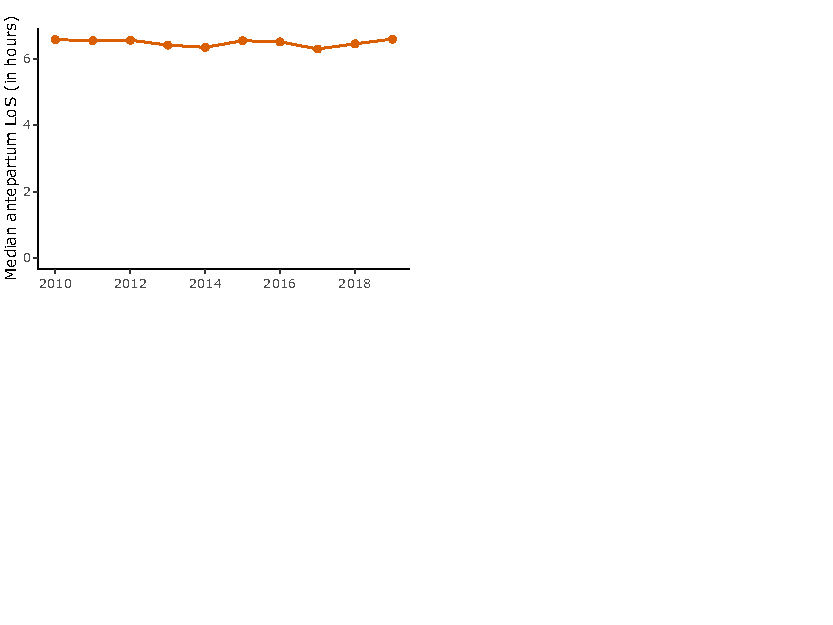
\includegraphics[width=0.9\linewidth,]{05-MHO_files/figure-latex/plot510-1} \end{center}

\begin{table}[H]
\centering
\resizebox{\linewidth}{!}{
\begin{tabular}[t]{lllllllllll}
\toprule
\textbf{} & \textbf{2011} & \textbf{2012} & \textbf{2013} & \textbf{2014} & \textbf{2015} & \textbf{2016} & \textbf{2017} & \textbf{2018} & \textbf{2019} & \textbf{2020}\\
\midrule
Total deliveries & 8,899 & 8,760 & 8,460 & 8,651 & 8,167 & 8,308 & 8,237 & 7,942 & 8,070 & 7,599\\
Mean (in hours) & 17.1 & 17.0 & 17.1 & 16.6 & 15.8 & 13.1 & 13.2 & 12.3 & 13.6 & 13.9\\
Median (in hours) & 6.5 & 6.5 & 6.4 & 6.3 & 6.5 & 6.5 & 6.3 & 6.4 & 6.6 & 7.2\\
\bottomrule
\end{tabular}}
\end{table}

\hypertarget{section-511}{%
\section{Maternal postpartum hospital length of stay (in hours) by type of delivery and year, Nova Scotia, 2011-2020}\label{section-511}}

\begin{center}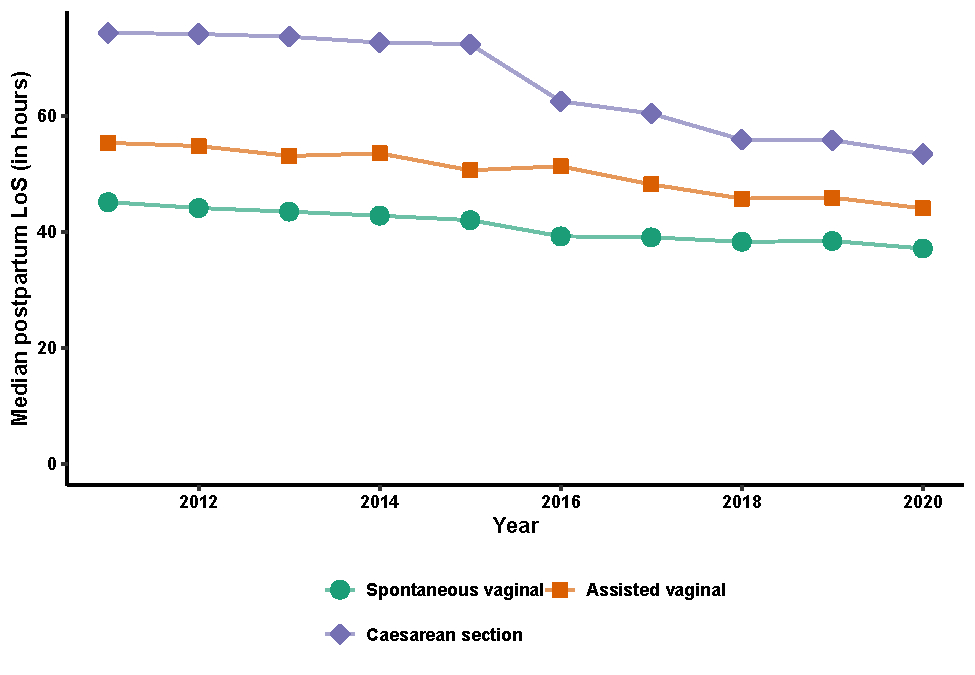
\includegraphics[width=0.9\linewidth,]{05-MHO_files/figure-latex/plot511-1} \end{center}

\begin{table}[H]
\centering
\resizebox{\linewidth}{!}{
\begin{tabular}[t]{lllllllllll}
\toprule
\textbf{} & \textbf{2011} & \textbf{2012} & \textbf{2013} & \textbf{2014} & \textbf{2015} & \textbf{2016} & \textbf{2017} & \textbf{2018} & \textbf{2019} & \textbf{2020}\\
\midrule
\cellcolor[HTML]{E1E1E1}{\textbf{Spontenaous vaginal}} & \cellcolor[HTML]{E1E1E1}{\textbf{}} & \cellcolor[HTML]{E1E1E1}{\textbf{}} & \cellcolor[HTML]{E1E1E1}{\textbf{}} & \cellcolor[HTML]{E1E1E1}{\textbf{}} & \cellcolor[HTML]{E1E1E1}{\textbf{}} & \cellcolor[HTML]{E1E1E1}{\textbf{}} & \cellcolor[HTML]{E1E1E1}{\textbf{}} & \cellcolor[HTML]{E1E1E1}{\textbf{}} & \cellcolor[HTML]{E1E1E1}{\textbf{}} & \cellcolor[HTML]{E1E1E1}{\textbf{}}\\
Total deliveries & 5,700 & 5,714 & 5,472 & 5,640 & 5,349 & 5,331 & 5,253 & 4,962 & 4,898 & 4,552\\
Mean (in hours) & 50.0 & 48.7 & 47.6 & 47.3 & 48.4 & 46.7 & 46.5 & 44.5 & 45.1 & 43.7\\
Median (in hours) & 45.1 & 44.1 & 43.5 & 42.8 & 42.0 & 39.2 & 39.0 & 38.3 & 38.4 & 37.1\\
\cellcolor[HTML]{E1E1E1}{\textbf{Assisted vaginal}} & \cellcolor[HTML]{E1E1E1}{\textbf{}} & \cellcolor[HTML]{E1E1E1}{\textbf{}} & \cellcolor[HTML]{E1E1E1}{\textbf{}} & \cellcolor[HTML]{E1E1E1}{\textbf{}} & \cellcolor[HTML]{E1E1E1}{\textbf{}} & \cellcolor[HTML]{E1E1E1}{\textbf{}} & \cellcolor[HTML]{E1E1E1}{\textbf{}} & \cellcolor[HTML]{E1E1E1}{\textbf{}} & \cellcolor[HTML]{E1E1E1}{\textbf{}} & \cellcolor[HTML]{E1E1E1}{\textbf{}}\\
Total deliveries & 771 & 727 & 654 & 676 & 649 & 704 & 756 & 742 & 783 & 706\\
Mean (in hours) & 61.7 & 61.2 & 59.5 & 61.5 & 59.1 & 59.9 & 56.3 & 53.9 & 53.2 & 53.6\\
Median (in hours) & 55.3 & 54.8 & 53.1 & 53.5 & 50.6 & 51.3 & 48.2 & 45.7 & 45.9 & 44.0\\
\cellcolor[HTML]{E1E1E1}{\textbf{Caesarean section}} & \cellcolor[HTML]{E1E1E1}{\textbf{}} & \cellcolor[HTML]{E1E1E1}{\textbf{}} & \cellcolor[HTML]{E1E1E1}{\textbf{}} & \cellcolor[HTML]{E1E1E1}{\textbf{}} & \cellcolor[HTML]{E1E1E1}{\textbf{}} & \cellcolor[HTML]{E1E1E1}{\textbf{}} & \cellcolor[HTML]{E1E1E1}{\textbf{}} & \cellcolor[HTML]{E1E1E1}{\textbf{}} & \cellcolor[HTML]{E1E1E1}{\textbf{}} & \cellcolor[HTML]{E1E1E1}{\textbf{}}\\
Total deliveries & 2,427 & 2,319 & 2,334 & 2,334 & 2,169 & 2,272 & 2,227 & 2,237 & 2,389 & 2,341\\
Mean (in hours) & 77.3 & 77.2 & 75.9 & 74.5 & 76.8 & 69.9 & 69.2 & 65.7 & 65.9 & 62.2\\
Median (in hours) & 74.3 & 74.1 & 73.7 & 72.6 & 72.4 & 62.5 & 60.4 & 55.9 & 55.8 & 53.4\\
\bottomrule
\end{tabular}}
\end{table}

\hypertarget{section-6}{%
\chapter{Fetal and Infant Health Outcomes}\label{section-6}}

\hypertarget{section-61}{%
\section{Low birth weight by year, Nova Scotia, 2011-2020}\label{section-61}}

\begin{center}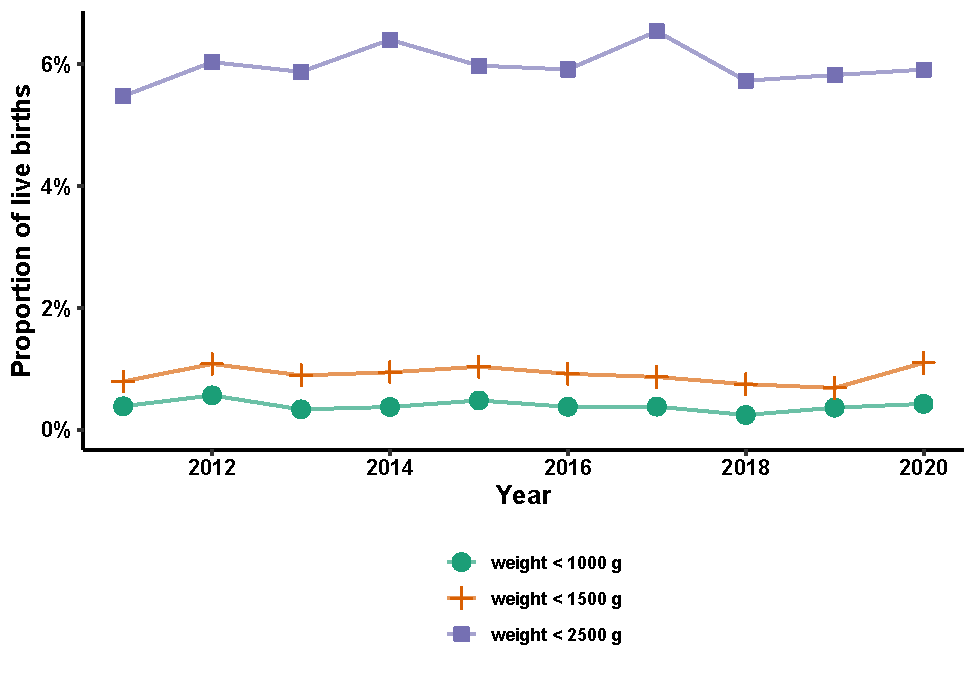
\includegraphics[width=0.9\linewidth,]{06-FIHO_files/figure-latex/plot61-1} \end{center}

\begin{table}[H]
\centering
\resizebox{\linewidth}{!}{
\begin{threeparttable}
\begin{tabular}[t]{lllllllllll}
\toprule
\textbf{} & \textbf{2011} & \textbf{2012} & \textbf{2013} & \textbf{2014} & \textbf{2015} & \textbf{2016} & \textbf{2017} & \textbf{2018} & \textbf{2019} & \textbf{2020}\\
\midrule
Total live births\textsuperscript{a} & 8,860 & 8,720 & 8,429 & 8,609 & 8,135 & 8,289 & 8,214 & 7,909 & 8,041 & 7,564\\
weight < 1000 g & 0.38$\%$ & 0.56$\%$ & 0.33$\%$ & 0.37$\%$ & 0.48$\%$ & 0.37$\%$ & 0.38$\%$ & 0.24$\%$ & 0.36$\%$ & 0.42$\%$\\
weight < 1500 g & 0.79$\%$ & 1.08$\%$ & 0.89$\%$ & 0.94$\%$ & 1.03$\%$ & 0.92$\%$ & 0.86$\%$ & 0.75$\%$ & 0.68$\%$ & 1.10$\%$\\
weight < 2500 g & 5.47$\%$ & 6.03$\%$ & 5.87$\%$ & 6.40$\%$ & 5.97$\%$ & 5.91$\%$ & 6.54$\%$ & 5.73$\%$ & 5.82$\%$ & 5.91$\%$\\
\bottomrule
\end{tabular}
\begin{tablenotes}
\item[a] With known birth weight.
\end{tablenotes}
\end{threeparttable}}
\end{table}

\hypertarget{section-62}{%
\section{Macrosomia by year, Nova Scotia, 2011-2020}\label{section-62}}

\begin{center}\includegraphics[width=0.9\linewidth,]{06-FIHO_files/figure-latex/plot62-1} \end{center}

\begin{table}[H]
\centering
\resizebox{\linewidth}{!}{
\begin{threeparttable}
\begin{tabular}[t]{lllllllllll}
\toprule
\textbf{} & \textbf{2011} & \textbf{2012} & \textbf{2013} & \textbf{2014} & \textbf{2015} & \textbf{2016} & \textbf{2017} & \textbf{2018} & \textbf{2019} & \textbf{2020}\\
\midrule
Total live births\textsuperscript{a} & 8,860 & 8,720 & 8,429 & 8,609 & 8,135 & 8,289 & 8,214 & 7,909 & 8,041 & 7,564\\
weight > 4000 g & 13.6$\%$ & 13.1$\%$ & 13.3$\%$ & 12.4$\%$ & 11.6$\%$ & 12.3$\%$ & 11.6$\%$ & 11.9$\%$ & 10.5$\%$ & 11.6$\%$\\
weight > 4500 g & 1.9$\%$ & 2.2$\%$ & 2.1$\%$ & 1.9$\%$ & 1.8$\%$ & 2.1$\%$ & 1.7$\%$ & 1.8$\%$ & 1.4$\%$ & 1.8$\%$\\
\bottomrule
\end{tabular}
\begin{tablenotes}
\item[a] With known birth weight.
\end{tablenotes}
\end{threeparttable}}
\end{table}

\hypertarget{section-63}{%
\section{Small for gestational age by year, Nova Scotia, 2011-2020}\label{section-63}}

\begin{center}\includegraphics[width=0.9\linewidth,]{06-FIHO_files/figure-latex/plot63-1} \end{center}

\begin{table}[H]
\centering
\resizebox{\linewidth}{!}{
\begin{threeparttable}
\begin{tabular}[t]{lllllllllll}
\toprule
\textbf{} & \textbf{2011} & \textbf{2012} & \textbf{2013} & \textbf{2014} & \textbf{2015} & \textbf{2016} & \textbf{2017} & \textbf{2018} & \textbf{2019} & \textbf{2020}\\
\midrule
Total live births\textsuperscript{a} & 8,832 & 8,681 & 8,407 & 8,584 & 8,114 & 8,277 & 8,204 & 7,907 & 8,030 & 7,556\\
< $3^{rd}$ percentile & 2.5$\%$ & 2.4$\%$ & 2.4$\%$ & 2.5$\%$ & 2.2$\%$ & 2.5$\%$ & 2.4$\%$ & 2.0$\%$ & 2.4$\%$ & 2.4$\%$\\
< $10^{th}$ percentile & 8.3$\%$ & 8.2$\%$ & 8.7$\%$ & 8.5$\%$ & 8.6$\%$ & 8.7$\%$ & 9.2$\%$ & 8.5$\%$ & 9.3$\%$ & 8.6$\%$\\
\bottomrule
\end{tabular}
\begin{tablenotes}
\item \textit{Note: } 
\item Size for gestational age is based on sex-specific percentiles of birth weight for gestational age relative to a Canadian reference population \href{https://publications.aap.org/pediatrics/article/108/2/e35/63679/A-New-and-Improved-Population-Based-Canadian?autologincheck=redirected'}{Ref: Kramer et al. A New and Improved Population-Based Canadian Reference for Birth Weight for Gestational Age. Pediatrics 2001; 108 (2):e35}.
\item[a] With known birth weight.
\end{tablenotes}
\end{threeparttable}}
\end{table}

\hypertarget{section-64}{%
\section{Large for gestational age by year, Nova Scotia, 2011-2020}\label{section-64}}

\begin{center}\includegraphics[width=0.9\linewidth,]{06-FIHO_files/figure-latex/plot64-1} \end{center}

\begin{table}[H]
\centering
\resizebox{\linewidth}{!}{
\begin{threeparttable}
\begin{tabular}[t]{lllllllllll}
\toprule
\textbf{} & \textbf{2011} & \textbf{2012} & \textbf{2013} & \textbf{2014} & \textbf{2015} & \textbf{2016} & \textbf{2017} & \textbf{2018} & \textbf{2019} & \textbf{2020}\\
\midrule
Total live births\textsuperscript{a} & 8,832 & 8,681 & 8,407 & 8,584 & 8,114 & 8,277 & 8,204 & 7,907 & 8,030 & 7,556\\
$\geq 90^{th}$ percentile & 14.0$\%$ & 13.4$\%$ & 12.8$\%$ & 12.5$\%$ & 12.0$\%$ & 12.7$\%$ & 11.7$\%$ & 12.5$\%$ & 11.6$\%$ & 12.8$\%$\\
$\geq 97^{th}$ percentile & 4.4$\%$ & 4.6$\%$ & 4.3$\%$ & 4.1$\%$ & 3.8$\%$ & 4.5$\%$ & 3.6$\%$ & 3.9$\%$ & 3.6$\%$ & 4.1$\%$\\
\bottomrule
\end{tabular}
\begin{tablenotes}
\item \textit{Note: } 
\item Size for gestational age is based on sex-specific percentiles of birth weight for gestational age relative to a Canadian reference population \href{https://publications.aap.org/pediatrics/article/108/2/e35/63679/A-New-and-Improved-Population-Based-Canadian?autologincheck=redirected'}{Ref: Kramer et al. A New and Improved Population-Based Canadian Reference for Birth Weight for Gestational Age. Pediatrics 2001; 108 (2):e35}.
\item[a] With known birth weight.
\end{tablenotes}
\end{threeparttable}}
\end{table}

\hypertarget{section-65}{%
\section{Preterm births by year, Nova Scotia, 2011-2020}\label{section-65}}

\begin{center}\includegraphics[width=0.9\linewidth,]{06-FIHO_files/figure-latex/plot65-1} \end{center}

\begin{table}[H]
\centering
\resizebox{\linewidth}{!}{
\begin{threeparttable}
\begin{tabular}[t]{lllllllllll}
\toprule
\textbf{} & \textbf{2011} & \textbf{2012} & \textbf{2013} & \textbf{2014} & \textbf{2015} & \textbf{2016} & \textbf{2017} & \textbf{2018} & \textbf{2019} & \textbf{2020}\\
\midrule
Total live births\textsuperscript{a} & 8,846 & 8,698 & 8,417 & 8,597 & 8,124 & 8,286 & 8,210 & 7,909 & 8,039 & 7,563\\
< 28 weeks & 0.3$\%$ & 0.5$\%$ & 0.3$\%$ & 0.4$\%$ & 0.4$\%$ & 0.4$\%$ & 0.4$\%$ & 0.2$\%$ & 0.4$\%$ & 0.5$\%$\\
< 32 weeks & 0.9$\%$ & 1.1$\%$ & 1.2$\%$ & 1.3$\%$ & 1.3$\%$ & 1.2$\%$ & 1.1$\%$ & 1.0$\%$ & 0.9$\%$ & 1.2$\%$\\
< 34 weeks & 1.6$\%$ & 2.1$\%$ & 2.0$\%$ & 2.3$\%$ & 2.1$\%$ & 2.0$\%$ & 2.1$\%$ & 1.8$\%$ & 1.8$\%$ & 1.9$\%$\\
< 37 weeks & 7.4$\%$ & 7.9$\%$ & 8.0$\%$ & 8.5$\%$ & 8.7$\%$ & 8.4$\%$ & 8.6$\%$ & 8.2$\%$ & 8.1$\%$ & 7.9$\%$\\
\bottomrule
\end{tabular}
\begin{tablenotes}
\item \textit{Note: } 
\item The derivation of gestational age is primarily based on the date of the mother's last menstrual period (LMP). If LMP is unknown or LMP-estimated gestational age is discordant with that estimated by early fetal ultrasound measurements, then gestational age based on early fetal ultrasound measurements is used. If early fetal ultrasound measurements are unavailable and gestational age based on LMP is discordant from that clinically estimated by the neonatal physical exam, then the clinically estimated gestational age is used.
\item[a] With known gestational age.
\end{tablenotes}
\end{threeparttable}}
\end{table}

\hypertarget{section-66}{%
\section{Birth injury by year, Nova Scotia, 2011-2020}\label{section-66}}

\begin{center}\includegraphics[width=0.9\linewidth,]{06-FIHO_files/figure-latex/plot66-1} \end{center}

\begin{table}[H]
\centering
\resizebox{\linewidth}{!}{
\begin{threeparttable}
\begin{tabular}[t]{lllllllllll}
\toprule
\textbf{} & \textbf{2011} & \textbf{2012} & \textbf{2013} & \textbf{2014} & \textbf{2015} & \textbf{2016} & \textbf{2017} & \textbf{2018} & \textbf{2019} & \textbf{2020}\\
\midrule
Total live births & 8,863 & 8,722 & 8,434 & 8,612 & 8,138 & 8,294 & 8,216 & 7,911 & 8,046 & 7,567\\
Birth injury ($\%$) & 0.42$\%$ & 0.26$\%$ & 0.30$\%$ & 0.35$\%$ & 0.25$\%$ & 0.30$\%$ & 0.37$\%$ & 0.46$\%$ & 0.15$\%$ & 0.25$\%$\\
\bottomrule
\end{tabular}
\begin{tablenotes}
\item \textit{Note: } 
\item Any injury to the infant occurring during delivery such as fracture (e.g., femur, clavicle, rib, humerus, depressed skull) or central nervous system trauma (e.g., cerebral hemorrhage, spinal cord hemorrhage, brachial plexus palsy).
\end{tablenotes}
\end{threeparttable}}
\end{table}

\hypertarget{section-67}{%
\section{Phototherapy by year, Nova Scotia, 2011-2020}\label{section-67}}

\begin{center}\includegraphics[width=0.9\linewidth,]{06-FIHO_files/figure-latex/plot67-1} \end{center}

\begin{table}[H]
\centering
\resizebox{\linewidth}{!}{
\begin{threeparttable}
\begin{tabular}[t]{lllllllllll}
\toprule
\textbf{} & \textbf{2011} & \textbf{2012} & \textbf{2013} & \textbf{2014} & \textbf{2015} & \textbf{2016} & \textbf{2017} & \textbf{2018} & \textbf{2019} & \textbf{2020}\\
\midrule
Total live births & 8,863 & 8,722 & 8,434 & 8,612 & 8,138 & 8,294 & 8,216 & 7,911 & 8,046 & 7,567\\
Received phototerapy ($\%$) & 17.5$\%$ & 15.5$\%$ & 13.2$\%$ & 12.9$\%$ & 13.0$\%$ & 13.2$\%$ & 15.1$\%$ & 11.6$\%$ & 10.9$\%$ & 11.8$\%$\\
\bottomrule
\end{tabular}
\begin{tablenotes}
\item \textit{Note: } 
\item Phototherapy involves exposure of the neonate to coloured light in hospital (birth hospital or readmission in the neonatal period). It is given for known or suspected hyperbilirubinemia (jaundice).
\end{tablenotes}
\end{threeparttable}}
\end{table}

\hypertarget{section-68}{%
\section{Type of respiratory distress syndrome by year, Nova Scotia, 2011-2020}\label{section-68}}

\begin{center}\includegraphics[width=0.9\linewidth,]{06-FIHO_files/figure-latex/plot68-1} \end{center}

\begin{table}[H]
\centering
\resizebox{\linewidth}{!}{
\begin{threeparttable}
\begin{tabular}[t]{lllllllllll}
\toprule
\textbf{} & \textbf{2011} & \textbf{2012} & \textbf{2013} & \textbf{2014} & \textbf{2015} & \textbf{2016} & \textbf{2017} & \textbf{2018} & \textbf{2019} & \textbf{2020}\\
\midrule
Total live births & 8,863 & 8,722 & 8,434 & 8,612 & 8,138 & 8,294 & 8,216 & 7,911 & 8,046 & 7,567\\
Mild & 0.58$\%$ & 0.62$\%$ & 0.49$\%$ & 0.51$\%$ & 0.45$\%$ & 0.46$\%$ & 0.45$\%$ & 0.63$\%$ & 0.43$\%$ & 0.41$\%$\\
Moderate & 0.12$\%$ & 0.14$\%$ & 0.12$\%$ & 0.12$\%$ & 0.10$\%$ & 0.12$\%$ & 0.16$\%$ & 0.08$\%$ & 0.07$\%$ & 0.00$\%$\\
Severe & 0.28$\%$ & 0.33$\%$ & 0.20$\%$ & 0.16$\%$ & 0.12$\%$ & 0.18$\%$ & 0.12$\%$ & 0.10$\%$ & 0.15$\%$ & 0.15$\%$\\
TTN\textsuperscript{a} & 1.44$\%$ & 1.18$\%$ & 1.86$\%$ & 1.47$\%$ & 1.57$\%$ & 1.84$\%$ & 1.57$\%$ & 1.88$\%$ & 2.40$\%$ & 2.31$\%$\\
Unknown severity & 1.49$\%$ & 1.71$\%$ & 1.99$\%$ & 1.79$\%$ & 1.89$\%$ & 1.62$\%$ & 2.00$\%$ & 2.22$\%$ & 2.25$\%$ & 2.99$\%$\\
\cellcolor[HTML]{E1E1E1}{\textbf{Total RDS}} & \cellcolor[HTML]{E1E1E1}{\textbf{3.92$\%$}} & \cellcolor[HTML]{E1E1E1}{\textbf{3.98$\%$}} & \cellcolor[HTML]{E1E1E1}{\textbf{4.66$\%$}} & \cellcolor[HTML]{E1E1E1}{\textbf{4.05$\%$}} & \cellcolor[HTML]{E1E1E1}{\textbf{4.14$\%$}} & \cellcolor[HTML]{E1E1E1}{\textbf{4.22$\%$}} & \cellcolor[HTML]{E1E1E1}{\textbf{4.30$\%$}} & \cellcolor[HTML]{E1E1E1}{\textbf{4.92$\%$}} & \cellcolor[HTML]{E1E1E1}{\textbf{5.31$\%$}} & \cellcolor[HTML]{E1E1E1}{\textbf{5.85$\%$}}\\
\bottomrule
\end{tabular}
\begin{tablenotes}
\item \textit{Note: } 
\item Respiratory distress syndrome (RDS) is identified by neonatal grunting, retractions, and decreased air entry that occur before 3 hours of age, persist beyond 6 hours of age, and are not explained by any other disease. Severity is categorized by the treatment given by the physician as noted in the medical record: mild, < 35\% oxygen; moderate, 35\% oxygen or continuous positive airway pressure (CPAP); severe, ventilated. Note that as medical practice changes with respect to the type of treatment given, the proportion of RDS that is of unknown severity may increase.
\item[a] TTN = Transient tachypnea of the newborn.
\end{tablenotes}
\end{threeparttable}}
\end{table}

\hypertarget{section-69}{%
\section{Neonatal sepsis by birth weight and year, Nova Scotia, 2011-2020}\label{section-69}}

\begin{center}\includegraphics[width=0.9\linewidth,]{06-FIHO_files/figure-latex/plot69-1} \end{center}

\begin{table}[H]
\centering
\resizebox{\linewidth}{!}{
\begin{threeparttable}
\begin{tabular}[t]{lllllllllll}
\toprule
\textbf{Birth weight} & \textbf{2011} & \textbf{2012} & \textbf{2013} & \textbf{2014} & \textbf{2015} & \textbf{2016} & \textbf{2017} & \textbf{2018} & \textbf{2019} & \textbf{2020}\\
\midrule
\cellcolor[HTML]{E1E1E1}{\textbf{weight < 1000 g}} & \cellcolor[HTML]{E1E1E1}{\textbf{}} & \cellcolor[HTML]{E1E1E1}{\textbf{}} & \cellcolor[HTML]{E1E1E1}{\textbf{}} & \cellcolor[HTML]{E1E1E1}{\textbf{}} & \cellcolor[HTML]{E1E1E1}{\textbf{}} & \cellcolor[HTML]{E1E1E1}{\textbf{}} & \cellcolor[HTML]{E1E1E1}{\textbf{}} & \cellcolor[HTML]{E1E1E1}{\textbf{}} & \cellcolor[HTML]{E1E1E1}{\textbf{}} & \cellcolor[HTML]{E1E1E1}{\textbf{}}\\
Total live births & 34 & 49 & 28 & 32 & 39 & 31 & 31 & 19 & 29 & 32\\
Neonatal sepsis ($\%$) & 20.6$\%$ & 26.5$\%$ & 21.4$\%$ & 53.1$\%$ & 33.3$\%$ & 25.8$\%$ & 45.2$\%$ & 36.8$\%$ & 37.9$\%$ & 40.6$\%$\\
\cellcolor[HTML]{E1E1E1}{\textbf{1000 g $\leq$ weight < 2500 g}} & \cellcolor[HTML]{E1E1E1}{\textbf{}} & \cellcolor[HTML]{E1E1E1}{\textbf{}} & \cellcolor[HTML]{E1E1E1}{\textbf{}} & \cellcolor[HTML]{E1E1E1}{\textbf{}} & \cellcolor[HTML]{E1E1E1}{\textbf{}} & \cellcolor[HTML]{E1E1E1}{\textbf{}} & \cellcolor[HTML]{E1E1E1}{\textbf{}} & \cellcolor[HTML]{E1E1E1}{\textbf{}} & \cellcolor[HTML]{E1E1E1}{\textbf{}} & \cellcolor[HTML]{E1E1E1}{\textbf{}}\\
Total live births & 451 & 477 & 467 & 519 & 447 & 459 & 506 & 434 & 439 & 415\\
Neonatal sepsis ($\%$) & 2.4$\%$ & 4.2$\%$ & 2.1$\%$ & 2.7$\%$ & 3.4$\%$ & 2.6$\%$ & 2.2$\%$ & 4.4$\%$ & 2.1$\%$ & 4.1$\%$\\
\cellcolor[HTML]{E1E1E1}{\textbf{weight $\geq$ 2500 g}} & \cellcolor[HTML]{E1E1E1}{\textbf{}} & \cellcolor[HTML]{E1E1E1}{\textbf{}} & \cellcolor[HTML]{E1E1E1}{\textbf{}} & \cellcolor[HTML]{E1E1E1}{\textbf{}} & \cellcolor[HTML]{E1E1E1}{\textbf{}} & \cellcolor[HTML]{E1E1E1}{\textbf{}} & \cellcolor[HTML]{E1E1E1}{\textbf{}} & \cellcolor[HTML]{E1E1E1}{\textbf{}} & \cellcolor[HTML]{E1E1E1}{\textbf{}} & \cellcolor[HTML]{E1E1E1}{\textbf{}}\\
Total live births & 8,375 & 8,194 & 7,934 & 8,058 & 7,649 & 7,799 & 7,677 & 7,456 & 7,573 & 7,117\\
Neonatal sepsis ($\%$) & 0.33$\%$ & 0.55$\%$ & 0.39$\%$ & 0.37$\%$ & 0.68$\%$ & 0.53$\%$ & 0.38$\%$ & 0.64$\%$ & 0.67$\%$ & 0.37$\%$\\
\bottomrule
\end{tabular}
\begin{tablenotes}
\item \textit{Note: } 
\item Pneumonia, either intrauterine or postnatal, or positive blood/cerebrospinal fluid cultures.
\end{tablenotes}
\end{threeparttable}}
\end{table}

\hypertarget{section-610}{%
\section{Newborn length of stay (in days) by birth weight and year, Nova Scotia, 2011-2020}\label{section-610}}

\begin{center}\includegraphics[width=0.9\linewidth,]{06-FIHO_files/figure-latex/plot610-1} \end{center}

\begin{table}[H]
\centering
\resizebox{\linewidth}{!}{
\begin{threeparttable}
\begin{tabular}[t]{lllllllllll}
\toprule
\textbf{Birth weight} & \textbf{2011} & \textbf{2012} & \textbf{2013} & \textbf{2014} & \textbf{2015} & \textbf{2016} & \textbf{2017} & \textbf{2018} & \textbf{2019} & \textbf{2020}\\
\midrule
\cellcolor[HTML]{E1E1E1}{\textbf{weight < 1000 g}} & \cellcolor[HTML]{E1E1E1}{\textbf{}} & \cellcolor[HTML]{E1E1E1}{\textbf{}} & \cellcolor[HTML]{E1E1E1}{\textbf{}} & \cellcolor[HTML]{E1E1E1}{\textbf{}} & \cellcolor[HTML]{E1E1E1}{\textbf{}} & \cellcolor[HTML]{E1E1E1}{\textbf{}} & \cellcolor[HTML]{E1E1E1}{\textbf{}} & \cellcolor[HTML]{E1E1E1}{\textbf{}} & \cellcolor[HTML]{E1E1E1}{\textbf{}} & \cellcolor[HTML]{E1E1E1}{\textbf{}}\\
Total births\textsuperscript{a} & 28 & 36 & 20 & 20 & 26 & 13 & 21 & 16 & 15 & 19\\
Mean (in days) & 84.6 & 98.5 & 119.1 & 124.9 & 97.2 & 112.8 & 108.8 & 91.4 & 93.2 & 90.8\\
Median (in days) & 74.6 & 101.3 & 97.4 & 112.6 & 101.1 & 107.7 & 109.0 & 81.3 & 89.5 & 102.6\\
\cellcolor[HTML]{E1E1E1}{\textbf{1000 g $\leq$ weight < 2500 g}} & \cellcolor[HTML]{E1E1E1}{\textbf{}} & \cellcolor[HTML]{E1E1E1}{\textbf{}} & \cellcolor[HTML]{E1E1E1}{\textbf{}} & \cellcolor[HTML]{E1E1E1}{\textbf{}} & \cellcolor[HTML]{E1E1E1}{\textbf{}} & \cellcolor[HTML]{E1E1E1}{\textbf{}} & \cellcolor[HTML]{E1E1E1}{\textbf{}} & \cellcolor[HTML]{E1E1E1}{\textbf{}} & \cellcolor[HTML]{E1E1E1}{\textbf{}} & \cellcolor[HTML]{E1E1E1}{\textbf{}}\\
Total births\textsuperscript{a} & 444 & 466 & 460 & 512 & 442 & 452 & 493 & 429 & 430 & 413\\
Mean (in days) & 14.1 & 15.7 & 17.7 & 17.4 & 16.0 & 16.0 & 14.0 & 15.4 & 14.1 & 16.1\\
Median (in days) & 6.0 & 8.3 & 7.7 & 7.3 & 6.5 & 6.2 & 5.4 & 6.2 & 7.0 & 5.9\\
\cellcolor[HTML]{E1E1E1}{\textbf{weight $\geq$ 2500 g}} & \cellcolor[HTML]{E1E1E1}{\textbf{}} & \cellcolor[HTML]{E1E1E1}{\textbf{}} & \cellcolor[HTML]{E1E1E1}{\textbf{}} & \cellcolor[HTML]{E1E1E1}{\textbf{}} & \cellcolor[HTML]{E1E1E1}{\textbf{}} & \cellcolor[HTML]{E1E1E1}{\textbf{}} & \cellcolor[HTML]{E1E1E1}{\textbf{}} & \cellcolor[HTML]{E1E1E1}{\textbf{}} & \cellcolor[HTML]{E1E1E1}{\textbf{}} & \cellcolor[HTML]{E1E1E1}{\textbf{}}\\
Total births\textsuperscript{a} & 8,366 & 8,189 & 7,927 & 8,050 & 7,641 & 7,785 & 7,660 & 7,448 & 7,561 & 7,109\\
Mean (in days) & 2.8 & 2.8 & 2.7 & 2.8 & 2.7 & 2.6 & 2.5 & 2.7 & 2.7 & 2.4\\
Median (in days) & 2.3 & 2.2 & 2.2 & 2.1 & 2.1 & 2.0 & 2.0 & 2.0 & 2.0 & 1.9\\
\bottomrule
\end{tabular}
\begin{tablenotes}
\item[a] Number of births of infants who survived to hospital discharge.
\end{tablenotes}
\end{threeparttable}}
\end{table}

\hypertarget{section-611}{%
\section{Neonatal withdrawal from maternal use of opioids by year, Nova Scotia, 2011-2020}\label{section-611}}

\begin{center}\includegraphics[width=0.9\linewidth,]{06-FIHO_files/figure-latex/plot611-1} \end{center}

\begin{table}[H]
\centering
\resizebox{\linewidth}{!}{
\begin{threeparttable}
\begin{tabular}[t]{lllllllllll}
\toprule
\textbf{} & \textbf{2011} & \textbf{2012} & \textbf{2013} & \textbf{2014} & \textbf{2015} & \textbf{2016} & \textbf{2017} & \textbf{2018} & \textbf{2019} & \textbf{2020}\\
\midrule
Total live births & 8,863 & 8,722 & 8,434 & 8,612 & 8,138 & 8,294 & 8,216 & 7,911 & 8,046 & 7,567\\
Neonatal withdrawal & 0.34$\%$ & 0.55$\%$ & 0.36$\%$ & 0.62$\%$ & 0.61$\%$ & 0.60$\%$ & 0.67$\%$ & 0.47$\%$ & 0.61$\%$ & 0.58$\%$\\
\bottomrule
\end{tabular}
\begin{tablenotes}
\item \textit{Note: } 
\item Neonatal withdrawal symptoms from maternal dependency on opioid drugs. Does not include neonatal reactions from opioid drugs administered to the mother during labour or delivery.
\end{tablenotes}
\end{threeparttable}}
\end{table}

\hypertarget{glossary}{%
\chapter*{Glossary}\label{glossary}}


\textbf{Assisted reproductive technology}

From records of the hospital delivery admission and can include assisted reproduction, ovulation induction, intracytoplasmic sperm injection (ICSI), embryo transfer, and \emph{in vitro} fertilization (IVF).

\textbf{Assisted vaginal delivery}

Vaginal delivery involving the use of forceps and/or vacuum.

\textbf{Birth}

Birth refers to the live born or stillborn infant. ``Births'' are differentiated from ``deliveries''. For example, a woman who had twins is counted as having one delivery and two births.

\textbf{Birth injury}

Any injury to the infant occurring during delivery such as fracture (e.g., femur, clavicle, rib, humerus, depressed skull) or central nervous system trauma (e.g., cerebral hemorrhage, spinal cord hemorrhage, brachial plexus palsy).

\textbf{Body mass index (BMI)}

Calculated as weight in kilograms divided by the square of height in metres.

\begin{itemize}
\tightlist
\item
  Underweight: \(BMI < 18.5 \, kg/m^{2}\)
\item
  Normal weight: \(18.5 \, kg/m^{2} \le BMI \le 24.9 \, kg/m^{2}\)
\item
  Overweight: \(25 \, kg/m^{2} \le BMI \le 29.9 \, kg/m^{2}\)
\item
  Obese: \(BMI \ge 30 \, kg/m^{2}\)
\end{itemize}

\textbf{Breastfeeding status}

Describes the method of infant feeding during the hospital stay. Breastfeeding refers to when the infant was given breast milk: Exclusive denotes that the infant received only breast milk and non-exclusive denotes that the infant received breast milk with supplementation.

\textbf{Caesarean section delivery}

Delivery of the fetus through an incision in the abdominal and uterine walls.
Cannabis use Use of cannabis in pregnancy if recorded on the Nova Scotia Prenatal Record.

\textbf{Delivery}

A delivery marks the end of pregnancy, regardless of the number of infants born. For example, a woman who had
twins is counted as having one delivery and two births.

\textbf{Early neonatal mortality}

Death of a liveborn infant, occurring up to the sixth completed day of life (6 days, 23 hours and 59 minutes).

\textbf{Episiotomy}

A mediolateral or midline incision made in the perineum during childbirth.

\textbf{Gestational age}

Gestational age is calculated from an algorithm that incorporates information from early ultrasound measurements (before 25 weeks), the first day of the last normal menstrual period (LMP), and a clinical estimate based on a physical examination of the infant shortly after birth. The derivation is primarily based on the date of the mother's last menstrual period (LMP). If LMP is unknown or LMP-estimated gestational age is discordant with that estimated by early fetal ultrasound measurements, then gestational age based on early fetal ultrasound measurements is used. If early fetal ultrasound measurements are unavailable and gestational age based on LMP is discordant from that clinically estimated by the neonatal physical exam, then the clinically estimated gestational age is used.

\textbf{Gestational diabetes}

Diabetes mellitus first detected in pregnancy as recorded in the medical record. Please note that the criteria for the diagnosis of gestational diabetes were revised by Diabetes Canada (formerly the Canadian Diabetes Association) in 2013. Therefore, the rates of gestational diabetes were expected to increase as the new criteria are adopted across Nova Scotia, starting approximately in late 2014. {[}Ref: Canadian Diabetes Association Clinical Practice Guidelines Expert Committee. Canadian Diabetes Association 2013 Clinical Practice Guidelines for the Prevention and Management of Diabetes in Canada. Canadian Journal of Diabetes. 2013;37(suppl1):S1-12{]}.

\textbf{Gestational hypertension}

Gestational hypertension is hypertension that is first detected after the 20th week of gestation. Gestational hypertension with significant proteinuria includes those cases denoted as such; severe pre-eclampsia; HELLP syndrome (Hemolysis, Elevated Liver Enzymes, Low Platelets); and eclampsia.

\textbf{Gestational weight gain}

Gestational weight gain guidelines set by the US Institute of Medicine and Health Canada are specific to a woman's pre-pregnancy BMI category: Underweight, 12.5 to 18 kg; Normal weight, 11.5 to 16 kg; Overweight, 7 to 11.5 kg; Obese, 5 to 9 kg.

\begin{itemize}
\tightlist
\item
  Inadequate: Below the recommended range.
\item
  Adequate: Within the recommended range.
\item
  Excessive: Above the recommended range.
\end{itemize}

\textbf{Indication for labour induction}

Reason for induction of labour as documented on the medical chart. The `Other medical reason' category includes maternal diabetes, maternal history of precipitate labour, pruritic uticarial papules and plaques of pregnancy (PUPP), thrombocytopenia, maternal seizure, vaginal bleeding, premature rupture of membranes with clinical
chorioamnionitis, isoimmunization, concern for fetal well being (abnormal biophysical profile, abnormal or atypical non-stress test, abnormal Doppler), oligohydramnios (decreased amniotic fluid), polyhydramnios (increased amniotic fluid), multiple pregnancy, and positive group B Streptococcus with rupture of membranes.

\textbf{Infant mortality}

Death of a liveborn infant occurring within the first year of life.

\textbf{Interpregnancy weight change}

Calculated as the pre-pregnancy weight in the index pregnancy minus the pre-pregnancy weight in the woman's preceding pregnancy.

\textbf{Labour induction}

The initiation of contractions in a pregnant woman who is not in labour to help her achieve a vaginal birth within 24 to 48 hours.

\textbf{Laceration}

Maternal perineal laceration, rupture or tear during delivery involving the pelvic floor, perineal muscles, or vaginal muscles (\(2^{nd}\) degree), anal sphincter (\(3^{rd}\) degree), or rectal mucosa (\(4^{th}\) degree).

\textbf{Large for gestational age}

See `Size for gestational age'.

\textbf{Live birth}

Live birth refers to birth of an infant with signs of life.

\textbf{Macrosomia}

Refers to birth weight beyond two specific thresholds, 4,000 g and 4,500 g. The American College of Obstetricians and Gynecologists supports use of the 4,500 g threshold for diagnosis of macrosomia because morbidity increases sharply beyond this weight, but acknowledges there is some increased risk of morbidity at weights \textgreater{} 4,000 g. {[}Ref: ACOG Practice Bulletin No.22: Fetal Macrosomia. American College of Obstetricians and Gynecologists, Washington DC 2000{]}

\textbf{Maternal antepartum hospital length of stay}

Hours between maternal admission to the birth facility and delivery.

\textbf{Maternal blood transfusion}

One or more maternal transfusions of red blood cells in the antepartum, intrapartum, or postpartum periods.

\textbf{Maternal postpartum hospital length of stay}
Hours between delivery and discharge of the mother from the birth facility.

\textbf{Medical augmentation}

Use of oxytocin to improve contractions after labour has started spontaneously.

\textbf{Neonatal mortality}

Death of a liveborn infant, occurring up to the 27th completed day of life (27 days, 23 hours and 59 minutes).

\textbf{Neonatal sepsis}

Isolation of bacterial or fungal or viral organism from blood or cerebrospinal fluid in the symptomatic infant. In addition to blood culture, this includes viral or fungal infection. This definition does not include congenital or postnatal pneumonia.

\textbf{Neonatal withdrawal}

Neonatal withdrawal symptoms from maternal dependency on opioid drugs. Does not include neonatal reactions from opioid drugs administered to the mother during labour or delivery.

\textbf{Newborn length of stay}

The total number of days a baby stayed in the delivery hospital and transfer hospital(s) (if applicable) before being discharged home. This calculation does not include newborns who have died in-hospital or who have not yet been discharged home.

\textbf{Obstetrical intervention}

A delivery that includes any of: induction, medical augmentation, anesthesia, caesarean delivery, vaginal delivery involving the use of forceps and/or vacuum, or episiotomy.

\textbf{Opioid agonist maintenance therapy}

Maternal use of methadone, buprenorphine, or other opioid agonist in pregnancy if recorded on the Nova Scotia Prenatal Record.

\textbf{Parity}

Number of pregnancies, excluding the present pregnancy, which resulted in the delivery of 1 or more infants weighing 500 g or more at birth (regardless of the outcome of such infants).

\textbf{Partner status}

Partnered denotes women who are married or in a common-law relationship.

\textbf{Perinatal mortality}

Death of an infant, occurring up to the sixth completed day of life (6 days, 23 hours and 59 minutes). Includes stillbirths and early neonatal deaths.

\textbf{Phototherapy}

Exposure of the neonate to coloured light in hospital (birth hospital or readmission in the neonatal period). Phototherapy is given for known or suspected hyperbilirubinemia (jaundice).

\textbf{Placenta previa}

Placenta entirely or partially covering the internal os. The diagnosis is not made on ultrasound alone and must be confirmed clinically.

\textbf{Placental abruption}

Bleeding from the placental site due to the partial or complete separation of the placenta. The diagnosis is not made on ultrasound alone and must be confirmed clinically.

\textbf{Postneonatal mortality}

Death of a liveborn infant weighing 500 g or more at birth, occurring from 28 days to 1 year of life.

\textbf{Postpartum hemorrhage}

After the delivery of the fetus, excessive maternal bleeding from the genital tract with an estimated blood loss of greater than 500 mL for vaginal deliveries or 1000 mL for Caesarean section deliveries.

\textbf{Pre-eclampsia}

Gestational hypertension with proteinuria, or pre-existing hypertension with superimposed proteinuria. Includes HELLP syndrome (Hemolysis, Elevated Liver Enzymes, Low Platelets).

\textbf{Pre-existing diabetes}

Maternal history of either Type 1 or Type 2 diabetes mellitus prior to the current pregnancy.

\textbf{Pre-existing hypertension}

Maternal history of hypertensive disease prior to the current pregnancy or prior to 20 weeks' gestation in the current pregnancy.

\textbf{Regional anesthesia}

Use of epidural, spinal, and/or pudendal anesthesia during labour and/or delivery.
Respiratory Distress Syndrome (RDS) Grunting, retractions, and decreased air entry - occurring before 3 hours of age and persisting beyond 6 hours of age and not explained by any other disease. Severity of RDS is categorized by the treatment given by the physician as recorded in the medical record:

\begin{itemize}
\tightlist
\item
  Mild: \textless{} 35\% oxygen
\item
  Moderate: 35\% oxygen or continuous positive airway pressure (CPAP)
\item
  Severe: Ventilated
\item
  TTN: Transient tachypnea of the newborn
\end{itemize}

Note that as medical practice changes with respect to the type of treatment given, the proportion of RDS that is of unknown severity will increase.

\textbf{Robson group}

The Robson criteria for the classification of deliveries into ten mutually exclusive groups by maternal characteristics allows comparison of Caesarean section rates at regional and national levels. Please note that for the purposes of this report:

\begin{enumerate}
\def\labelenumi{\arabic{enumi}.}
\tightlist
\item
  group 6 (nulliparous breeches) and group 7 (multiparous breeches) are combined;
\item
  group 9 (abnormal lies excluding breeches) is omitted due to small numbers. {[}Ref: Robson MS. Classification of caesarean sections. Fetal and Maternal Medicine Review 2001;12(1):23-39{]}
\end{enumerate}

\textbf{Size for gestational age}

Sex-specific percentiles of birth weight for gestational age relative to a Canadian reference population \href{http://pediatrics.aappublications.org/content/108/2/e35.full.html}{Ref: Kramer MS, Platt RW, Wen SW, Joseph KS, Allen A, Abrahamowitz M, Blondel B, Brart G. A New and Improved Population-Based Canadian Reference for Birth Weight for Gestational Age. Pediatrics 2001; 108 (2):e35.}

\textbf{Small for gestational age}

See Size for gestational age.

\textbf{Spontaneous vaginal delivery}

Vaginal delivery without the use of forceps or vacuum.

\textbf{Stages of labour}

The first stage is the period from the onset of labour until the cervix is fully dilated (10 cm). The second stage is the period from 10 cm dilation of the cervix until the baby is delivered.

\textbf{Stillbirth}

The complete expulsion or extraction from its mother after at least 20 weeks pregnancy, or after attaining a weight of 500 g or more, of a fetus in which, after such expulsion or extraction, there is no breathing, beating of the heart, pulsation of the umbilical cord, or unmistakable movement of voluntary muscle.

\textbf{Vaginal Birth After Caesarean (VBAC) candidate}

For the purposes of this report, a VBAC candidate is defined as a woman who has had no more than one previous Caesarean section delivery (and that one involved a transverse incision); whose current pregnancy is a singleton in vertex presentation; and who has no contraindications for labour such as previous uterine surgery, cervical disease, HSV or HIV infection, prolapsed cord, or fetal anomaly. On an individual basis when more information is available, such as type of previous Caesarean delivery, other factors are taken into account and women with two previous Caearean deliveries may be considered for VBAC. \href{https://pubmed.ncbi.nlm.nih.gov/16001462/}{Ref: Society of Obstetricians and Gynaecologists of Canada. Guidelines for vaginal birth after previous caesarean birth. SOGC clinical practice guidelines. Number 155, February 2005. Int J Gynaecol Obstet. 2005 Jun;89(3):319-31}


\end{document}
